\section{Activation magnitude}
\noindent
\textbf{Neural Responses to real and virtual faces}

A main effect of Face type was reported, with pairwise contrasts revealing greater activation for virtual faces compared to real faces, as shown in Figure \ref{fig:glm_real_vs_virtual}.
\begin{figure}[H]
    \centering
      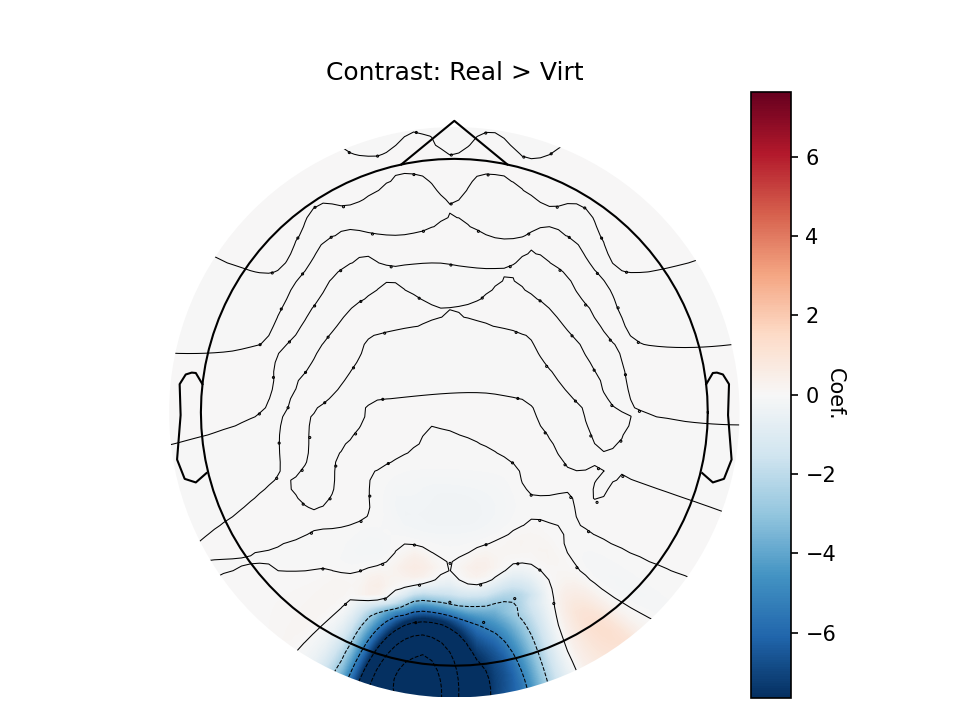
\includegraphics[width=0.7\textwidth]{C:/Users/super/OneDrive - Ontario Tech University/fNIRS_Emotions/plots/glm/contrasts/differences/Contrast_Real-Virt.png}
      \caption[GLM: Real vs. Virtual Faces]{GLM contrast between real and virtual conditions which shows the differences in activation between the two conditions.
      Red signifies that condition 1 (real faces) has more activation in that area than condition 2 (virtual faces), while blue signifies that condition 2 (virtual faces) has more activation than condition 1 (real faces).
      The color bar on the right shows the coefficient of the contrast, which indicates the strength of the difference in activation between the two conditions.}
      \label{fig:glm_real_vs_virtual}
\end{figure}

\noindent
\textbf{Neural Responses to different emotions}

Pairwise contrasts with Neutral (control) and other emotions revealed significant differences in activation across several brain regions (Figure \ref{fig:glm_emotion_analysis_neutral}). 
For instance, perceiving Anger, Fear, and Joy elicited less activity in the right occipital region than perceiving Neutral. 
Morever, processing Joy was associated with less activity in the right parietal region, while processing Sadness produced less activity in the left frontal region relative to processing Neutral. 
These results indicate distinct neural activation patterns for each emotion when contrasted against the "baseline" Neutral condition, with most prominent differences in neural activity over the occipital region. 

\begin{figure}[H]
    \centering
    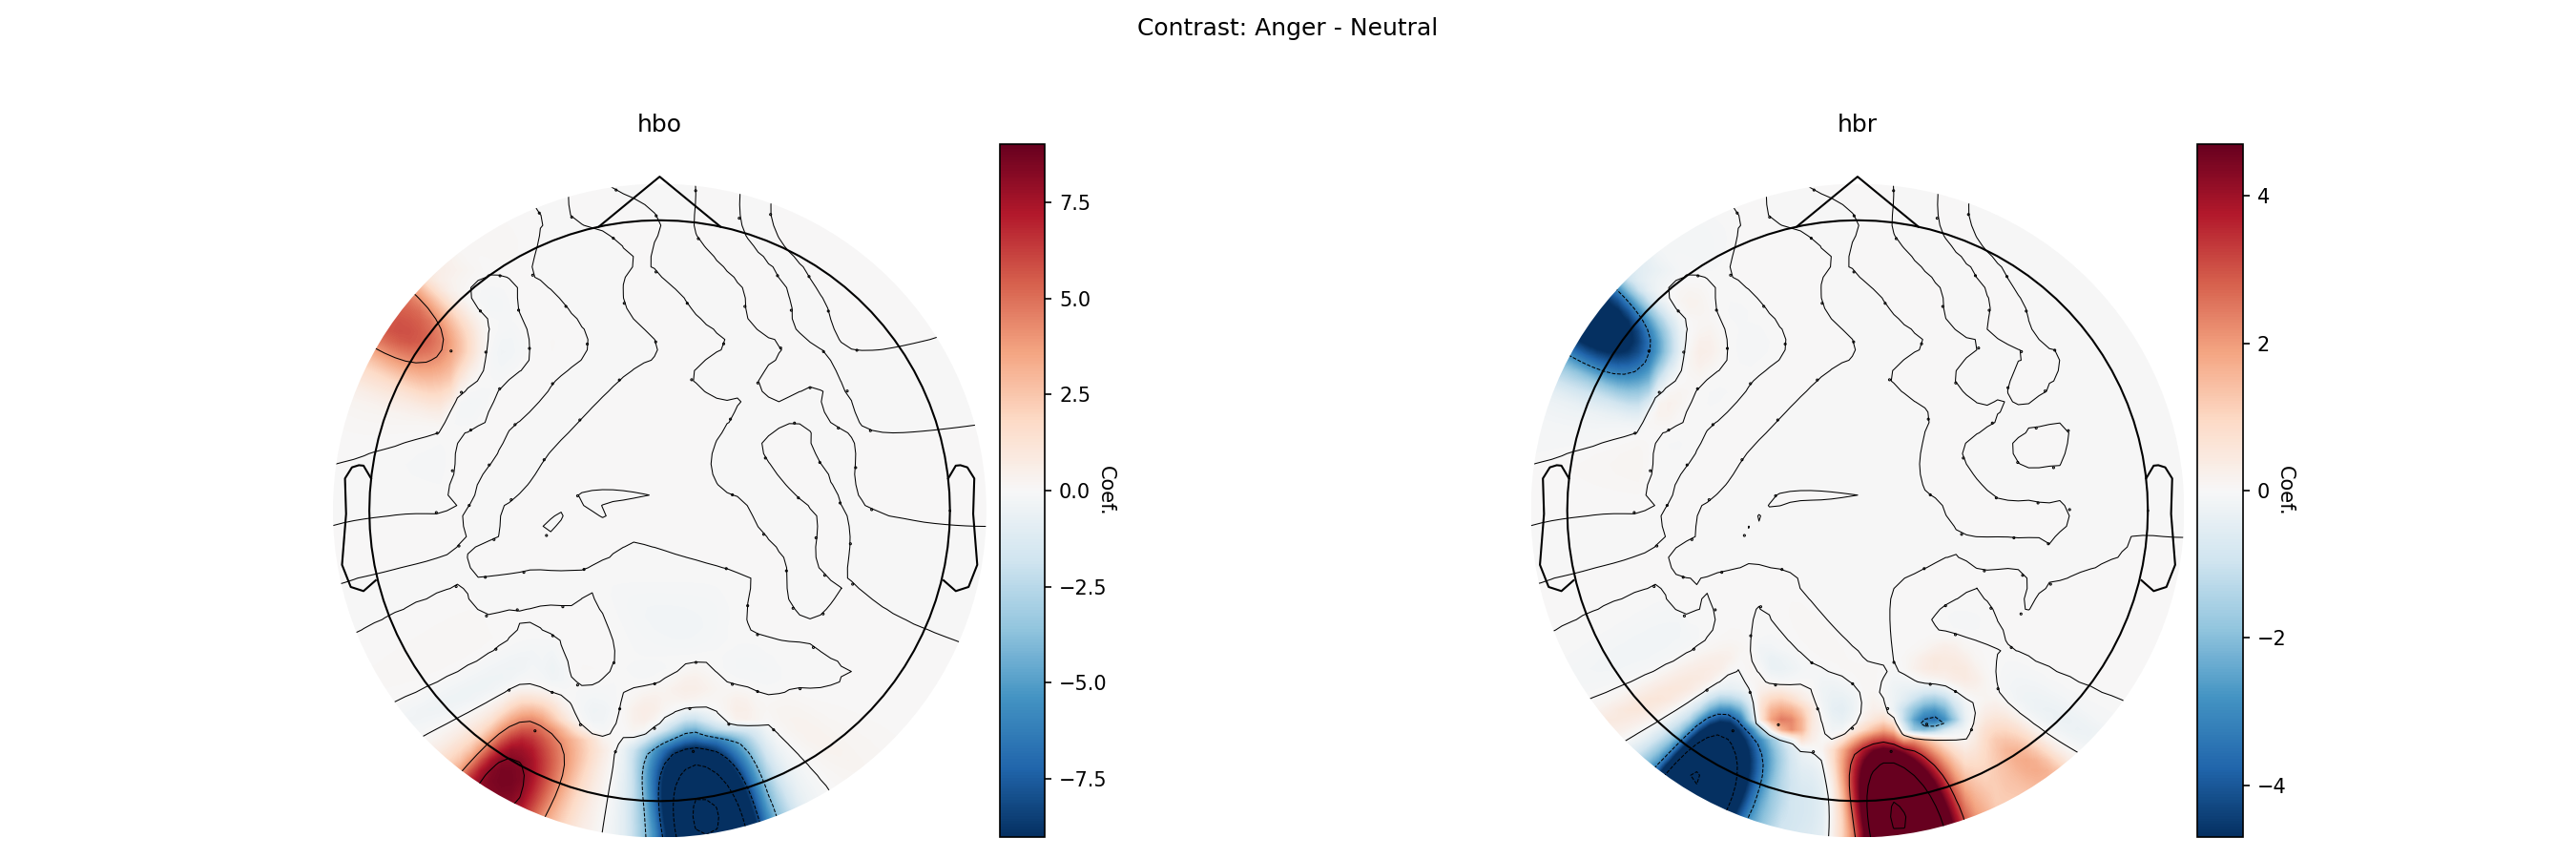
\includegraphics[width=0.49\textwidth]{C:/Users/super/OneDrive - Ontario Tech University/fNIRS_Emotions/plots/glm/contrasts/differences_neutral/Contrast_Anger-Neutral.png}
    
\includegraphics[width=0.49\textwidth]{C:/Users/super/OneDrive - Ontario Tech University/fNIRS_Emotions/plots/glm/contrasts/differences_neutral/Contrast_Fear-Neutral.png}
    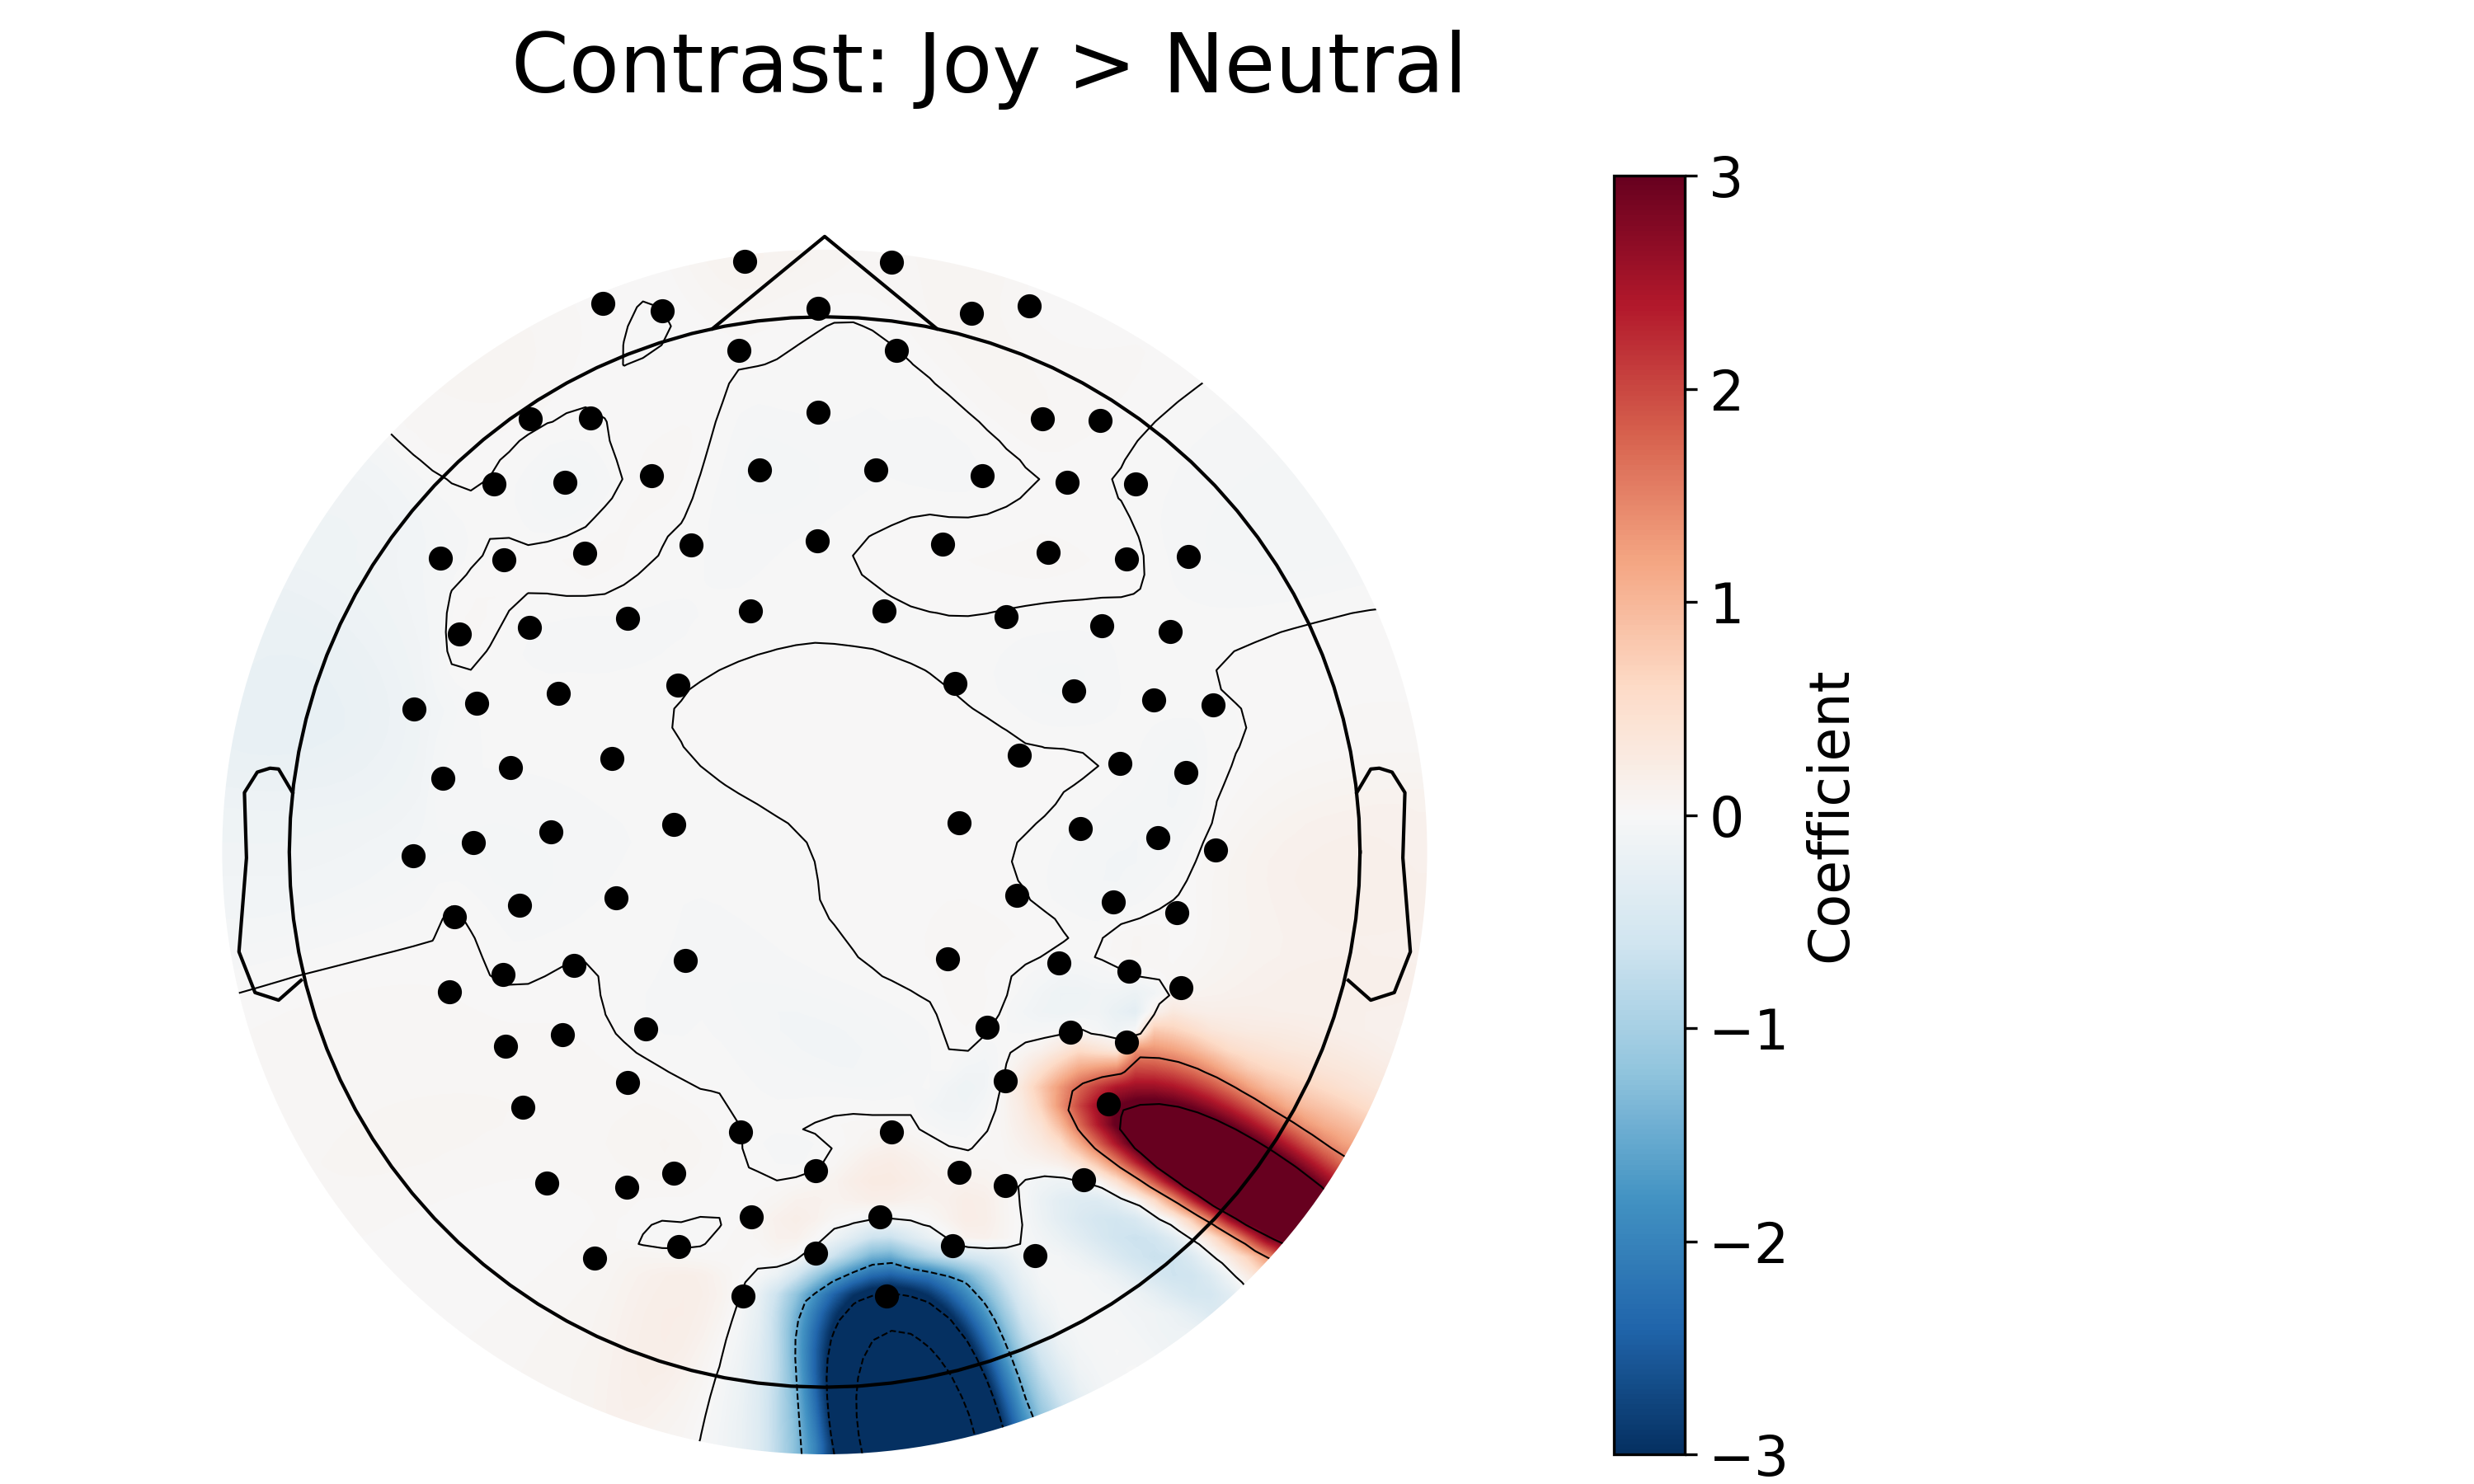
\includegraphics[width=0.49\textwidth]{C:/Users/super/OneDrive - Ontario Tech University/fNIRS_Emotions/plots/glm/contrasts/differences_neutral/Contrast_Joy-Neutral.png}
    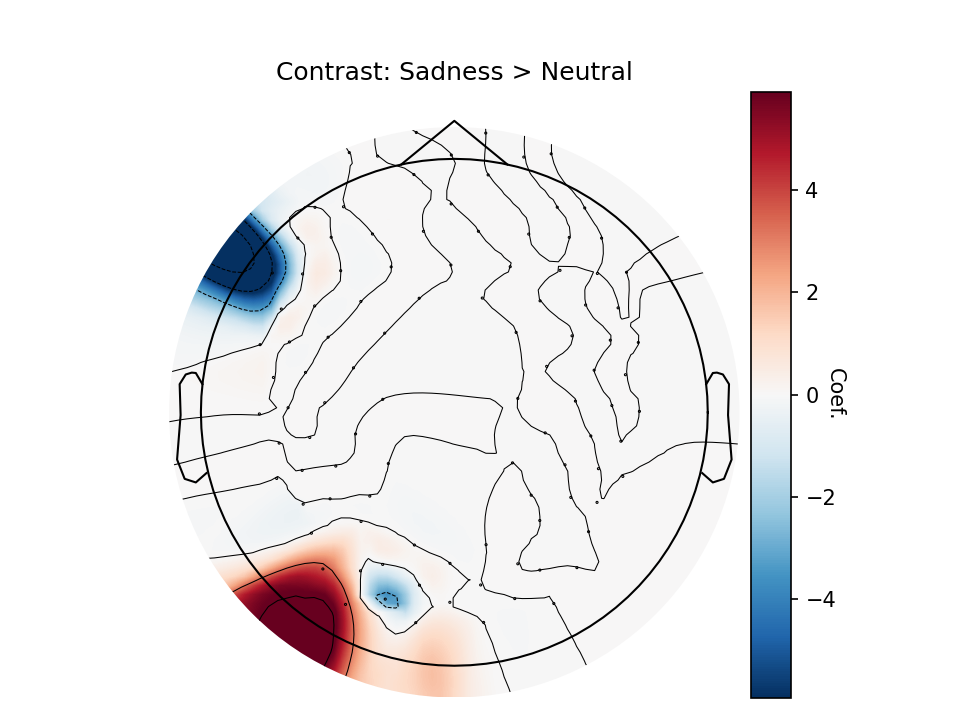
\includegraphics[width=0.49\textwidth]{C:/Users/super/OneDrive - Ontario Tech University/fNIRS_Emotions/plots/glm/contrasts/differences_neutral/Contrast_Sadness-Neutral.png}
    \caption[GLM: Emotion vs. Neutral]{GLM results for the contrast between different emotions and neutral condition.}
    \label{fig:glm_emotion_analysis_neutral}
\end{figure}

Interestingly, processing Surprise was most consistently different from processing other emotions (Figure \ref{fig:glm_emotion_analysis_surprise}). 
We found processing Surprise produced 1) more activity in the left central/temporal and right occipital regions relative to processing Disgust and Joy, 
2) more activity in the right parietal region relative to processing Fear, 3) more activity in the left frontal and right parietal regions relative to processing Sadnessl, and
4) more activity in the right parietal region and less activity in the right occipital region relative to processing Neutral.
These findings suggest that Surprise is distinct from processing Neutral but also other emotions, with differences in neural activity more widespread that include central/temporal and parietal regions. 
All combinations of emotion contrasts were performed, significant differences were only found between Neutral relative to the other emotions, and between Surprise relative to the other emotions.

\begin{figure}[H]
    \centering
      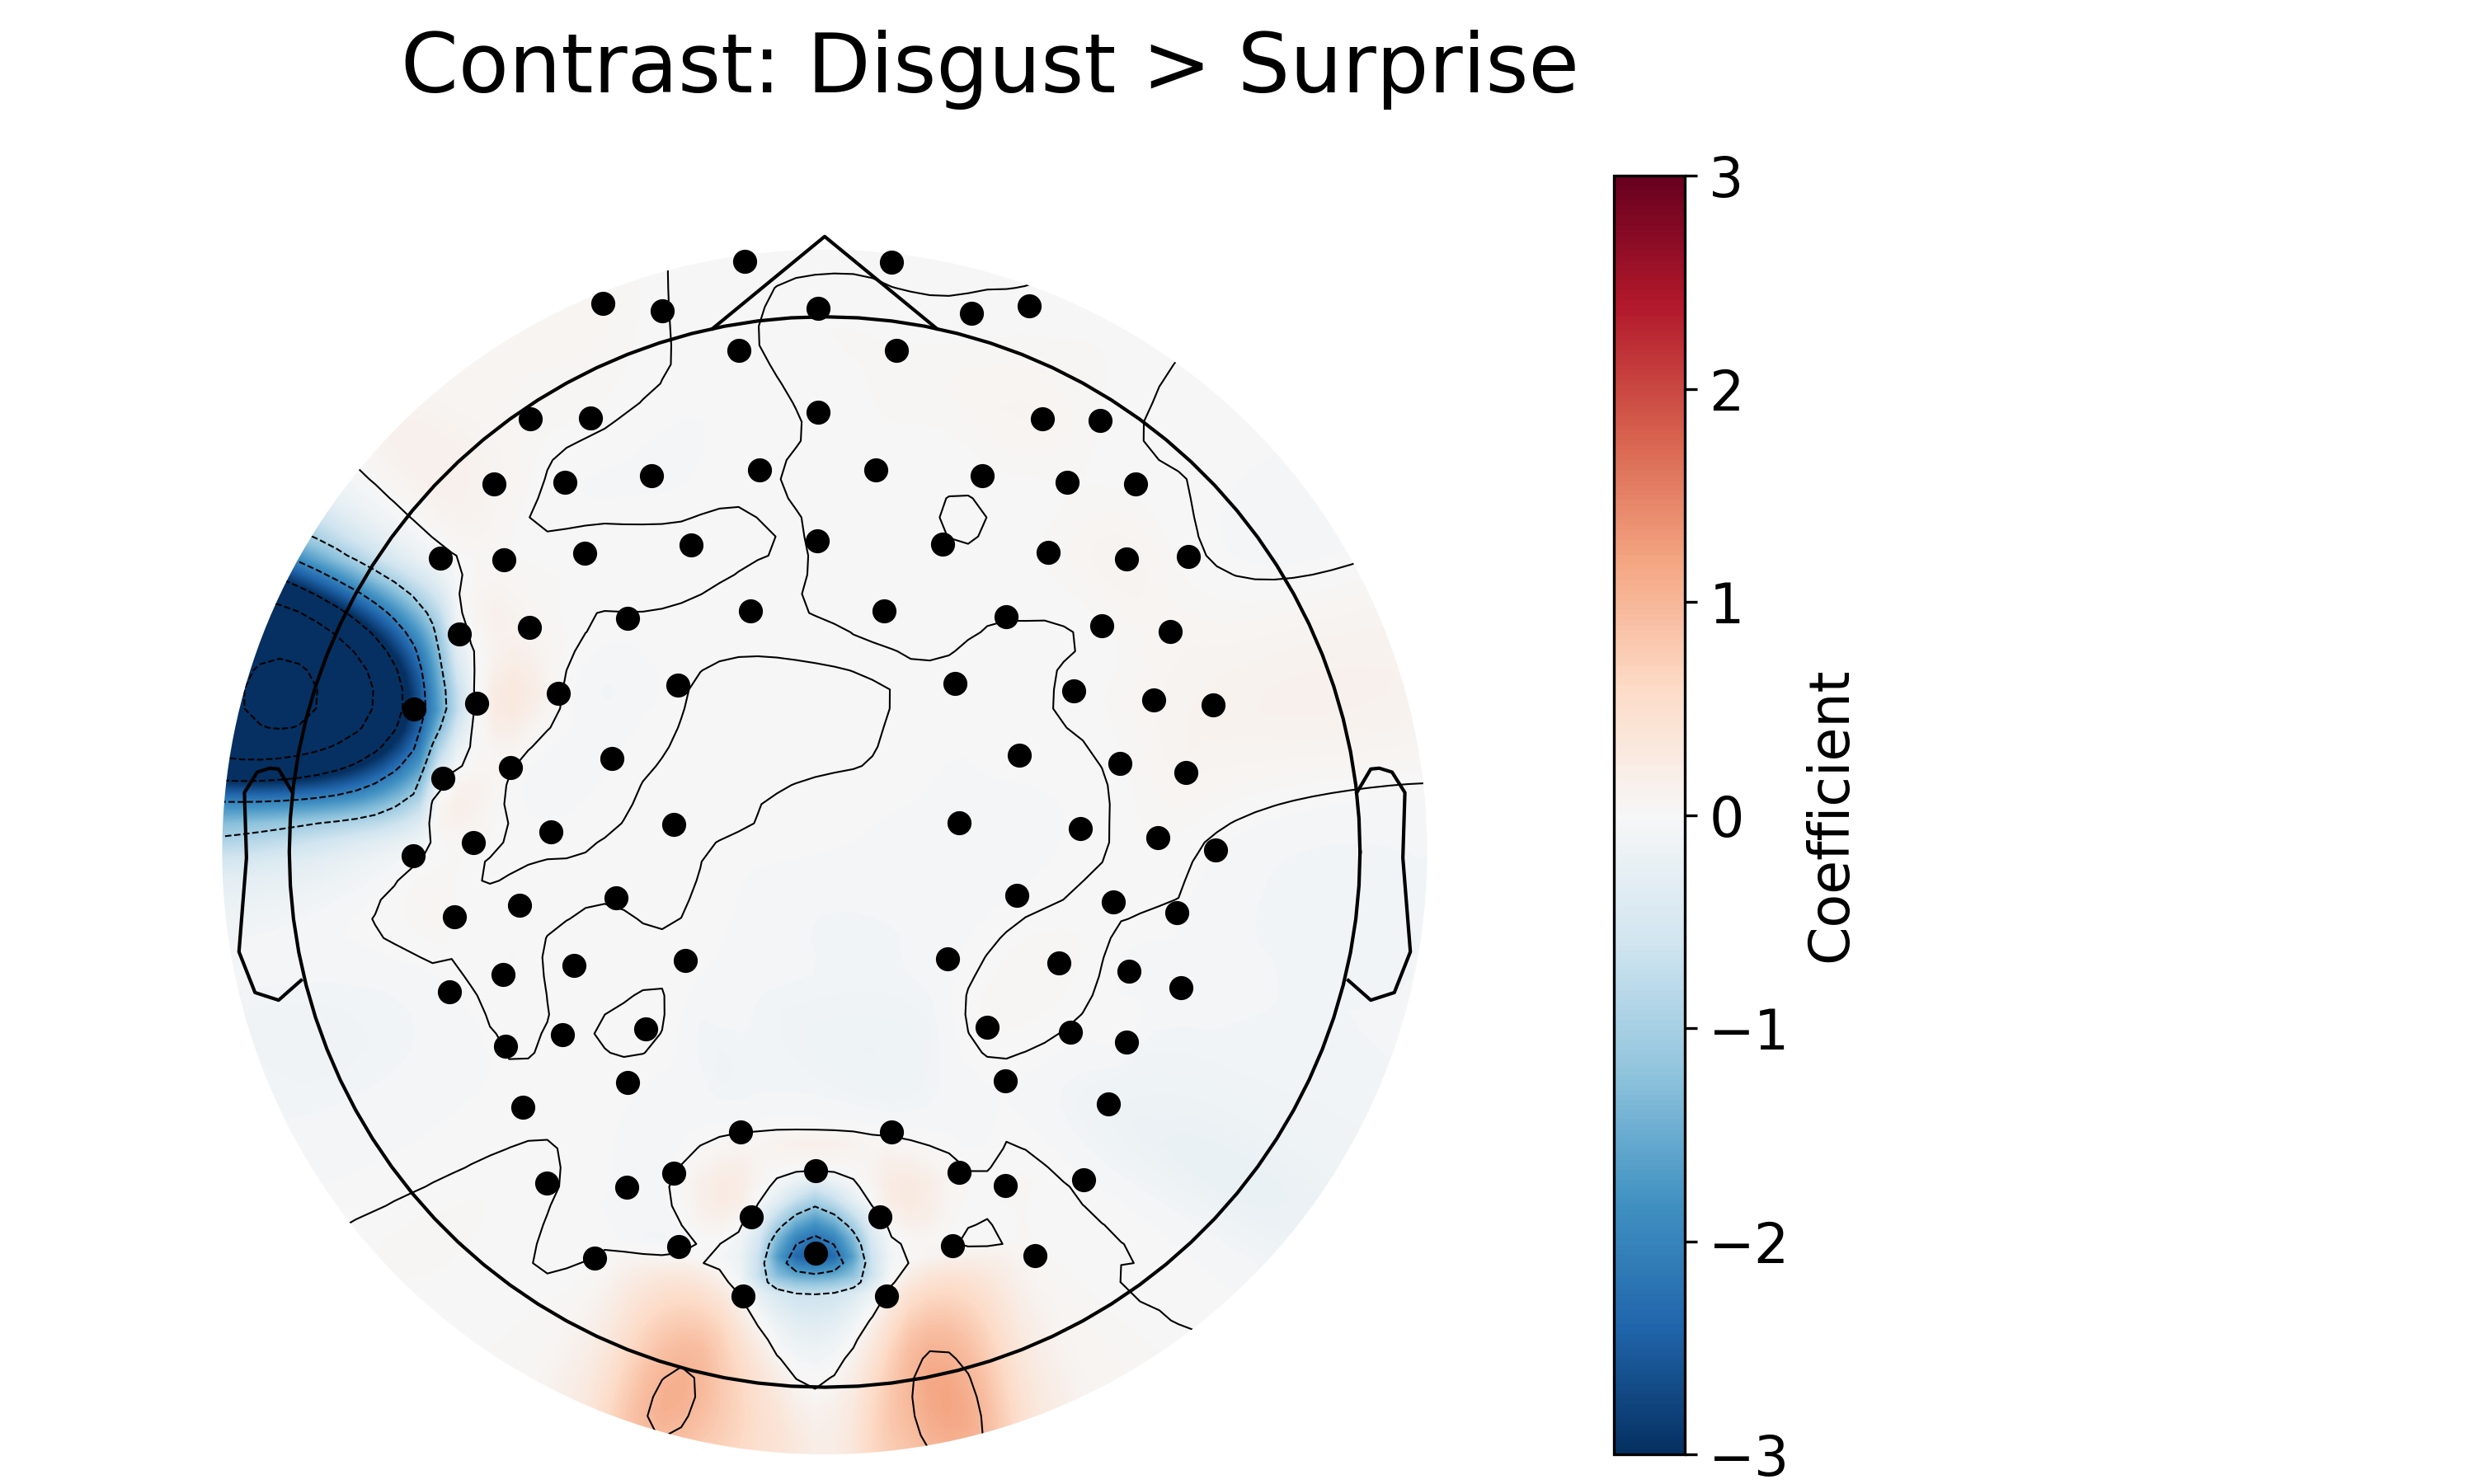
\includegraphics[width=0.49\textwidth]{C:/Users/super/OneDrive - Ontario Tech University/fNIRS_Emotions/plots/glm/contrasts/differences/Contrast_Disgust-Surprise.png}
      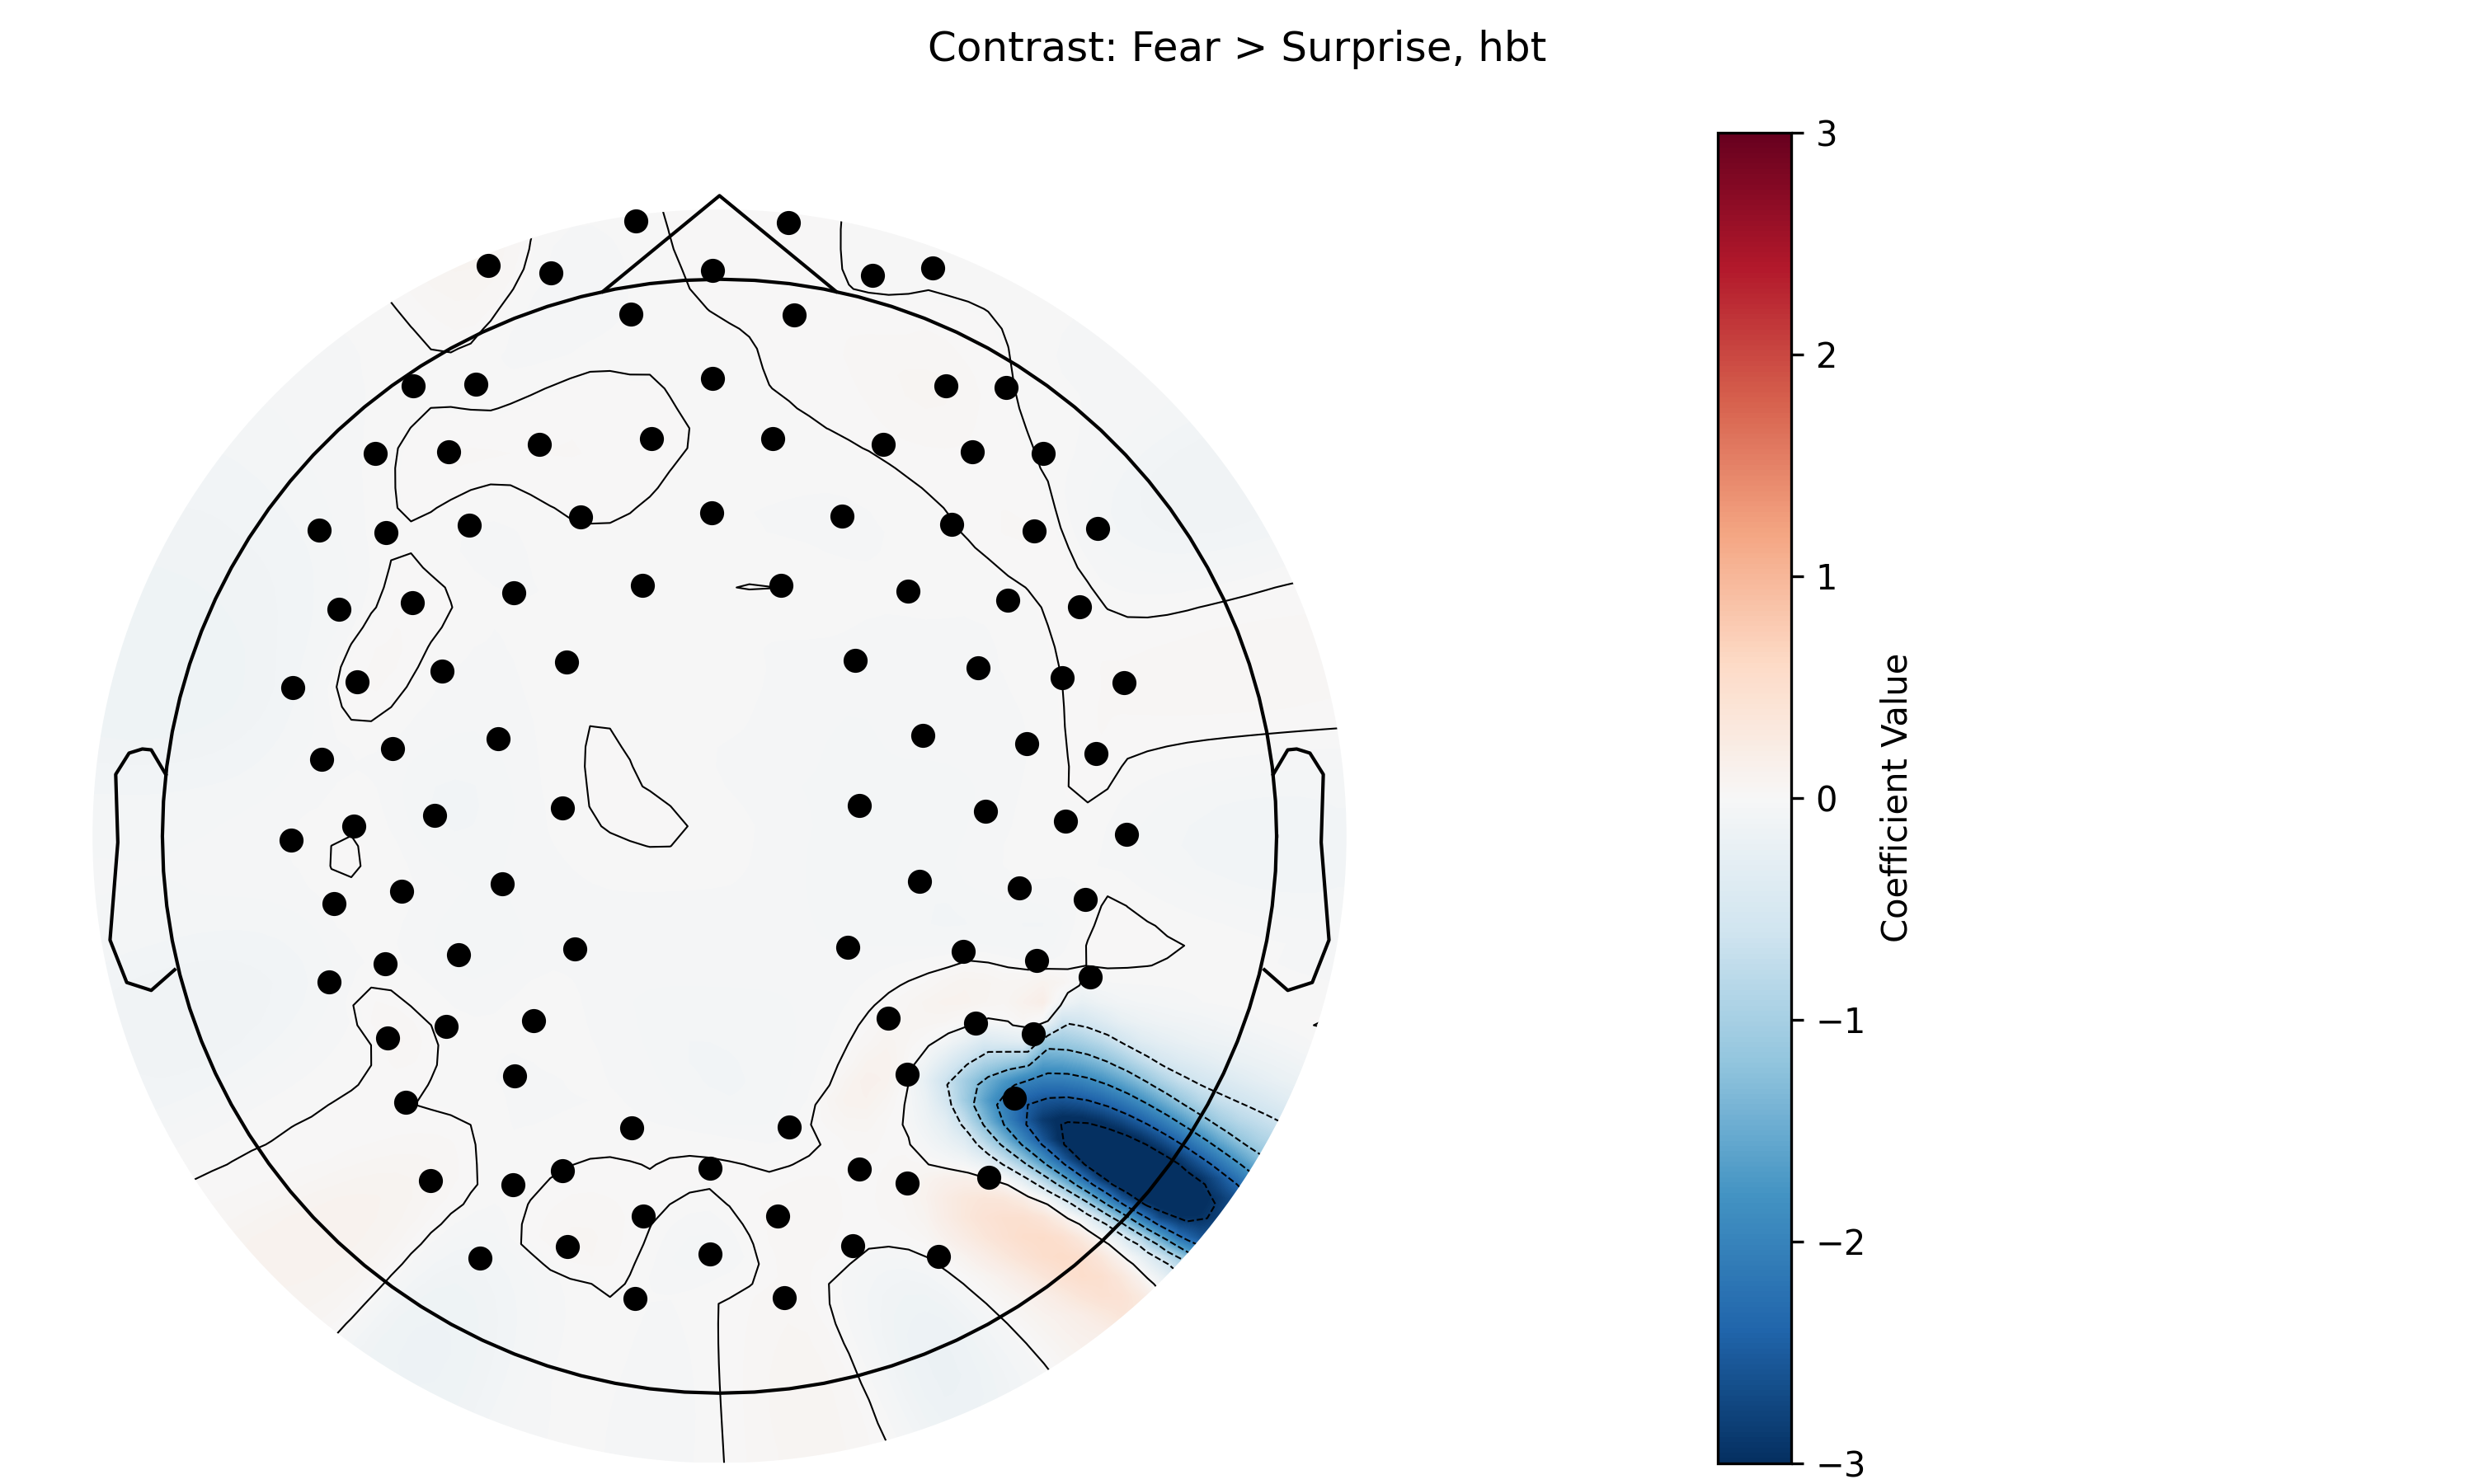
\includegraphics[width=0.49\textwidth]{C:/Users/super/OneDrive - Ontario Tech University/fNIRS_Emotions/plots/glm/contrasts/differences/Contrast_Fear-Surprise.png}
      
\includegraphics[width=0.49\textwidth]{C:/Users/super/OneDrive - Ontario Tech University/fNIRS_Emotions/plots/glm/contrasts/differences/Contrast_Joy-Surprise.png}
      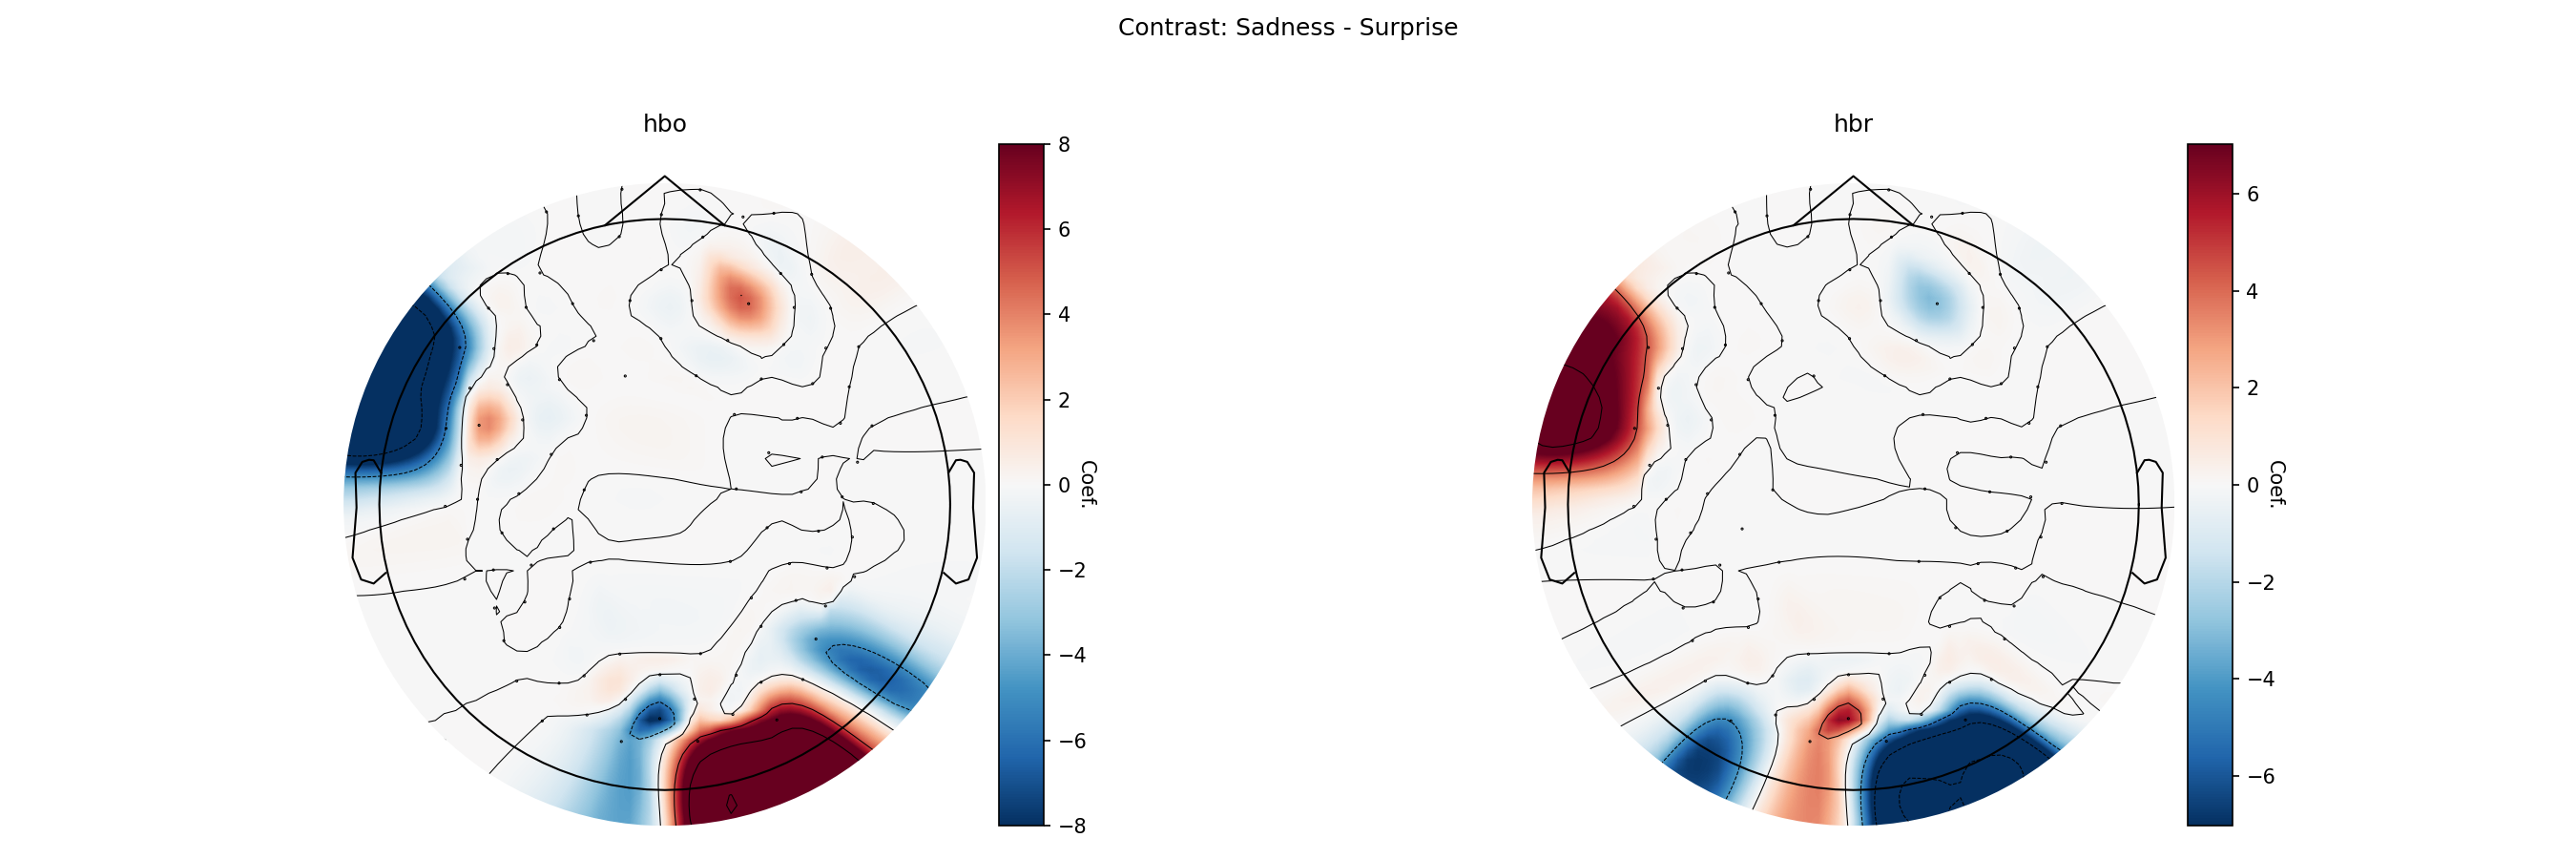
\includegraphics[width=0.49\textwidth]{C:/Users/super/OneDrive - Ontario Tech University/fNIRS_Emotions/plots/glm/contrasts/differences/Contrast_Sadness-Surprise.png}
      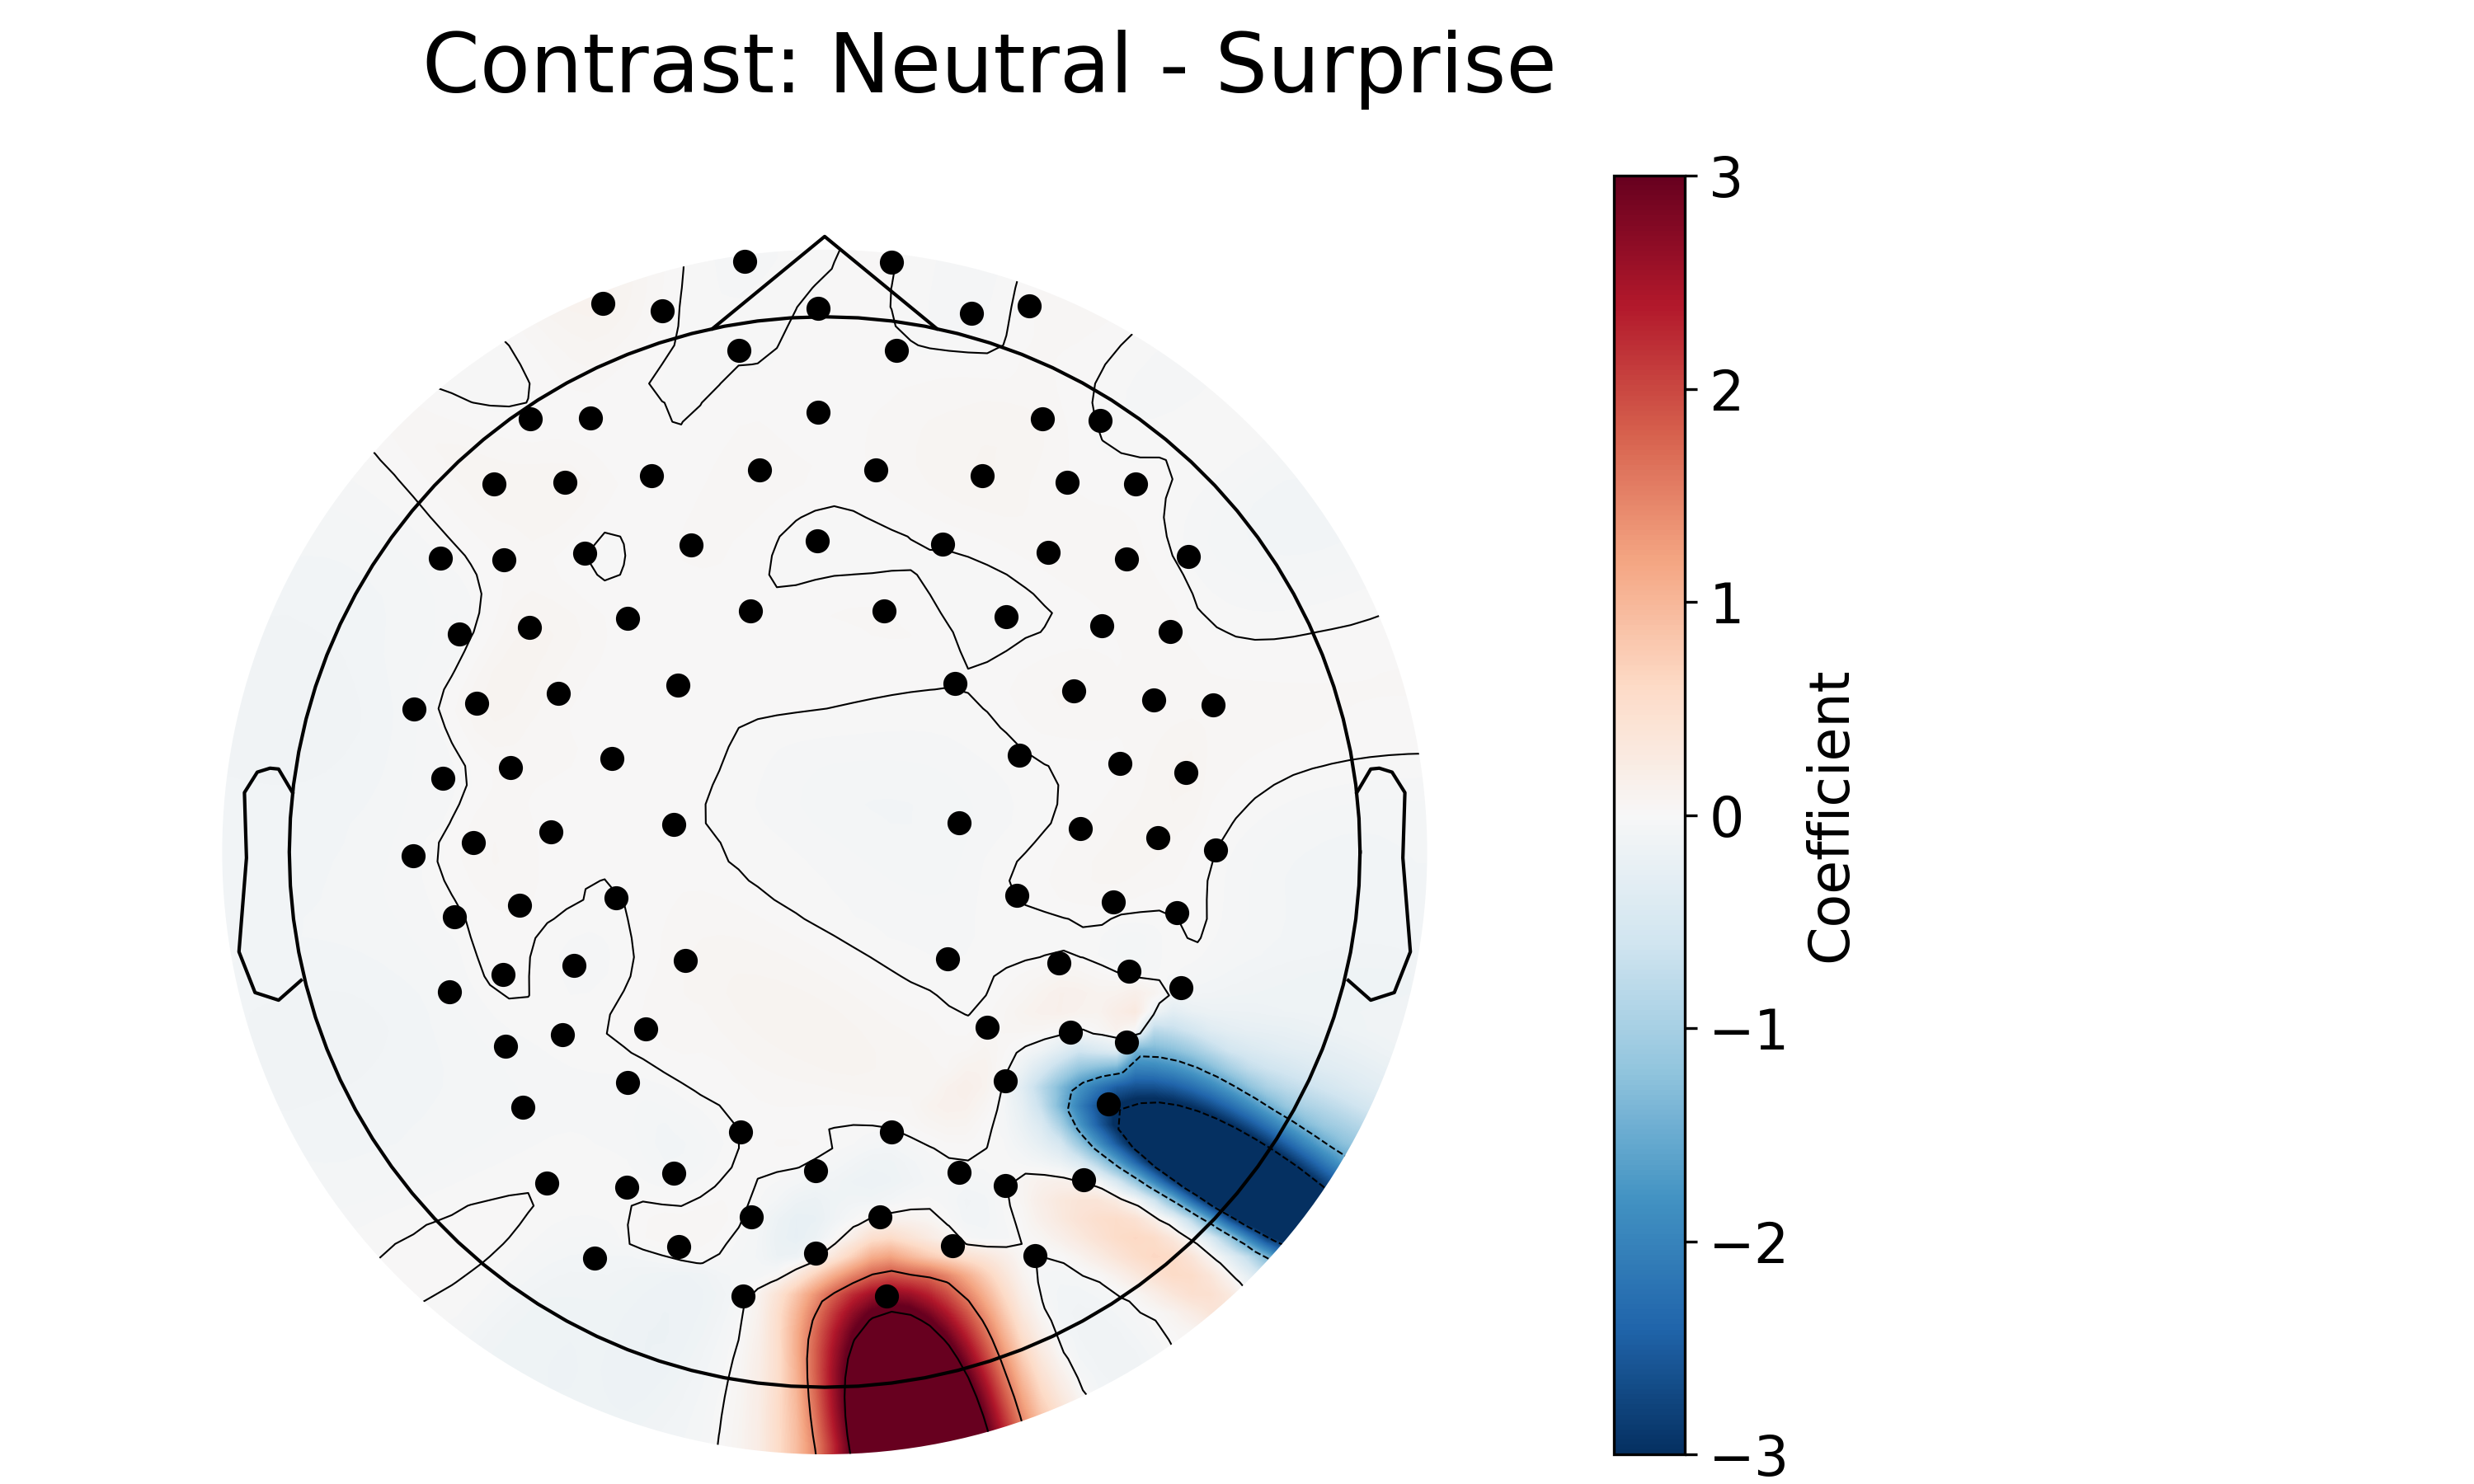
\includegraphics[width=0.55\textwidth]{C:/Users/super/OneDrive - Ontario Tech University/fNIRS_Emotions/plots/glm/contrasts/differences_neutral/Contrast_Neutral-Surprise.png}
      \caption[GLM: Emotion vs. Surprise]{GLM results for the contrast between different emotions and surprise condition.}
      \label{fig:glm_emotion_analysis_surprise}
\end{figure}

\noindent
\textbf{Differential neural responses to emotions and face type}

The interaction of Real $>$ Virtual within each emotion, as shown in Figure \ref{fig:glm_real_vs_virtual_emotion_analysis} revealed significant differences in occipital regions exclusively.
Specifically, processing Disgust on real faces elicited greater activity in the right occipital region compared to processing Disgust on virtual faces, whereas the left occipital region showed the opposite pattern.
Moreover, processing Joy and Neutral emotions on real faces also elicited greater activity in the occipital regions compared to processing the same emotions on virtual faces.
We found processing Sadness on virtual faces produced more activity in the left occipital region for virtual faces compared to processing Sadness on real faces. 
These findings suggest that the neural response to emotional expressions is modulated by the realism of the face stimuli. 
The full table of the GLM contrasts for all main effects and interactions can be found in Appendix \ref{tab:appendix_glm_results}.

\begin{figure}[H]
  \centering
  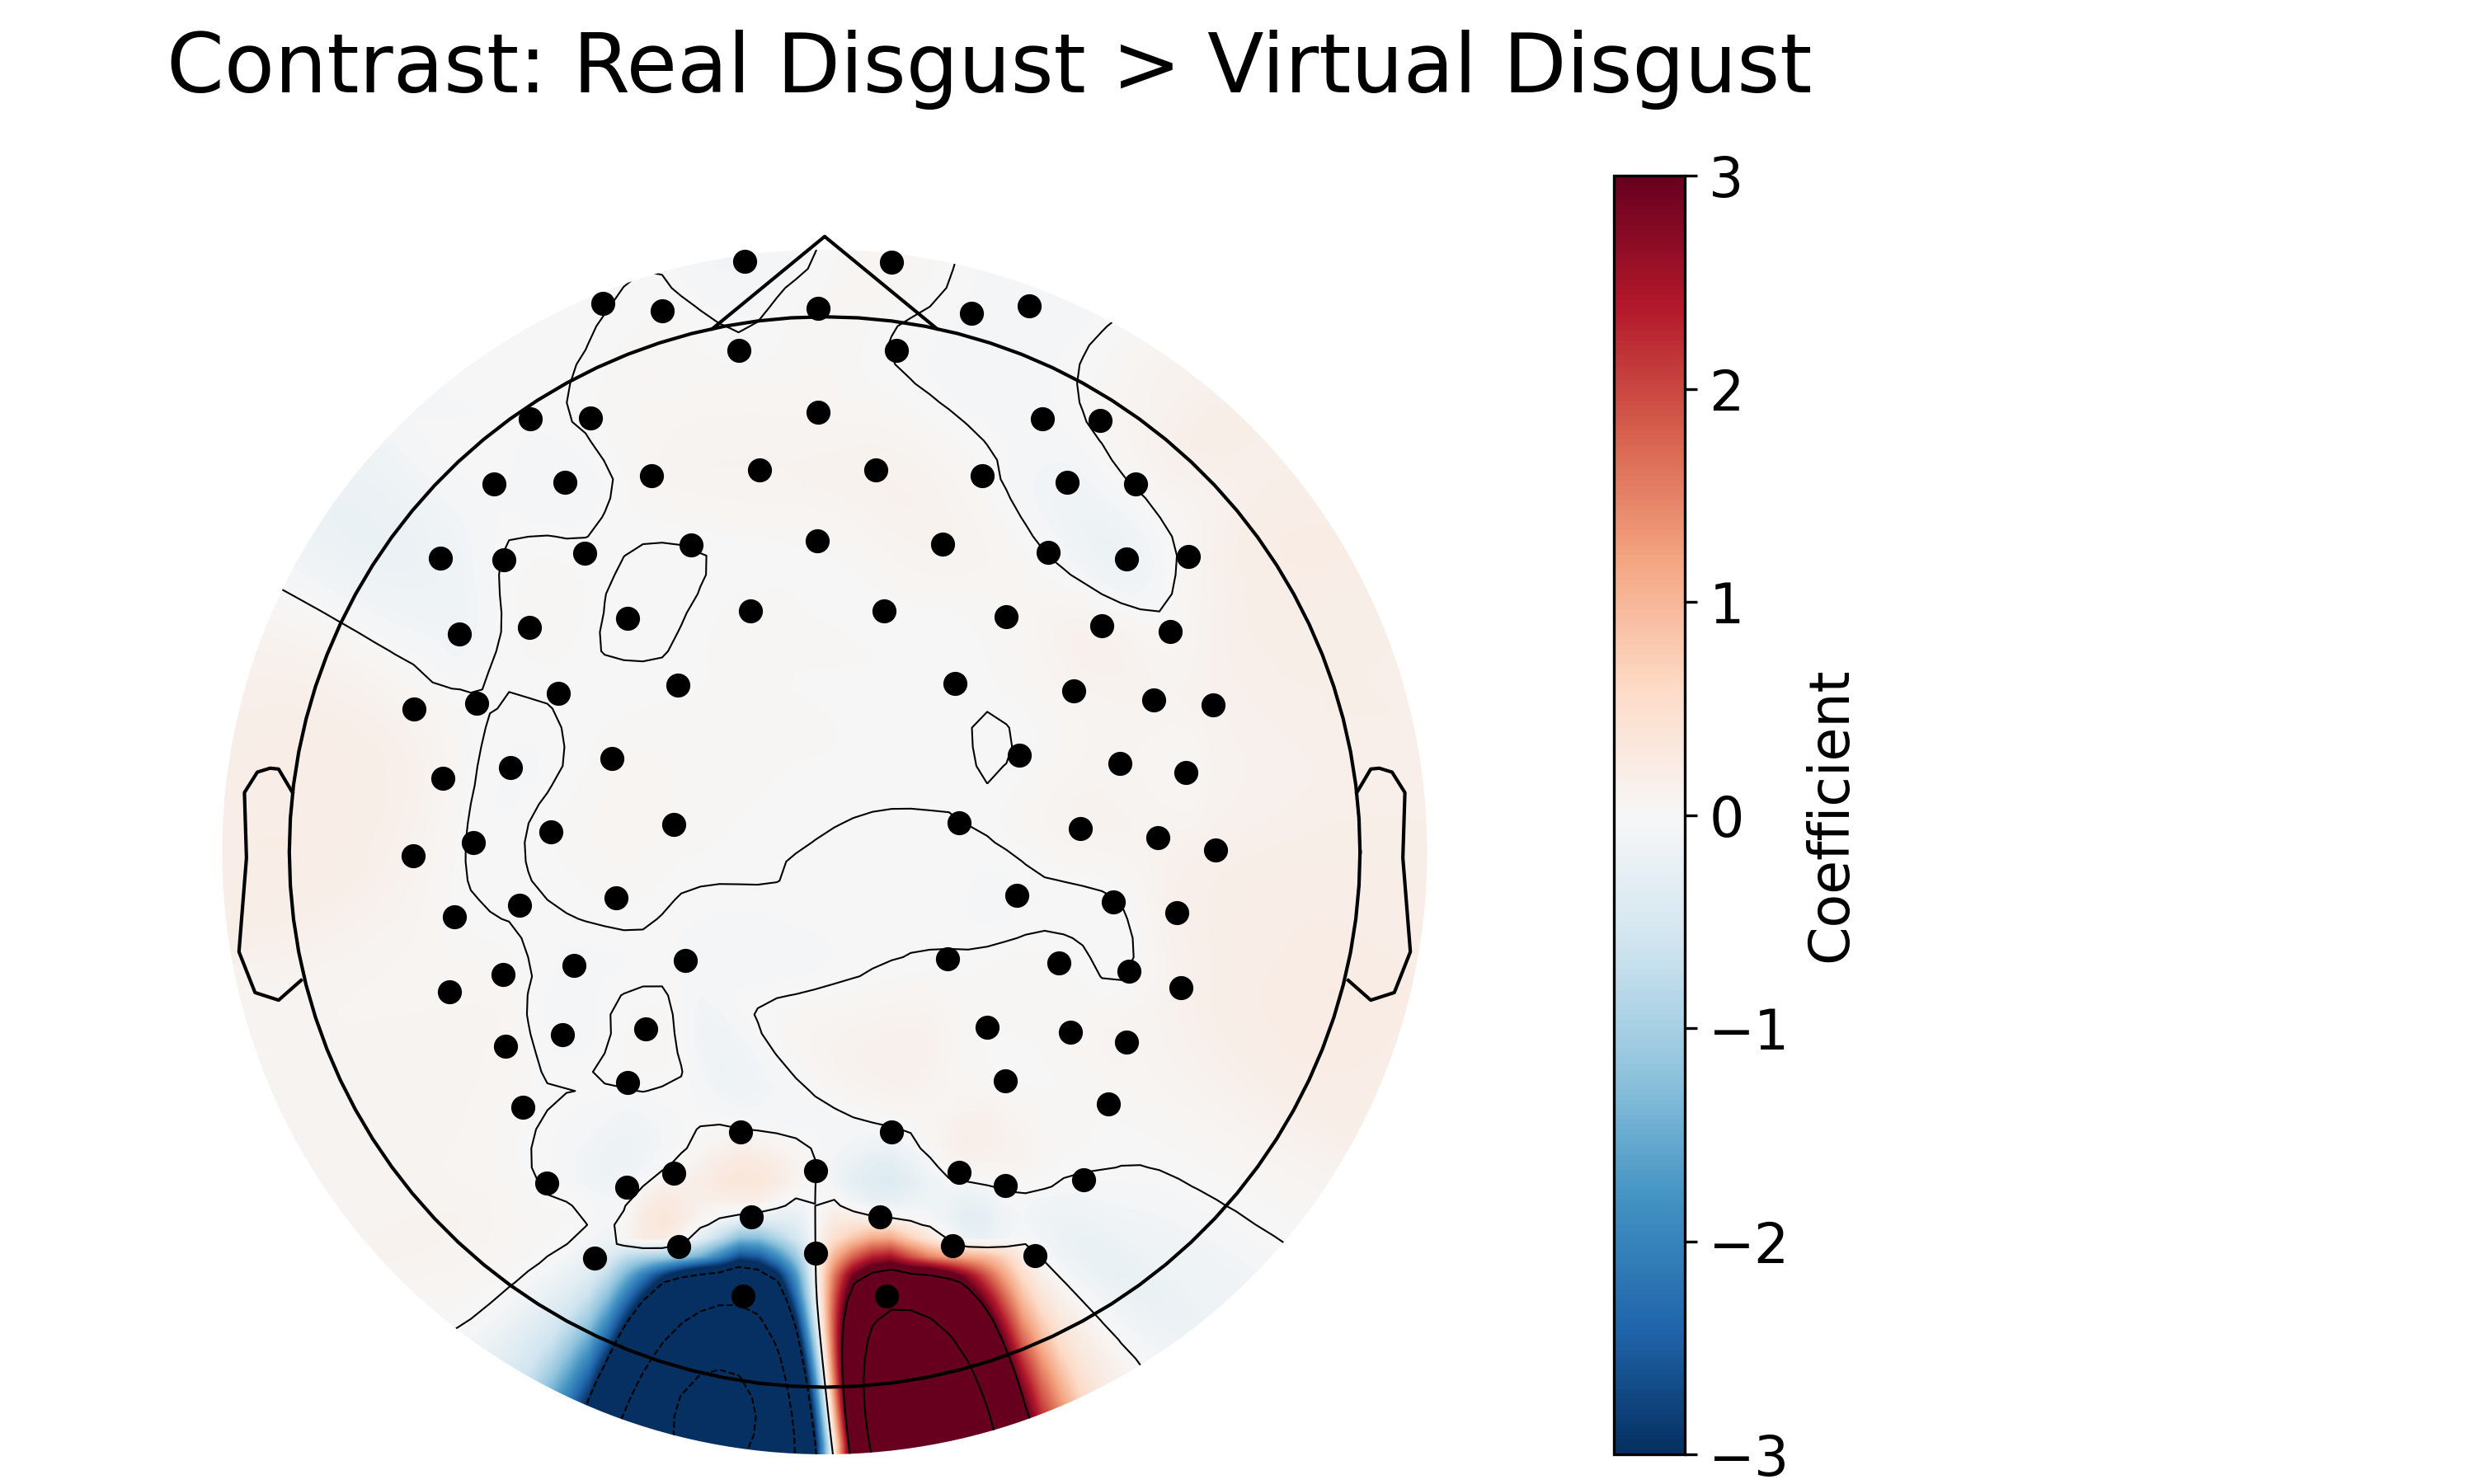
\includegraphics[width=0.49\textwidth]{C:/Users/super/OneDrive - Ontario Tech University/fNIRS_Emotions/plots/glm/contrasts/differences/Contrast_Real_Disgust-Virt_Disgust.png}
  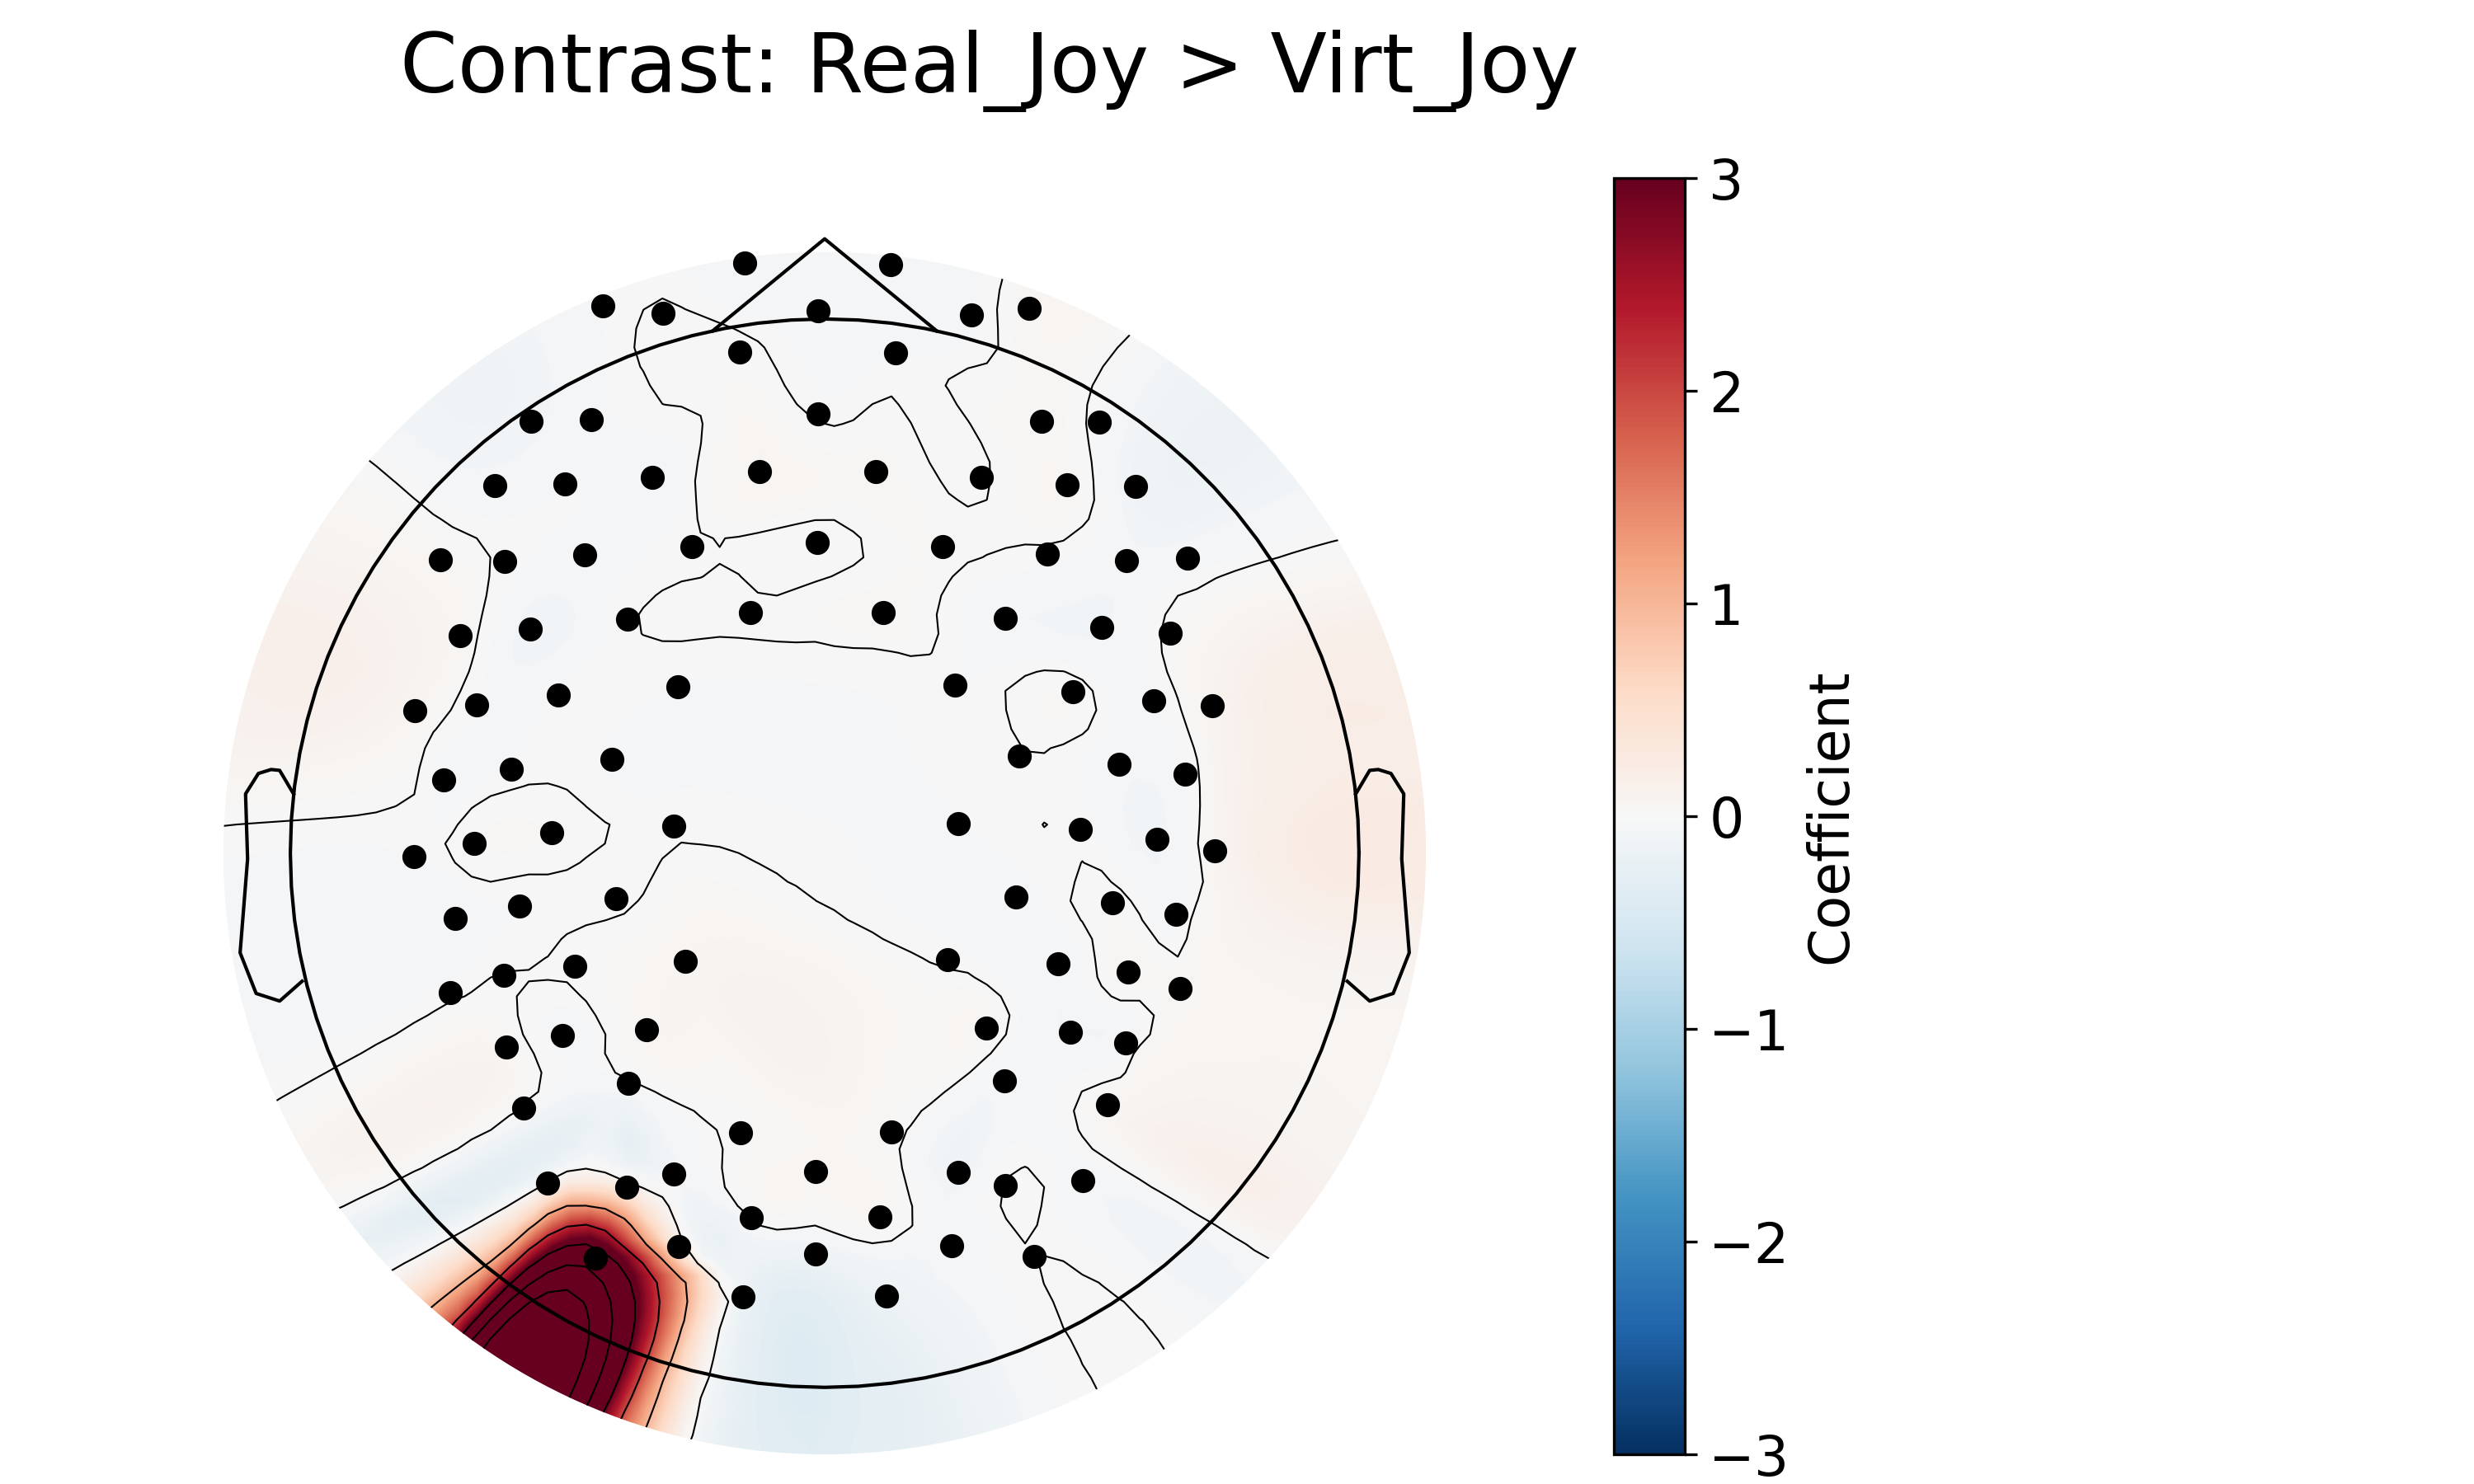
\includegraphics[width=0.49\textwidth]{C:/Users/super/OneDrive - Ontario Tech University/fNIRS_Emotions/plots/glm/contrasts/differences/Contrast_Real_Joy-Virt_Joy.png}
  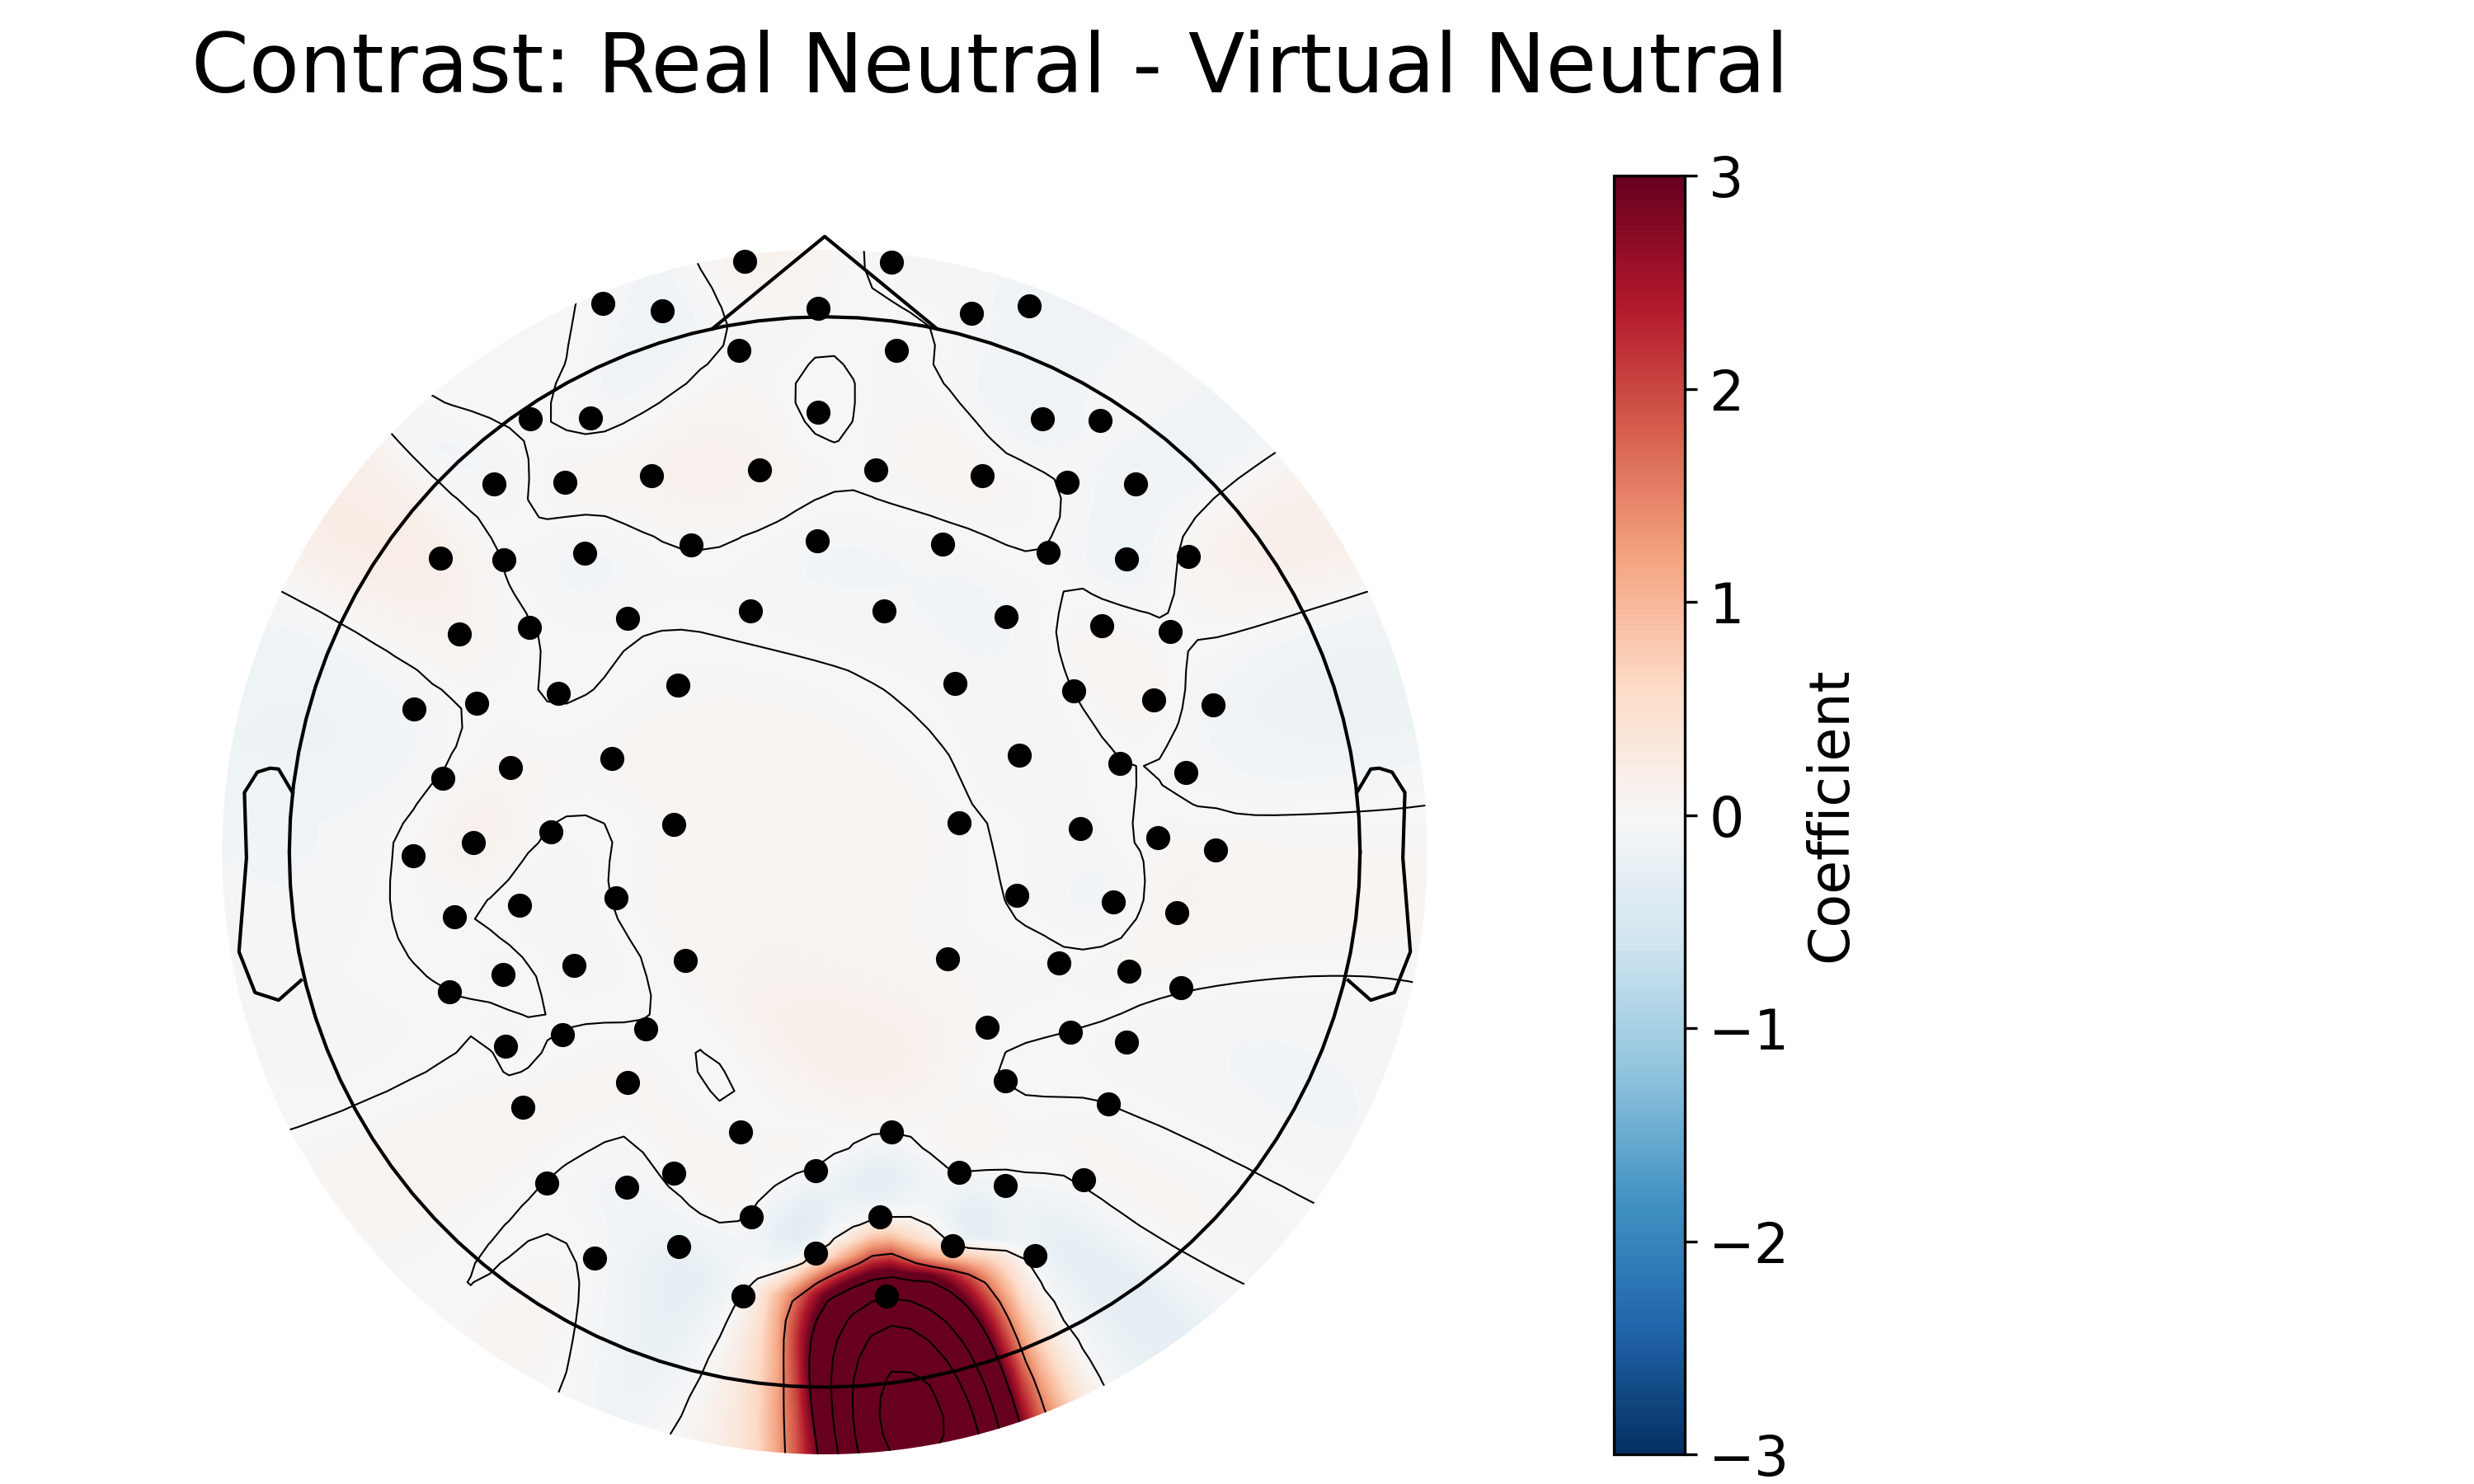
\includegraphics[width=0.49\textwidth]{C:/Users/super/OneDrive - Ontario Tech University/fNIRS_Emotions/plots/glm/contrasts/differences/Contrast_Real_Neutral-Virt_Neutral.png}
  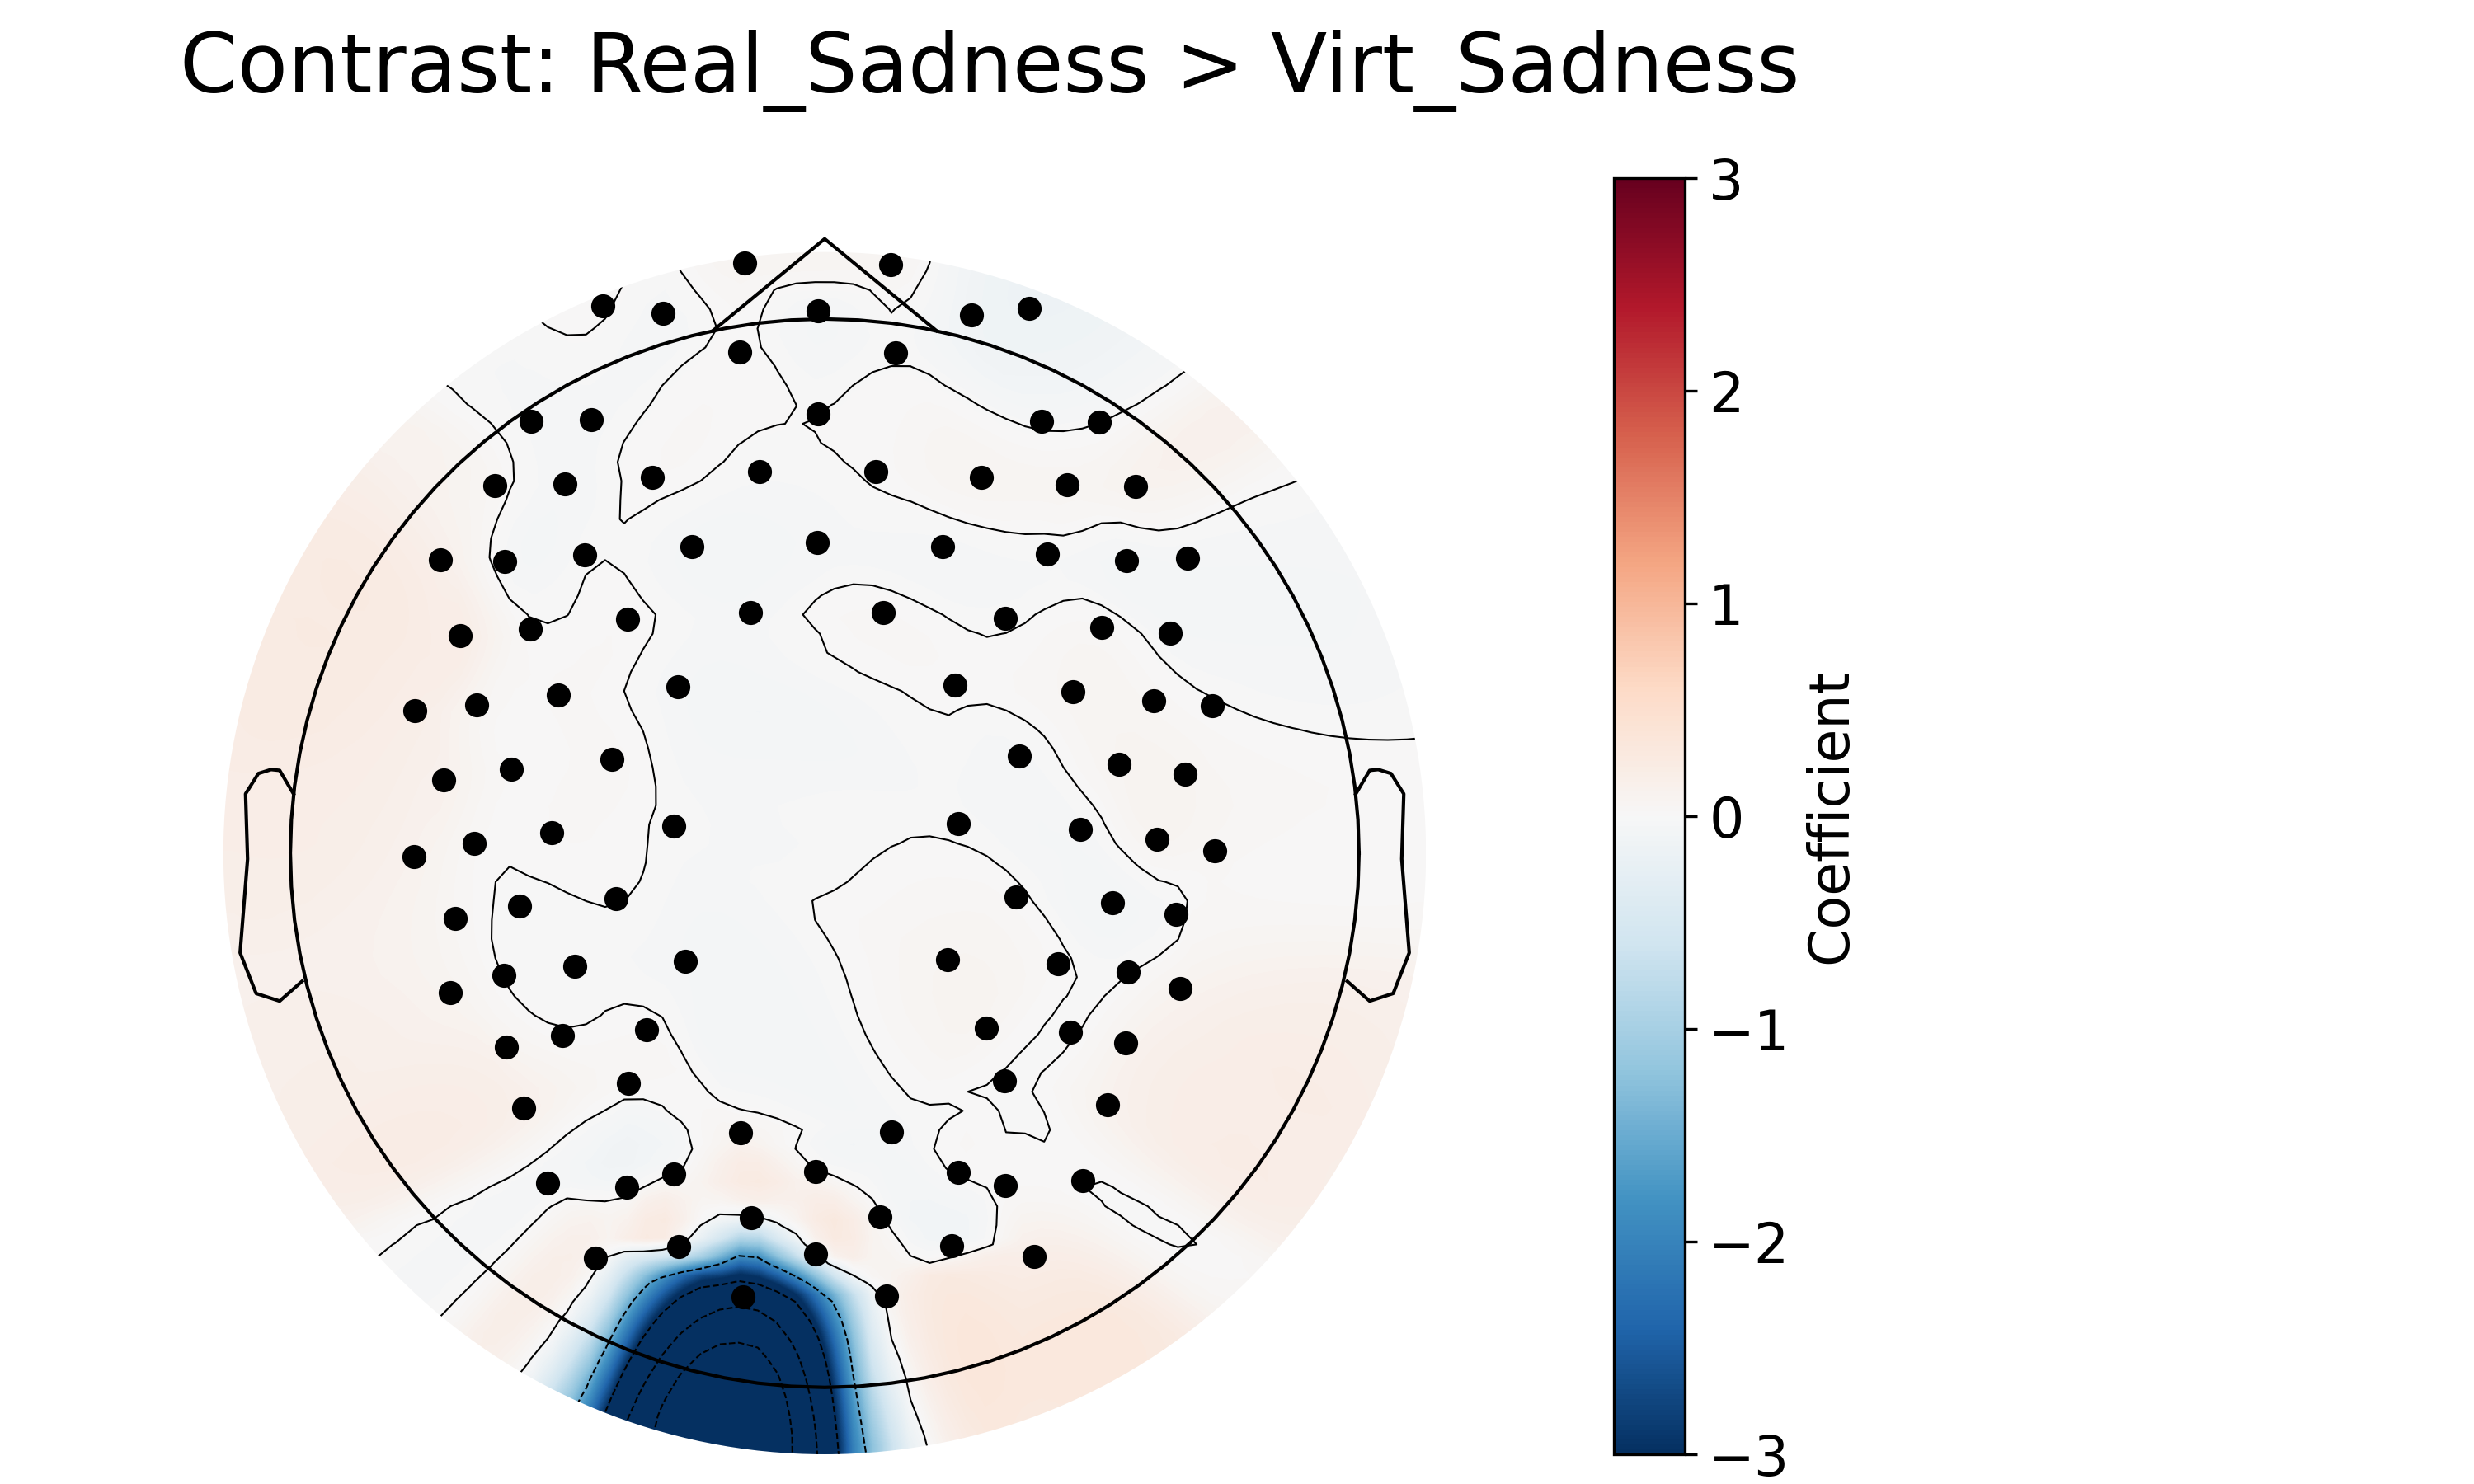
\includegraphics[width=0.49\textwidth]{C:/Users/super/OneDrive - Ontario Tech University/fNIRS_Emotions/plots/glm/contrasts/differences/Contrast_Real_Sadness-Virt_Sadness.png}
  \caption[GLM: Face Type \texorpdfstring{$\times$}{x} Emotion Contrasts]{GLM results for the contrast between real and virtual conditions within each emotion.}
  \label{fig:glm_real_vs_virtual_emotion_analysis}
\end{figure}

\section{Functional Connectivity Results}
\noindent
\textbf{Functional connectivity profiles of face type}

The contrast comparing functional connectivity profiles in response to real versus virtual faces (as shown in Figure \ref{fig:fc_real_vs_virtual}) revealed significant differences in connectivity across the brain. 
Processing real faces was associated with stronger connectivity predominantly between the left to right parietal, left frontal to left parietal, left central/temporal to left parietal, left central/temporal to right parietal, and the right central/temporal to left parietal regions, whereas processing virtual faces was associated with stronger connectivity only between the left central/temporal to right frontal region. 

\begin{figure}[H]
  \centering
  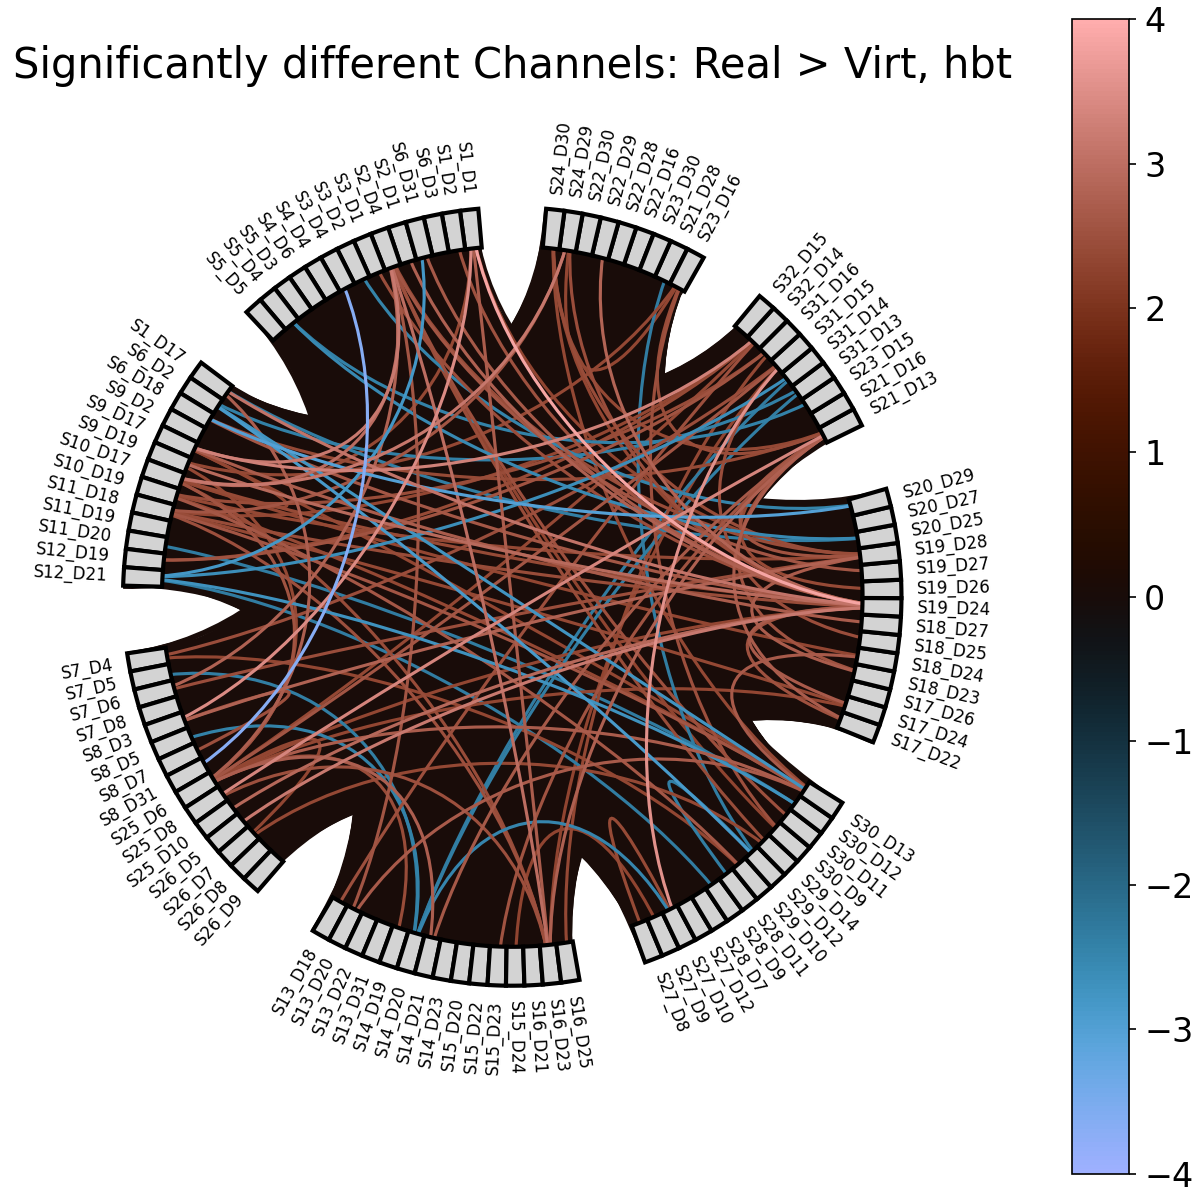
\includegraphics[width=0.7\textwidth]{C:/Users/super/OneDrive - Ontario Tech University/fNIRS_Emotions/plots/spectral_connectivity_time/chord_plots/group_level_t_tests_roi/face_type_Real_Virt.png}
  \caption[FC: Real vs. Virtual]{Functional connectivity results for the contrast between real and virtual conditions.
  The thickness of the lines represents the difference in the count of significantly different channel pairs between the two conditions. 
  A red line signifies that real faces had more significant channels between those two ROI's where the $t$-value was positive, while a blue line signifies that virtual faces had more significant channels between those two ROI's where the $t$-value was negative.
  For clarity, only the top 15th percentile of connections (those with the most significant different channel pairs) are displayed for all functional connectivity contrasts.}
  \label{fig:fc_real_vs_virtual}
\end{figure}

\noindent
\textbf{Functional connectivity in response to emotion}

We also found significant differences in functional connectivity in response to different emotions across all ROI's. 
A sample of the functional connectivity results which include only contrasts between Fear and the other emotions are plotted in Figure \ref{fig:fc_emotion_analysis}.
We found the largest connectivity differences processing faces expressing Fear relative to Neutral faces, with significantly stronger connectivity between left central/temporal and right and left frontal, and right and left parietal. 
In general, we found processing faces expressing Fear produced significantly strong connectivity across the brain relative to faces expressing all other emotions, however this difference was weakest relative to processing angry faces. 
Interestingly most of the stronger connections emerge from the left central/temporal region, pointing to this region as a key area for processing Fear. 
The complete set of functional connectivity contrasts for all emotions can be found in Appendix \ref{tab:appendix_fc_emotion_analysis}. 

\begin{figure}[H]
  \centering
  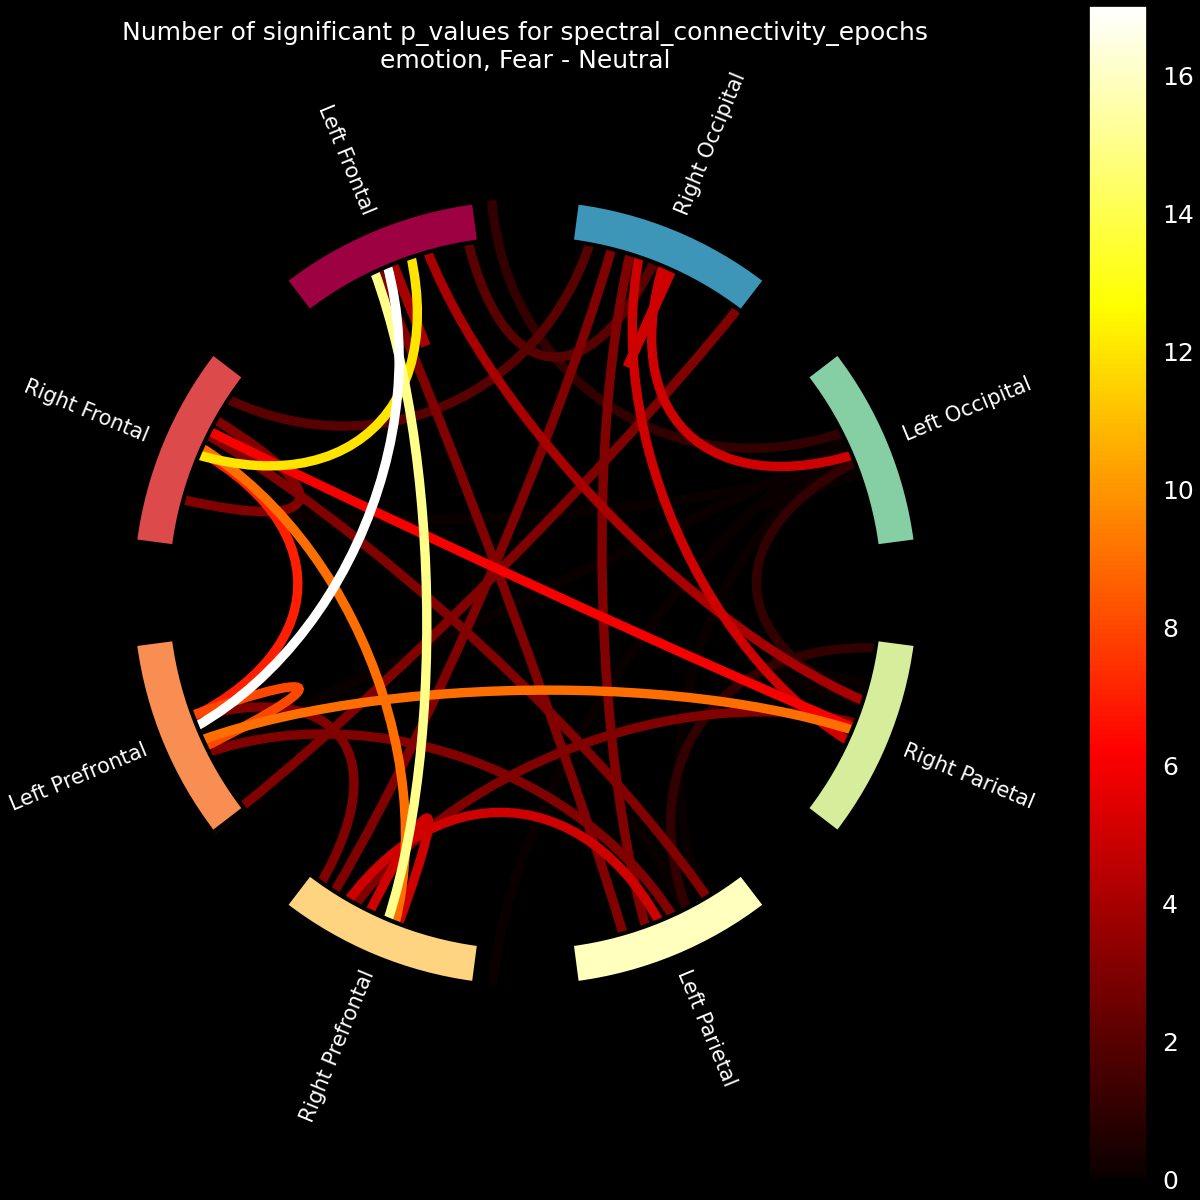
\includegraphics[width=0.32\textwidth]{C:/Users/super/OneDrive - Ontario Tech University/fNIRS_Emotions/plots/spectral_connectivity_time/chord_plots/group_level_t_tests_roi/emotion_Fear_Neutral.png}
  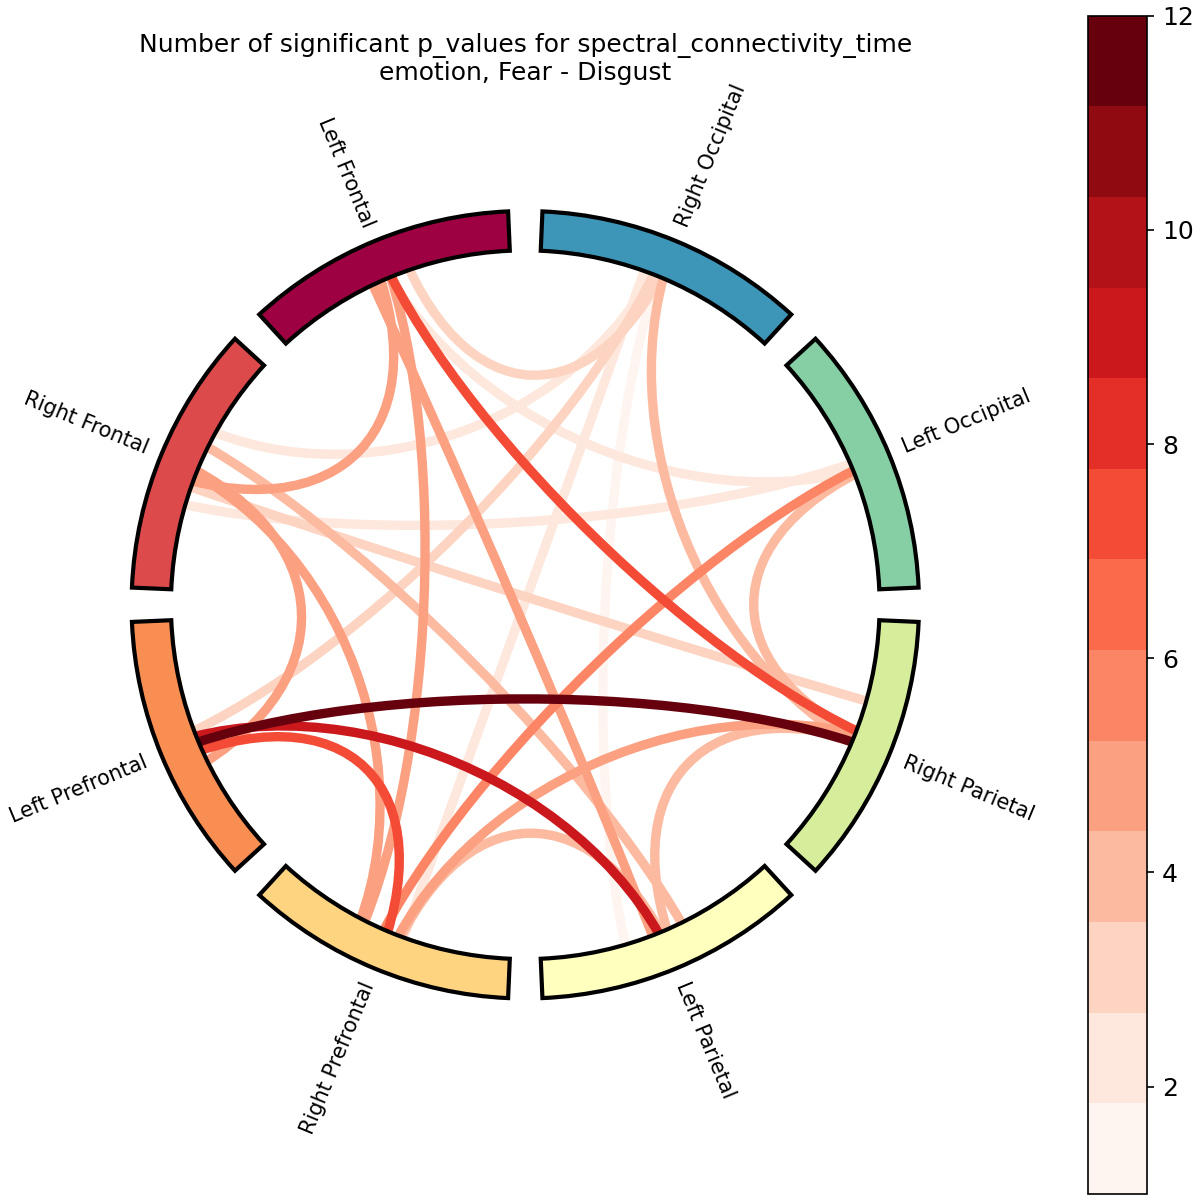
\includegraphics[width=0.32\textwidth]{C:/Users/super/OneDrive - Ontario Tech University/fNIRS_Emotions/plots/spectral_connectivity_time/chord_plots/group_level_t_tests_roi/emotion_Fear_Disgust.png}
  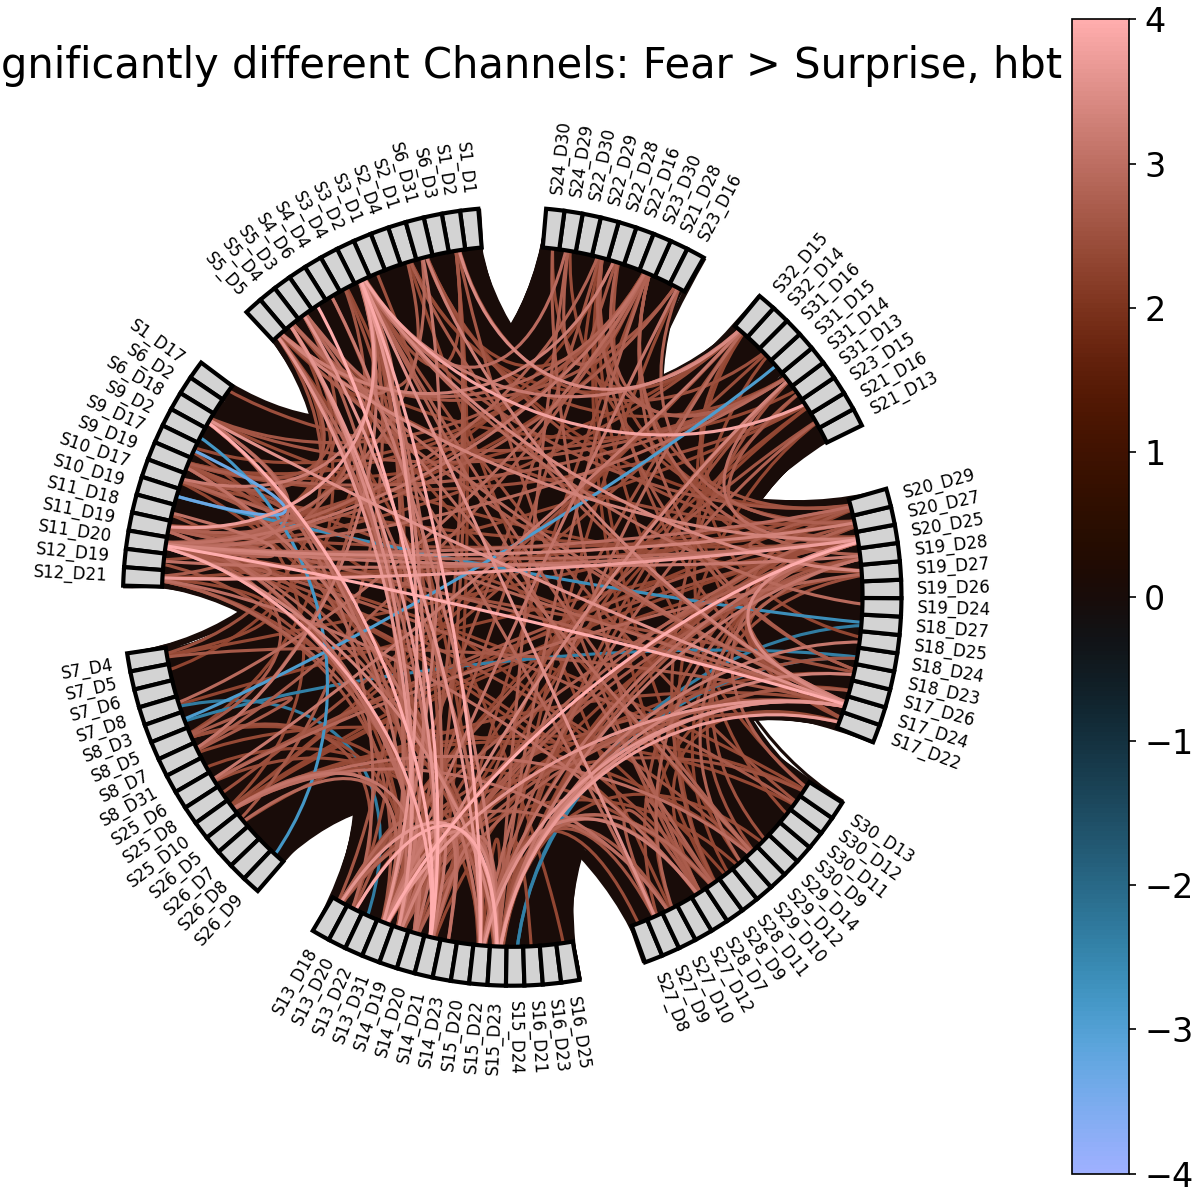
\includegraphics[width=0.32\textwidth]{C:/Users/super/OneDrive - Ontario Tech University/fNIRS_Emotions/plots/spectral_connectivity_time/chord_plots/group_level_t_tests_roi/emotion_Fear_Surprise.png}
  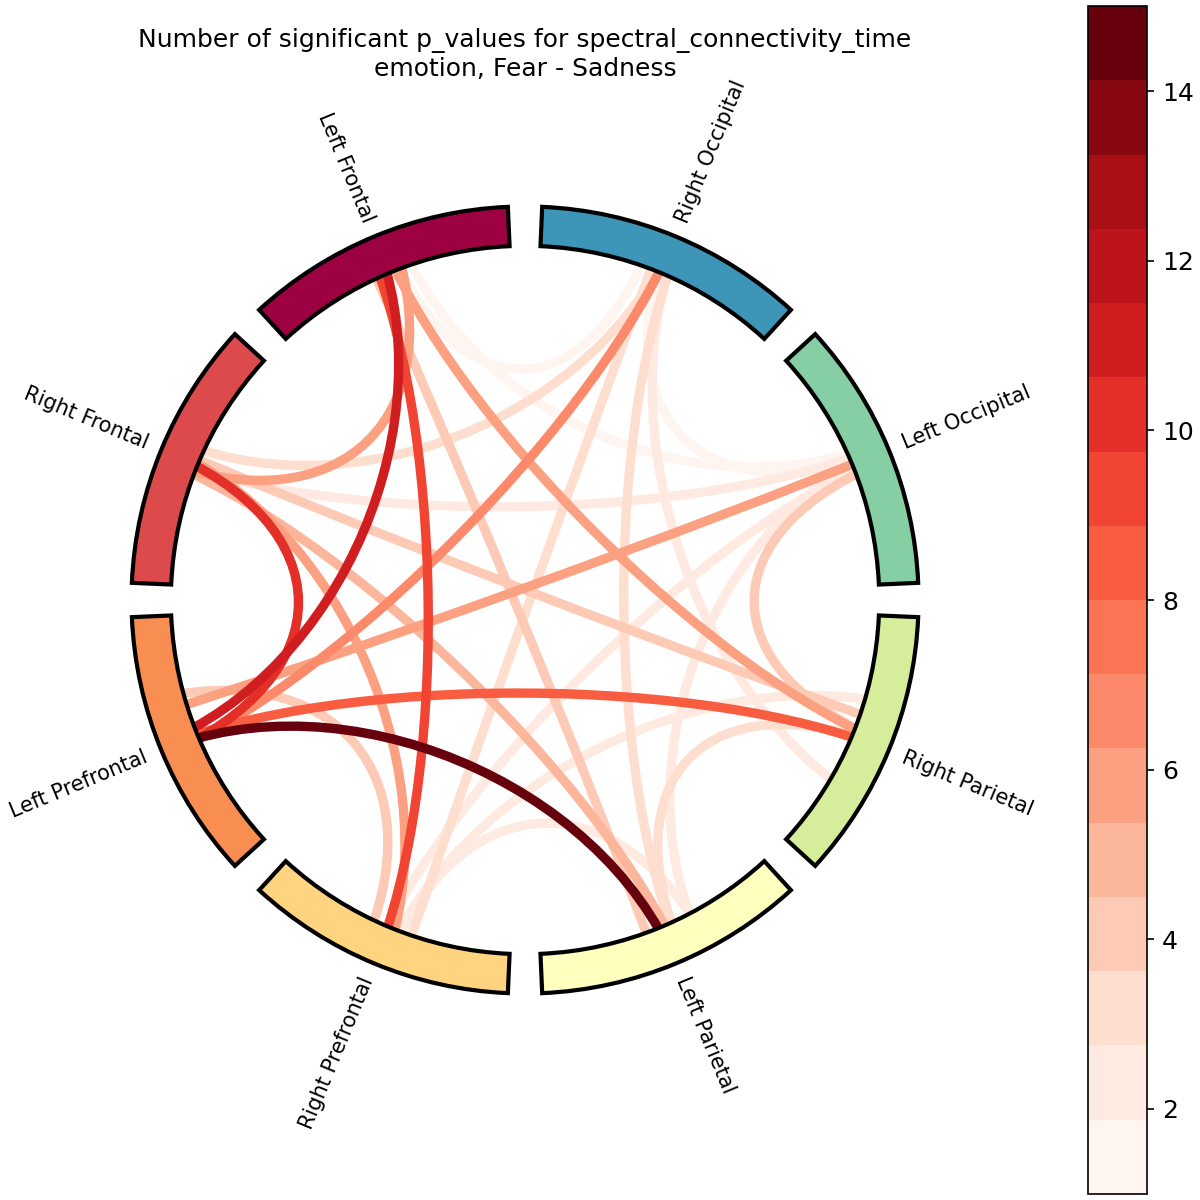
\includegraphics[width=0.32\textwidth]{C:/Users/super/OneDrive - Ontario Tech University/fNIRS_Emotions/plots/spectral_connectivity_time/chord_plots/group_level_t_tests_roi/emotion_Fear_Sadness.png}
  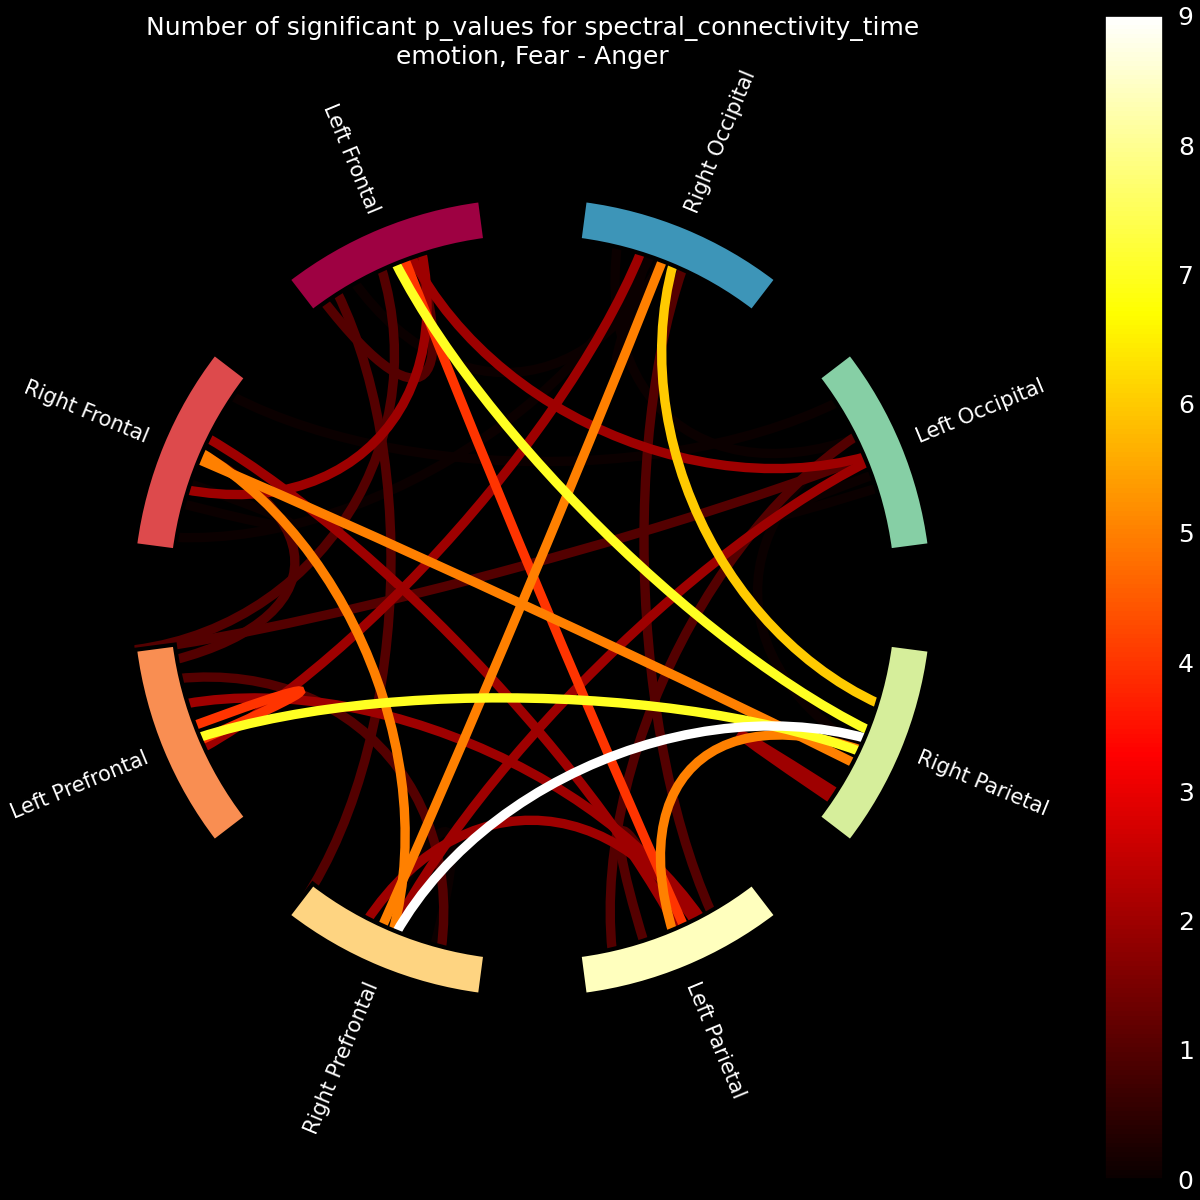
\includegraphics[width=0.32\textwidth]{C:/Users/super/OneDrive - Ontario Tech University/fNIRS_Emotions/plots/spectral_connectivity_time/chord_plots/group_level_t_tests_roi/emotion_Fear_Anger.png}
  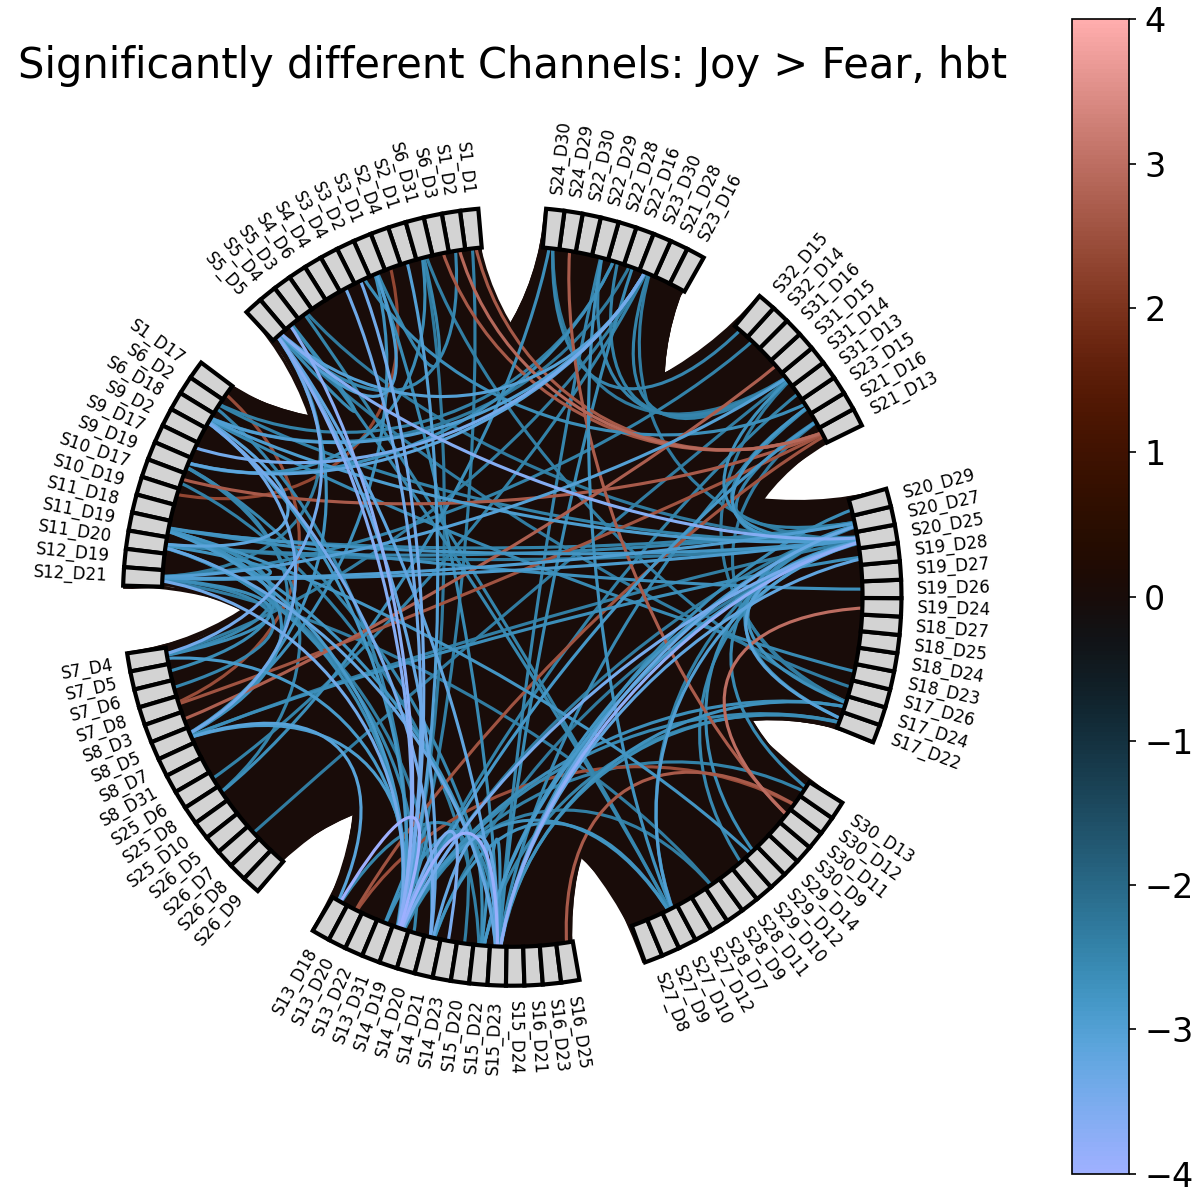
\includegraphics[width=0.32\textwidth]{C:/Users/super/OneDrive - Ontario Tech University/fNIRS_Emotions/plots/spectral_connectivity_time/chord_plots/group_level_t_tests_roi/emotion_Joy_Fear.png}
  \caption[FC: Emotion Contrasts (Fear)]{Functional connectivity results for Fear relative to the other emotions.}
  \label{fig:fc_emotion_analysis}
\end{figure}

A higher level summary of the functional connectivity results for all emotions is shown in Figure \ref{fig:fc_emotion_summary_analysis}, which shows the ratio of significant channels where the $t$-value was positive (red) or negative (blue) for each emotion pair.
We found a cluster of emotions (Anger, Fear, and Joy) that had much stronger connectivity compared to the other emotions, with Anger and Fear having slightly higher connectivity than Joy.
The other emotions (Neutral, Sadness, Surprise) had lower connectivity compared to Anger, Fear, and Joy, with Disgust having higher connectivity than Neutral. 
This lines up with Figure \ref{fig:fc_emotion_analysis}, which shows that processing Anger and Fear have higher connectivity relative to the other emotions. 

\begin{figure}[H]
  \centering
  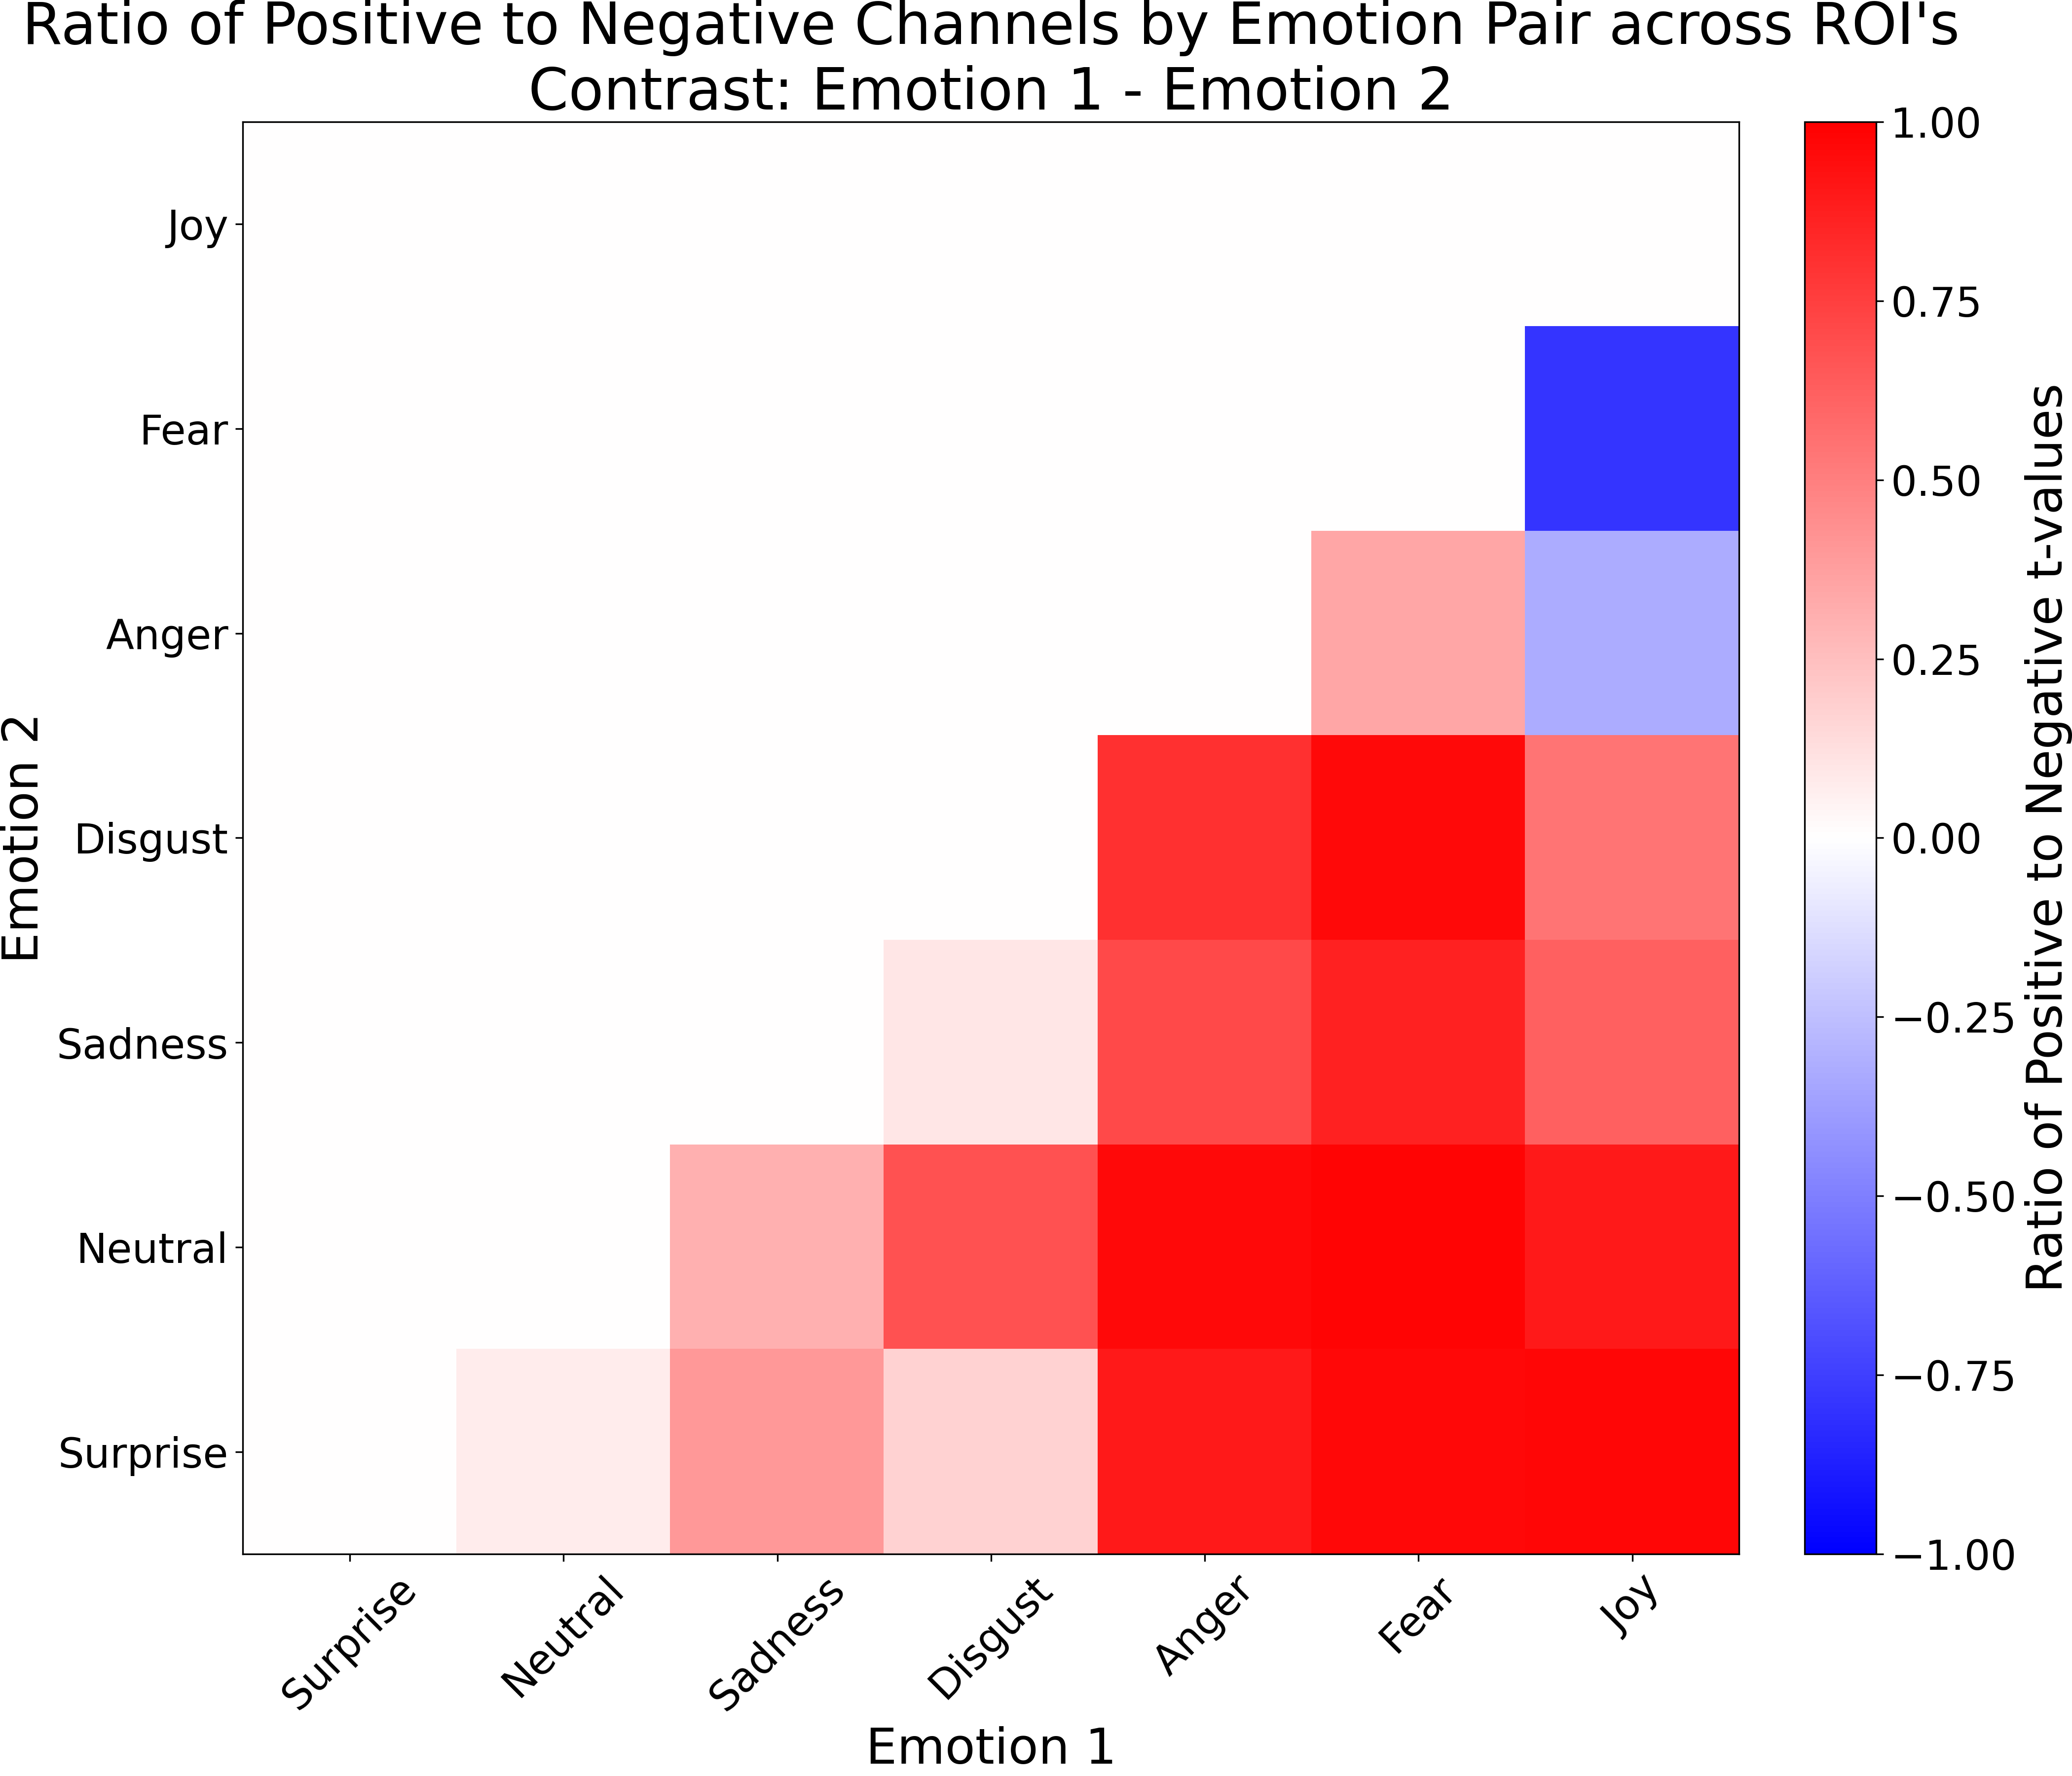
\includegraphics[width=0.87\textwidth]{C:/Users/super/OneDrive - Ontario Tech University/fNIRS_Emotions/plots/spectral_connectivity_time/emotion_analysis/emotion_contrast_heatmap.png}
  \caption[FC: Summary of Contrasts by Emotion Pair]{A heatmap summary of the functional connectivity results for the contrasts between different emotions across ROI's. 
  Red signifies that emotion 1 had a higher ratio of significant channels where the $t$-value was positive, while blue signifies that emotion 2 had a higher ratio of significant channels where the $t$-value was negative.
  The ratio was calculated by taking the difference of the count of significant channels where the $t$-value was positive and the count of significant channels where the $t$-value was negative, and dividing it by the total number of significant channels for that emotion pair.}
  \label{fig:fc_emotion_summary_analysis}
\end{figure}

To quantify the degree to which ROI's differed across emotion, significant channels across the brain were summed and plotted as a heatmap (Figure \ref{fig:fc_region_summary_analysis}).
Two regions, left occipital and right occipital, (marked with an asterisk), produced the least number of significant connections, suggesting that the connectivity within and between these regions are very similar in response to all emotions and that neural indices that differentiate emotion processing likely occur in brain regions outside of visual cortex.  
Three regions, left central/temporal, left parietal, and right central/temporal (marked with a caret), produced the most number of significant connections, suggesting that these regions are more variable in their connectivity patterns across emotions.

\begin{figure}[H]
  \centering
  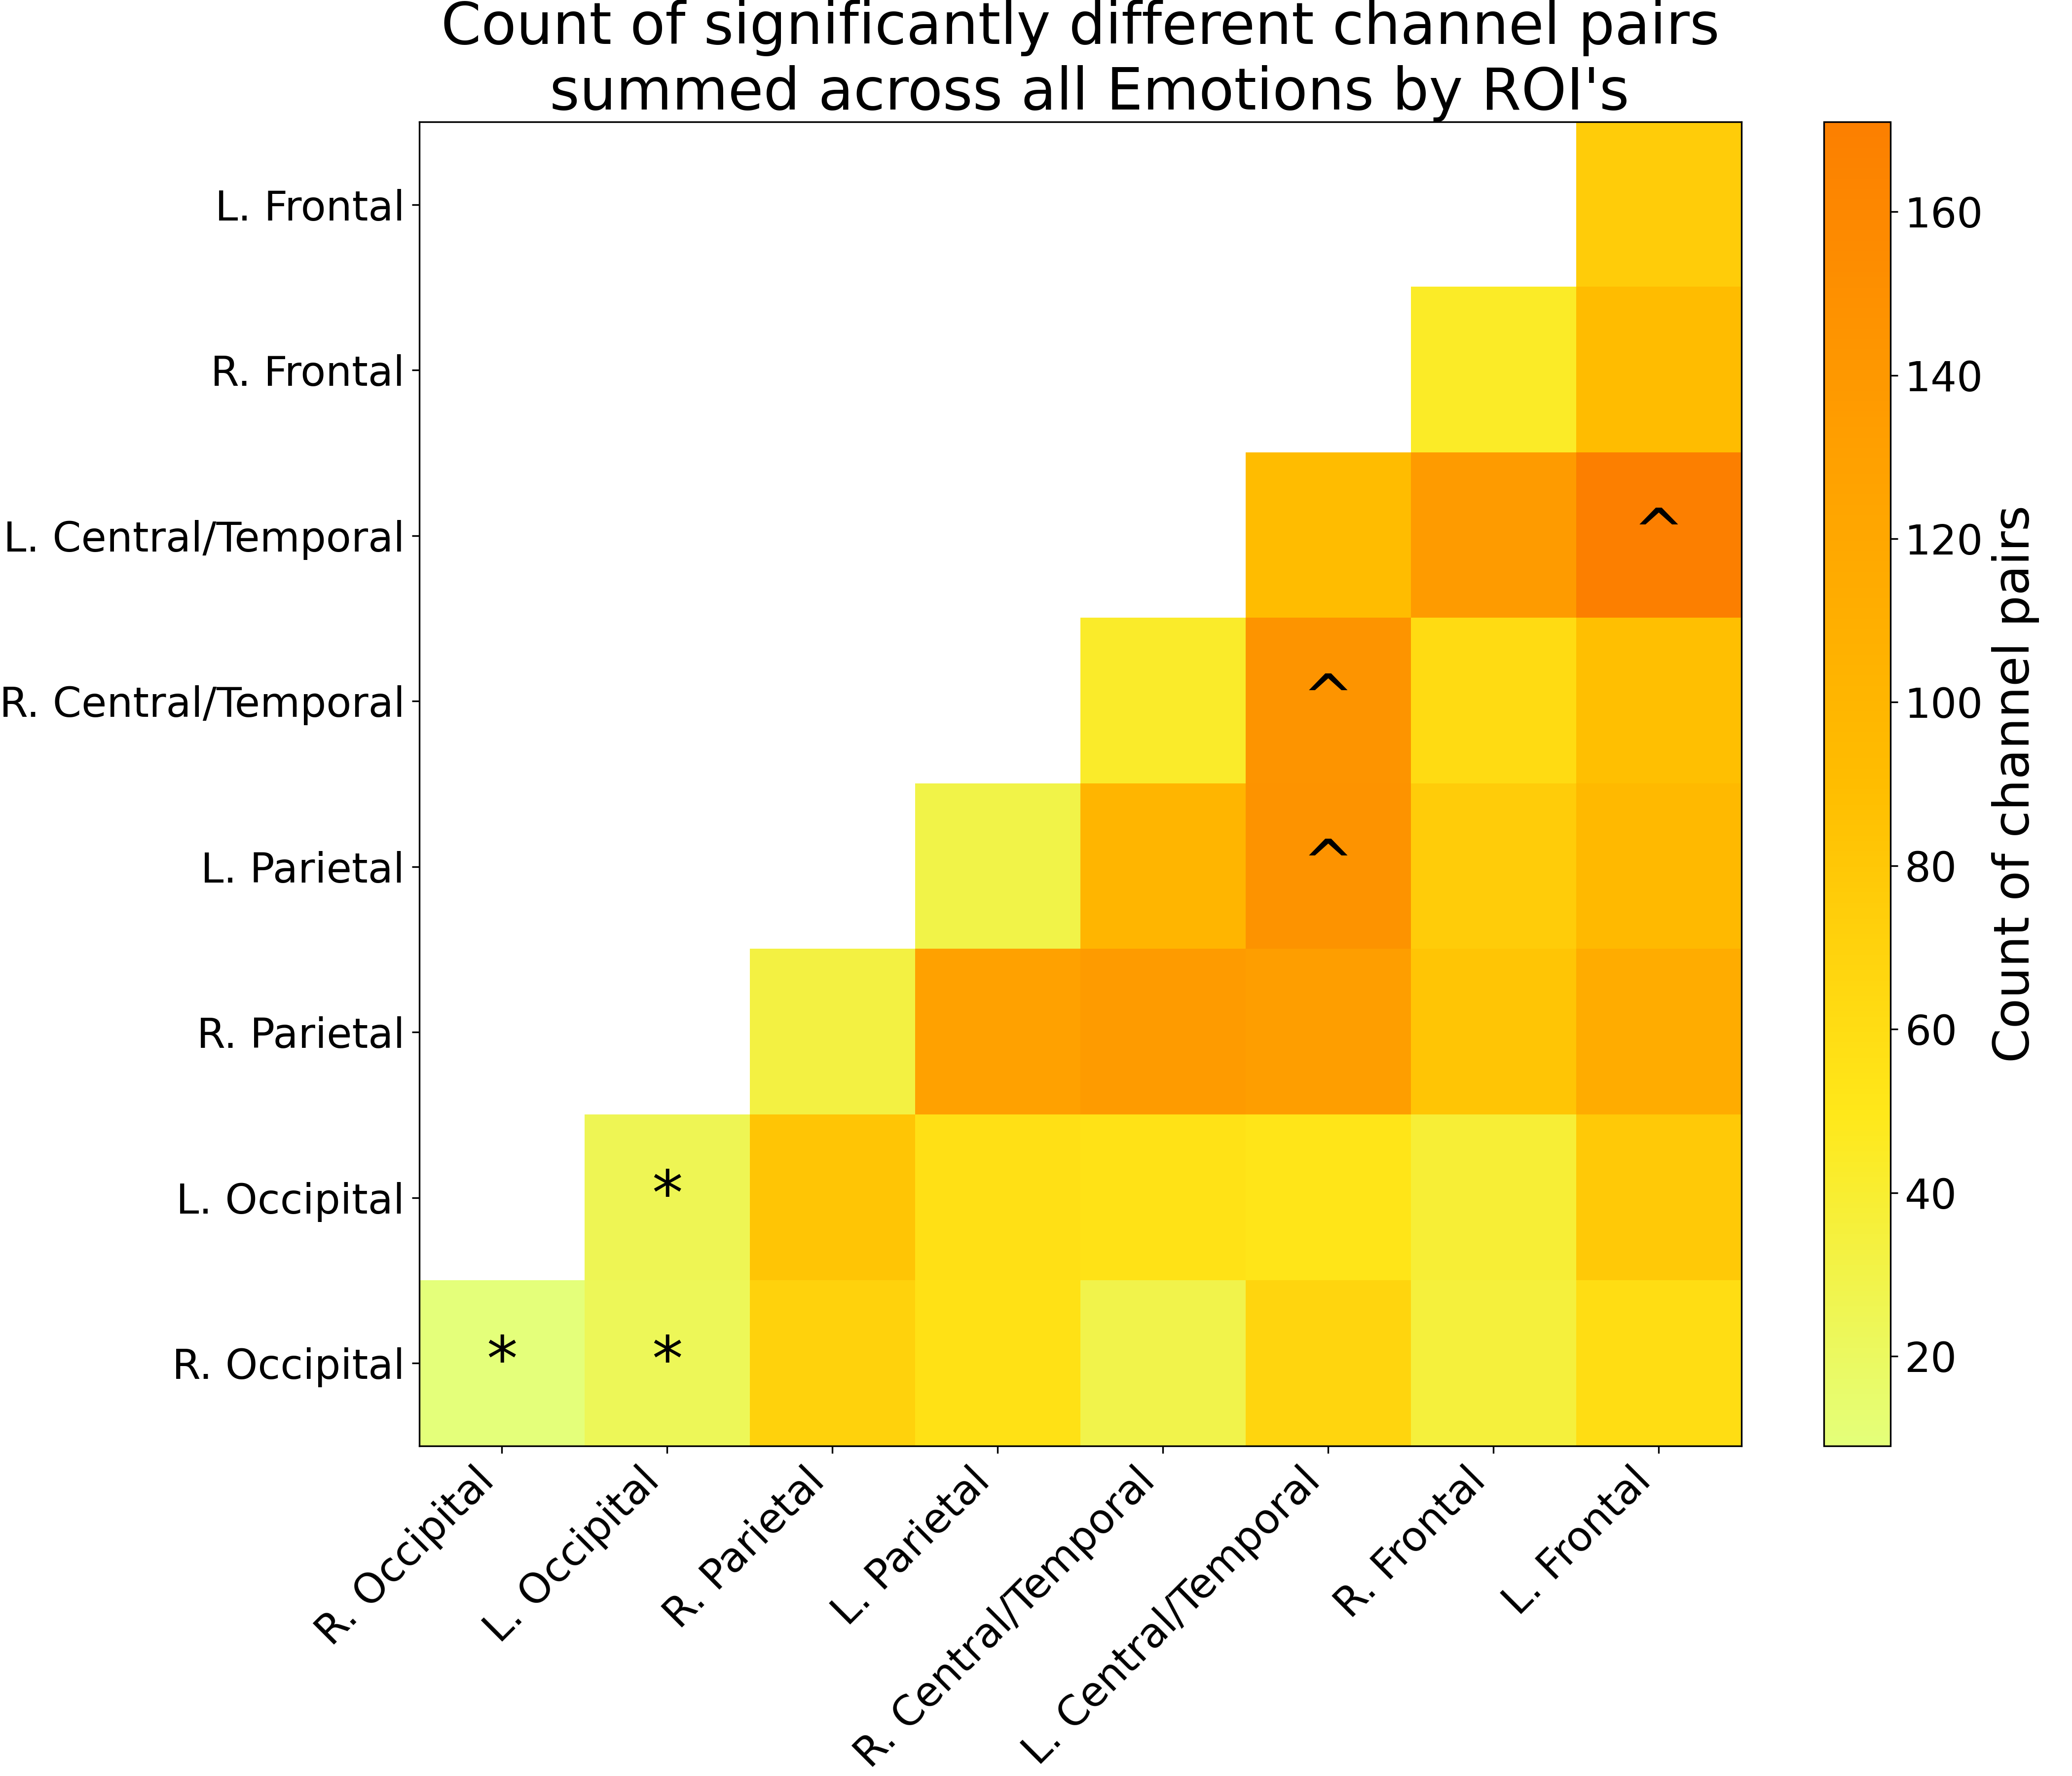
\includegraphics[width=0.87\textwidth]{C:/Users/super/OneDrive - Ontario Tech University/fNIRS_Emotions/plots/spectral_connectivity_time/emotion_analysis/region_contrast_heatmap.png}
  \caption[FC: Count of Significantly Different Channel Pairs by ROI]{A heatmap summary of the number of significantly different channel pairs for each ROI summed across all emotions. 
  The color bar on the right shows the number of significant channel pairs for each ROI, with brighter colors indicating a smaller number of significant channel pairs, and darker colors indicating a larger number of significant channel pairs.
  An asterisk (*) was placed on the 3 ROI's with the least number of significantly different channel pairs to indicate that these ROI's are more synchronized with each other than any other pair of ROI's, regardless of the emotion.
  A caret (\textasciicircum) was placed on the 3 ROI's with the most number of significantly different channel pairs to indicate that these ROI's are less synchronized with each other than any other pair of ROI's, regardless of the emotion.
  Note that ROI's can have differences within them, as each ROI is made up of multiple channels, and the differences are calculated between channels within the same ROI.}
  \label{fig:fc_region_summary_analysis}
\end{figure}

\noindent
\textbf{Differential Functional connectivity profiles in response to emotion across face type}

The interaction of face type with emotion, Real $>$ Virtual within each emotion (Figure \ref{fig:fc_real_vs_virtual_emotion_analysis}) revealed significant differences in functional connectivity across the brain.
We found that processing Anger on virtual faces elicited greater connectivity between the left frontal to right central/temporal, left frontal to right frontal, and within the left frontal region, compared to processing Anger on real faces.
Processing Disgust on virtual faces elicited greater connectivity between the left frontal to left parietal, right frontal to left parietal, right frontal to left central/temporal, left frontal to left occipital, and right central/temporal to right parietal, compared to processing Disgust on real faces.
Processing Fear on virtual faces elicited greater connectivity between many ROI's, particularly the left frontal to left occipital regions, between the left/right occipital regions, and between the left/right central/temporal and left/right occipital regions, compared to processing Fear on real faces.
Processing Neutral on virtual faces elicited greater connectivity between the left frontal to right frontal, left/right frontal to right parietal, and left/right parietal regions, compared to processing Neutral on real faces.
Processing Sadness on real faces elicited greater connectivity between the left frontal to right central/temporal, left central/temporal to right parietal, left central/temporal to right occipital, and right central/temporal to left parietal regions, compared to processing Sadness on virtual faces.
Processing Surprise on real faces elicited greater connectivity between many ROI's, such as the left frontal to left/right central/temporal, left frontal to right parietal, left/right central/temporal to left/right parietal, and within the left/right central/temporal regions, compared to processing Surprise on virtual faces.
Processing Joy on real faces elicited greater connectivity between the left/right central/temporal to right parietal, and within right parietal regions, whereas processing Joy on virtual faces elicited greater connectivity between the left central/temporal to left/right occipital regions. 
Overall, these results indicate that the effect of face type on functional connectivity varies by emotion, with virtual faces generally eliciting greater connectivity for negative emotions (Anger, Disgust, Fear, Neutral), while real faces tend to elicit greater connectivity for positive emotions (Sadness, Surprise, Joy), and the specific brain regions involved differ across emotions.
Like the GLM results, this indicates that the neural response to emotional expressions is modulated by the realism of the face stimuli. 
The full table of the functional connectivity contrasts for all main effects and interactions can be found in Appendix \ref{tab:appendix_fc_emotion_analysis}.

\begin{figure}[H]
  \centering
  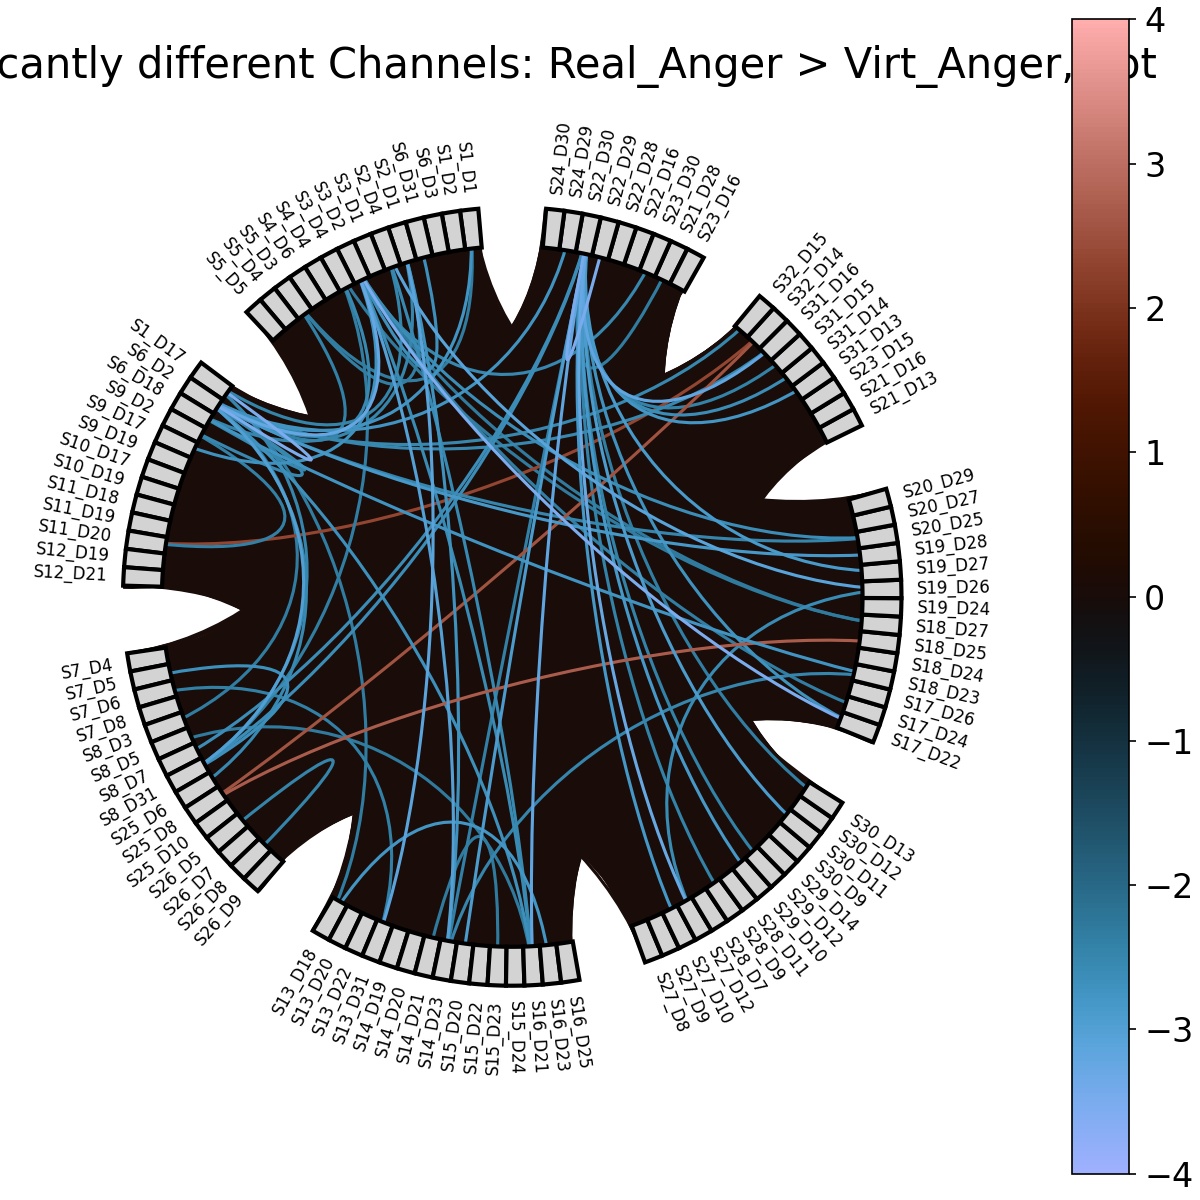
\includegraphics[width=0.32\textwidth]{C:/Users/super/OneDrive - Ontario Tech University/fNIRS_Emotions/plots/spectral_connectivity_time/chord_plots/group_level_t_tests_roi/face_type_emotion_Real_Anger_Virt_Anger.png}
  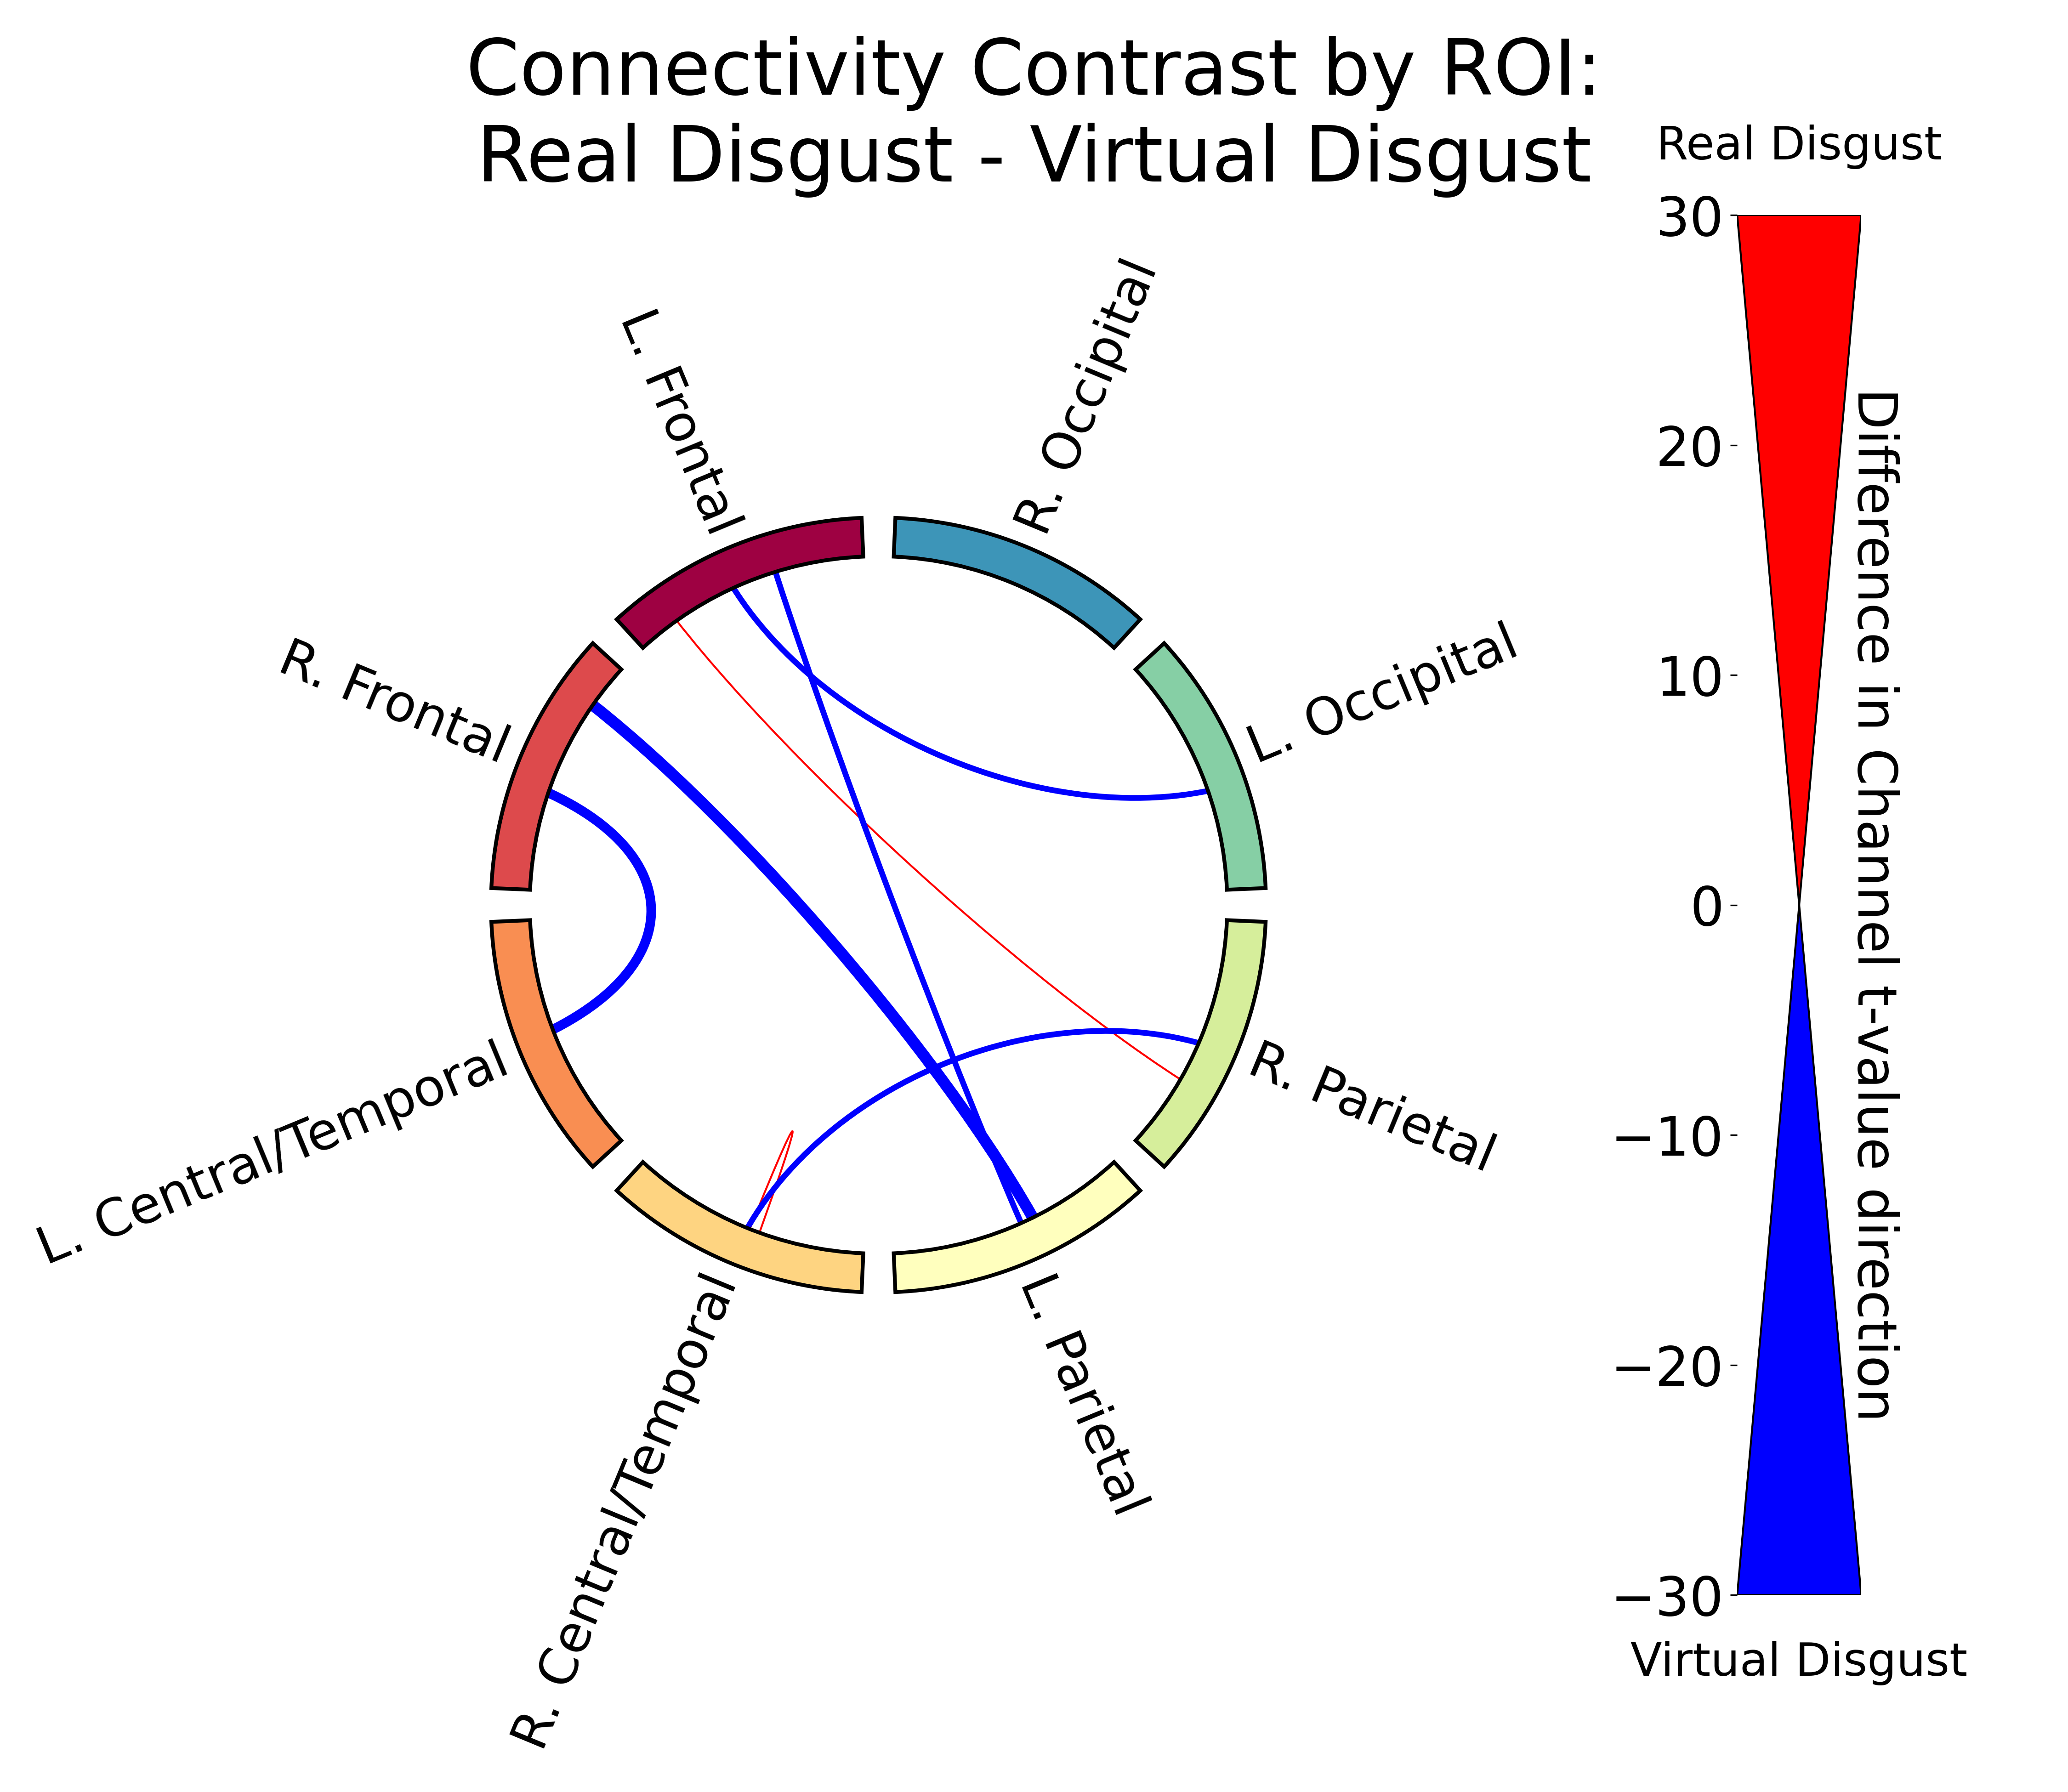
\includegraphics[width=0.32\textwidth]{C:/Users/super/OneDrive - Ontario Tech University/fNIRS_Emotions/plots/spectral_connectivity_time/chord_plots/group_level_t_tests_roi/face_type_emotion_Real_Disgust_Virt_Disgust.png}
  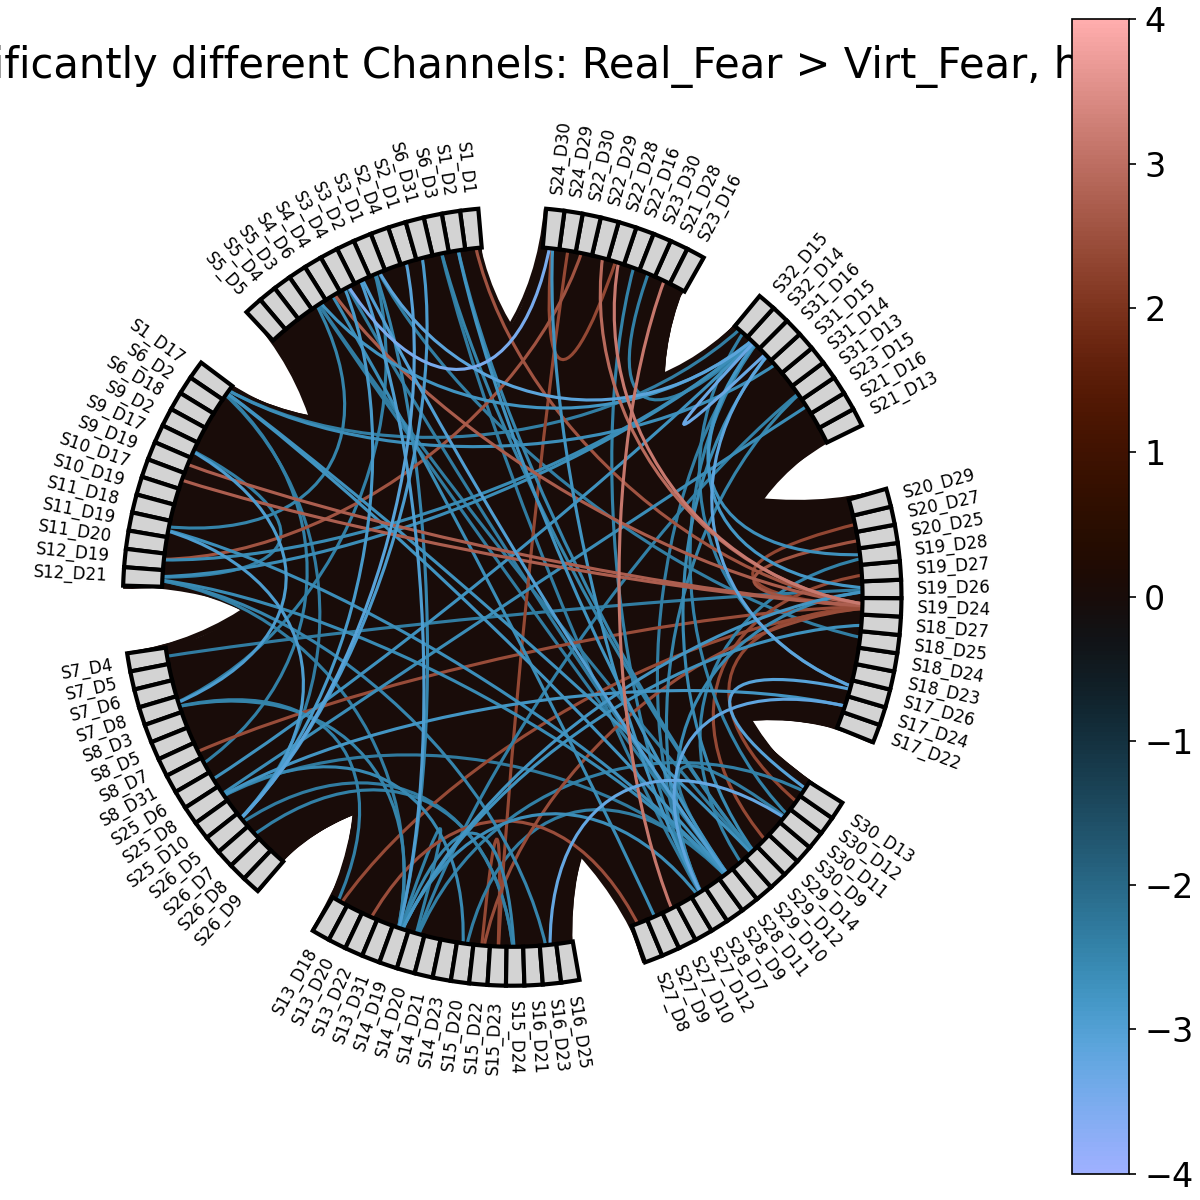
\includegraphics[width=0.32\textwidth]{C:/Users/super/OneDrive - Ontario Tech University/fNIRS_Emotions/plots/spectral_connectivity_time/chord_plots/group_level_t_tests_roi/face_type_emotion_Real_Fear_Virt_Fear.png}
  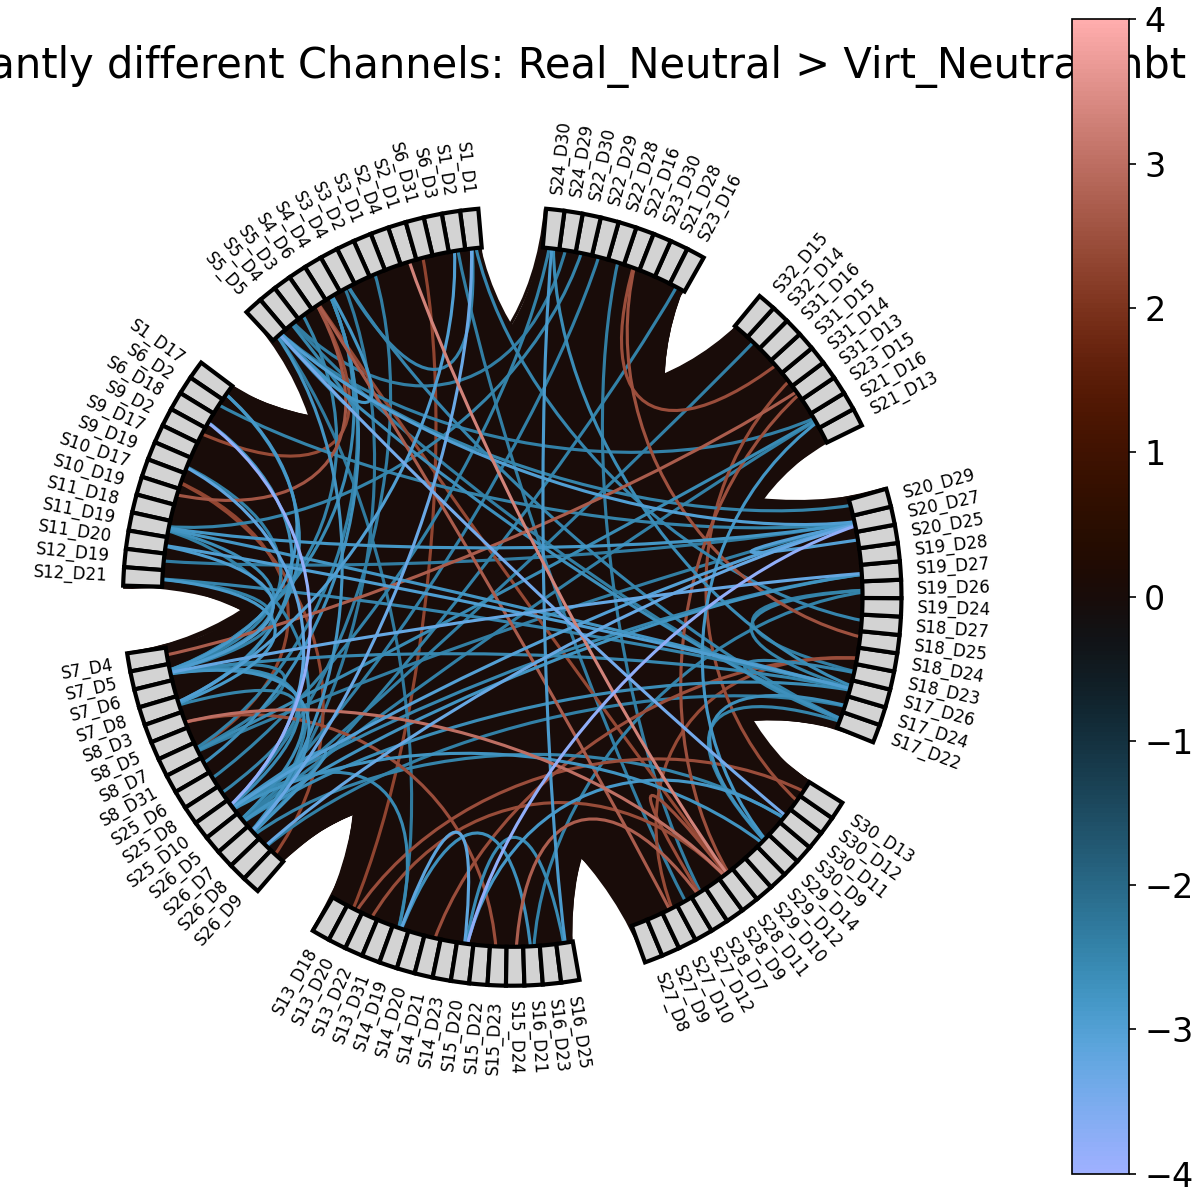
\includegraphics[width=0.32\textwidth]{C:/Users/super/OneDrive - Ontario Tech University/fNIRS_Emotions/plots/spectral_connectivity_time/chord_plots/group_level_t_tests_roi/face_type_emotion_Real_Neutral_Virt_Neutral.png}
  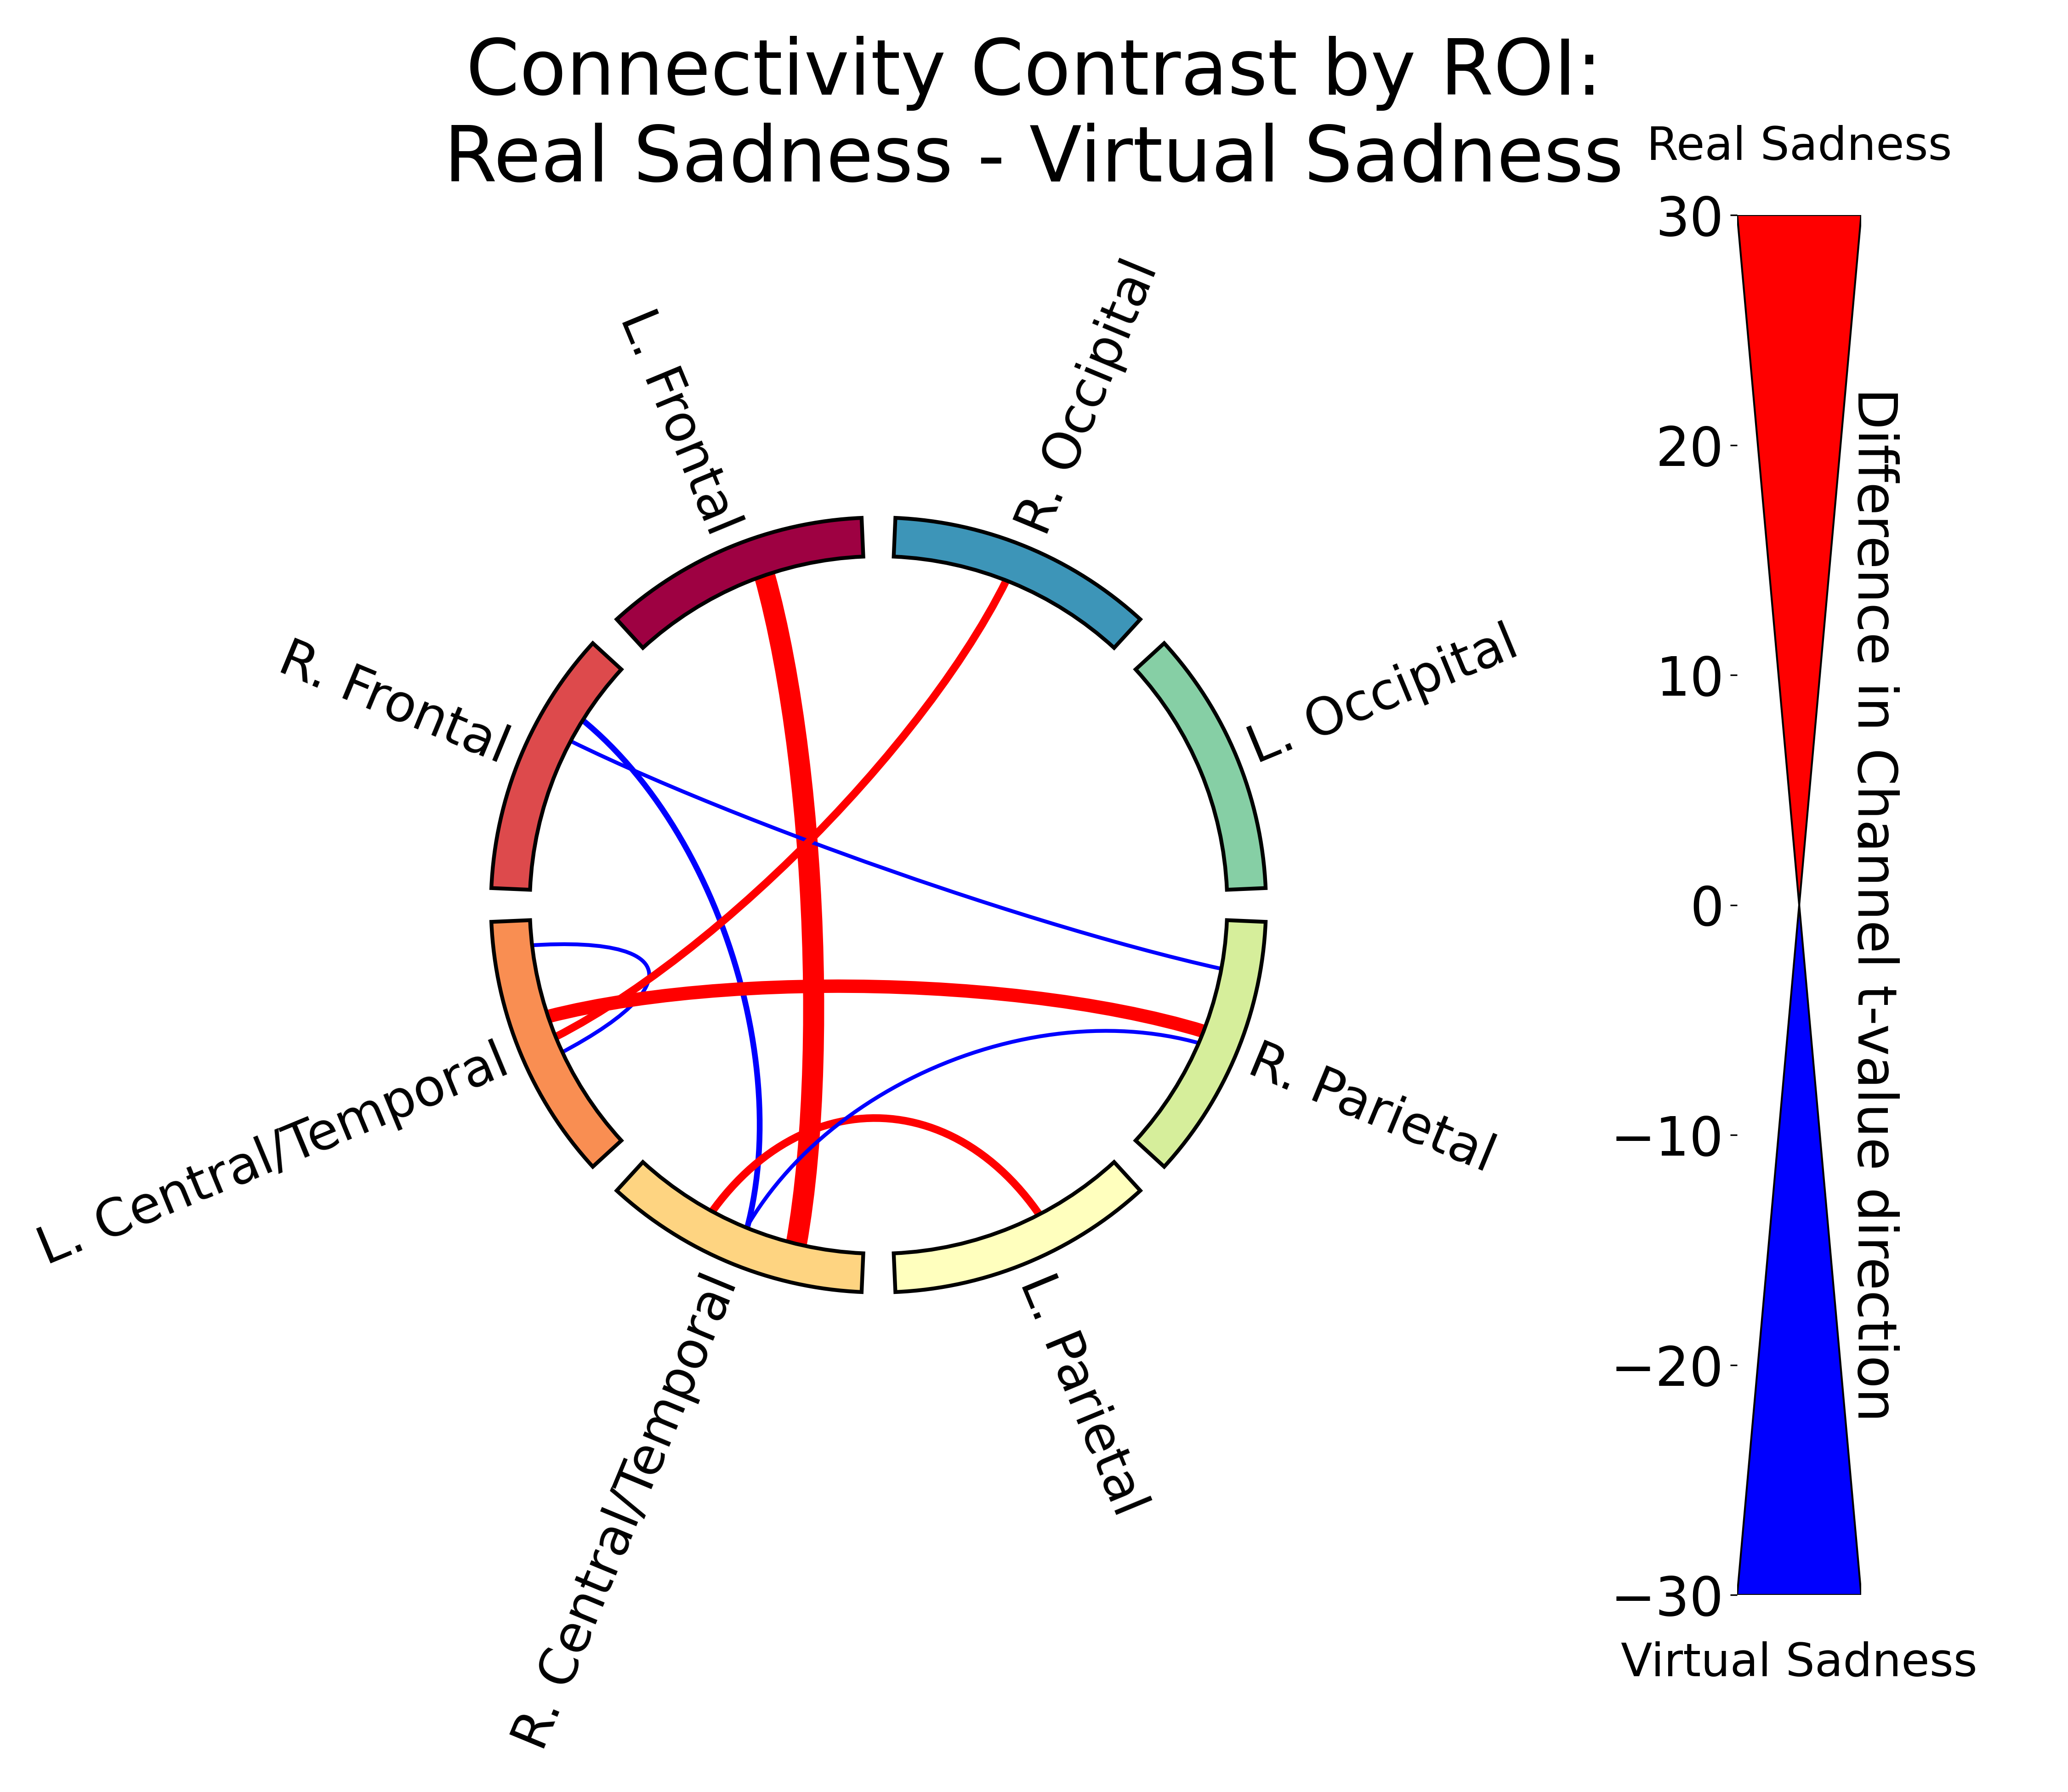
\includegraphics[width=0.32\textwidth]{C:/Users/super/OneDrive - Ontario Tech University/fNIRS_Emotions/plots/spectral_connectivity_time/chord_plots/group_level_t_tests_roi/face_type_emotion_Real_Sadness_Virt_Sadness.png}
  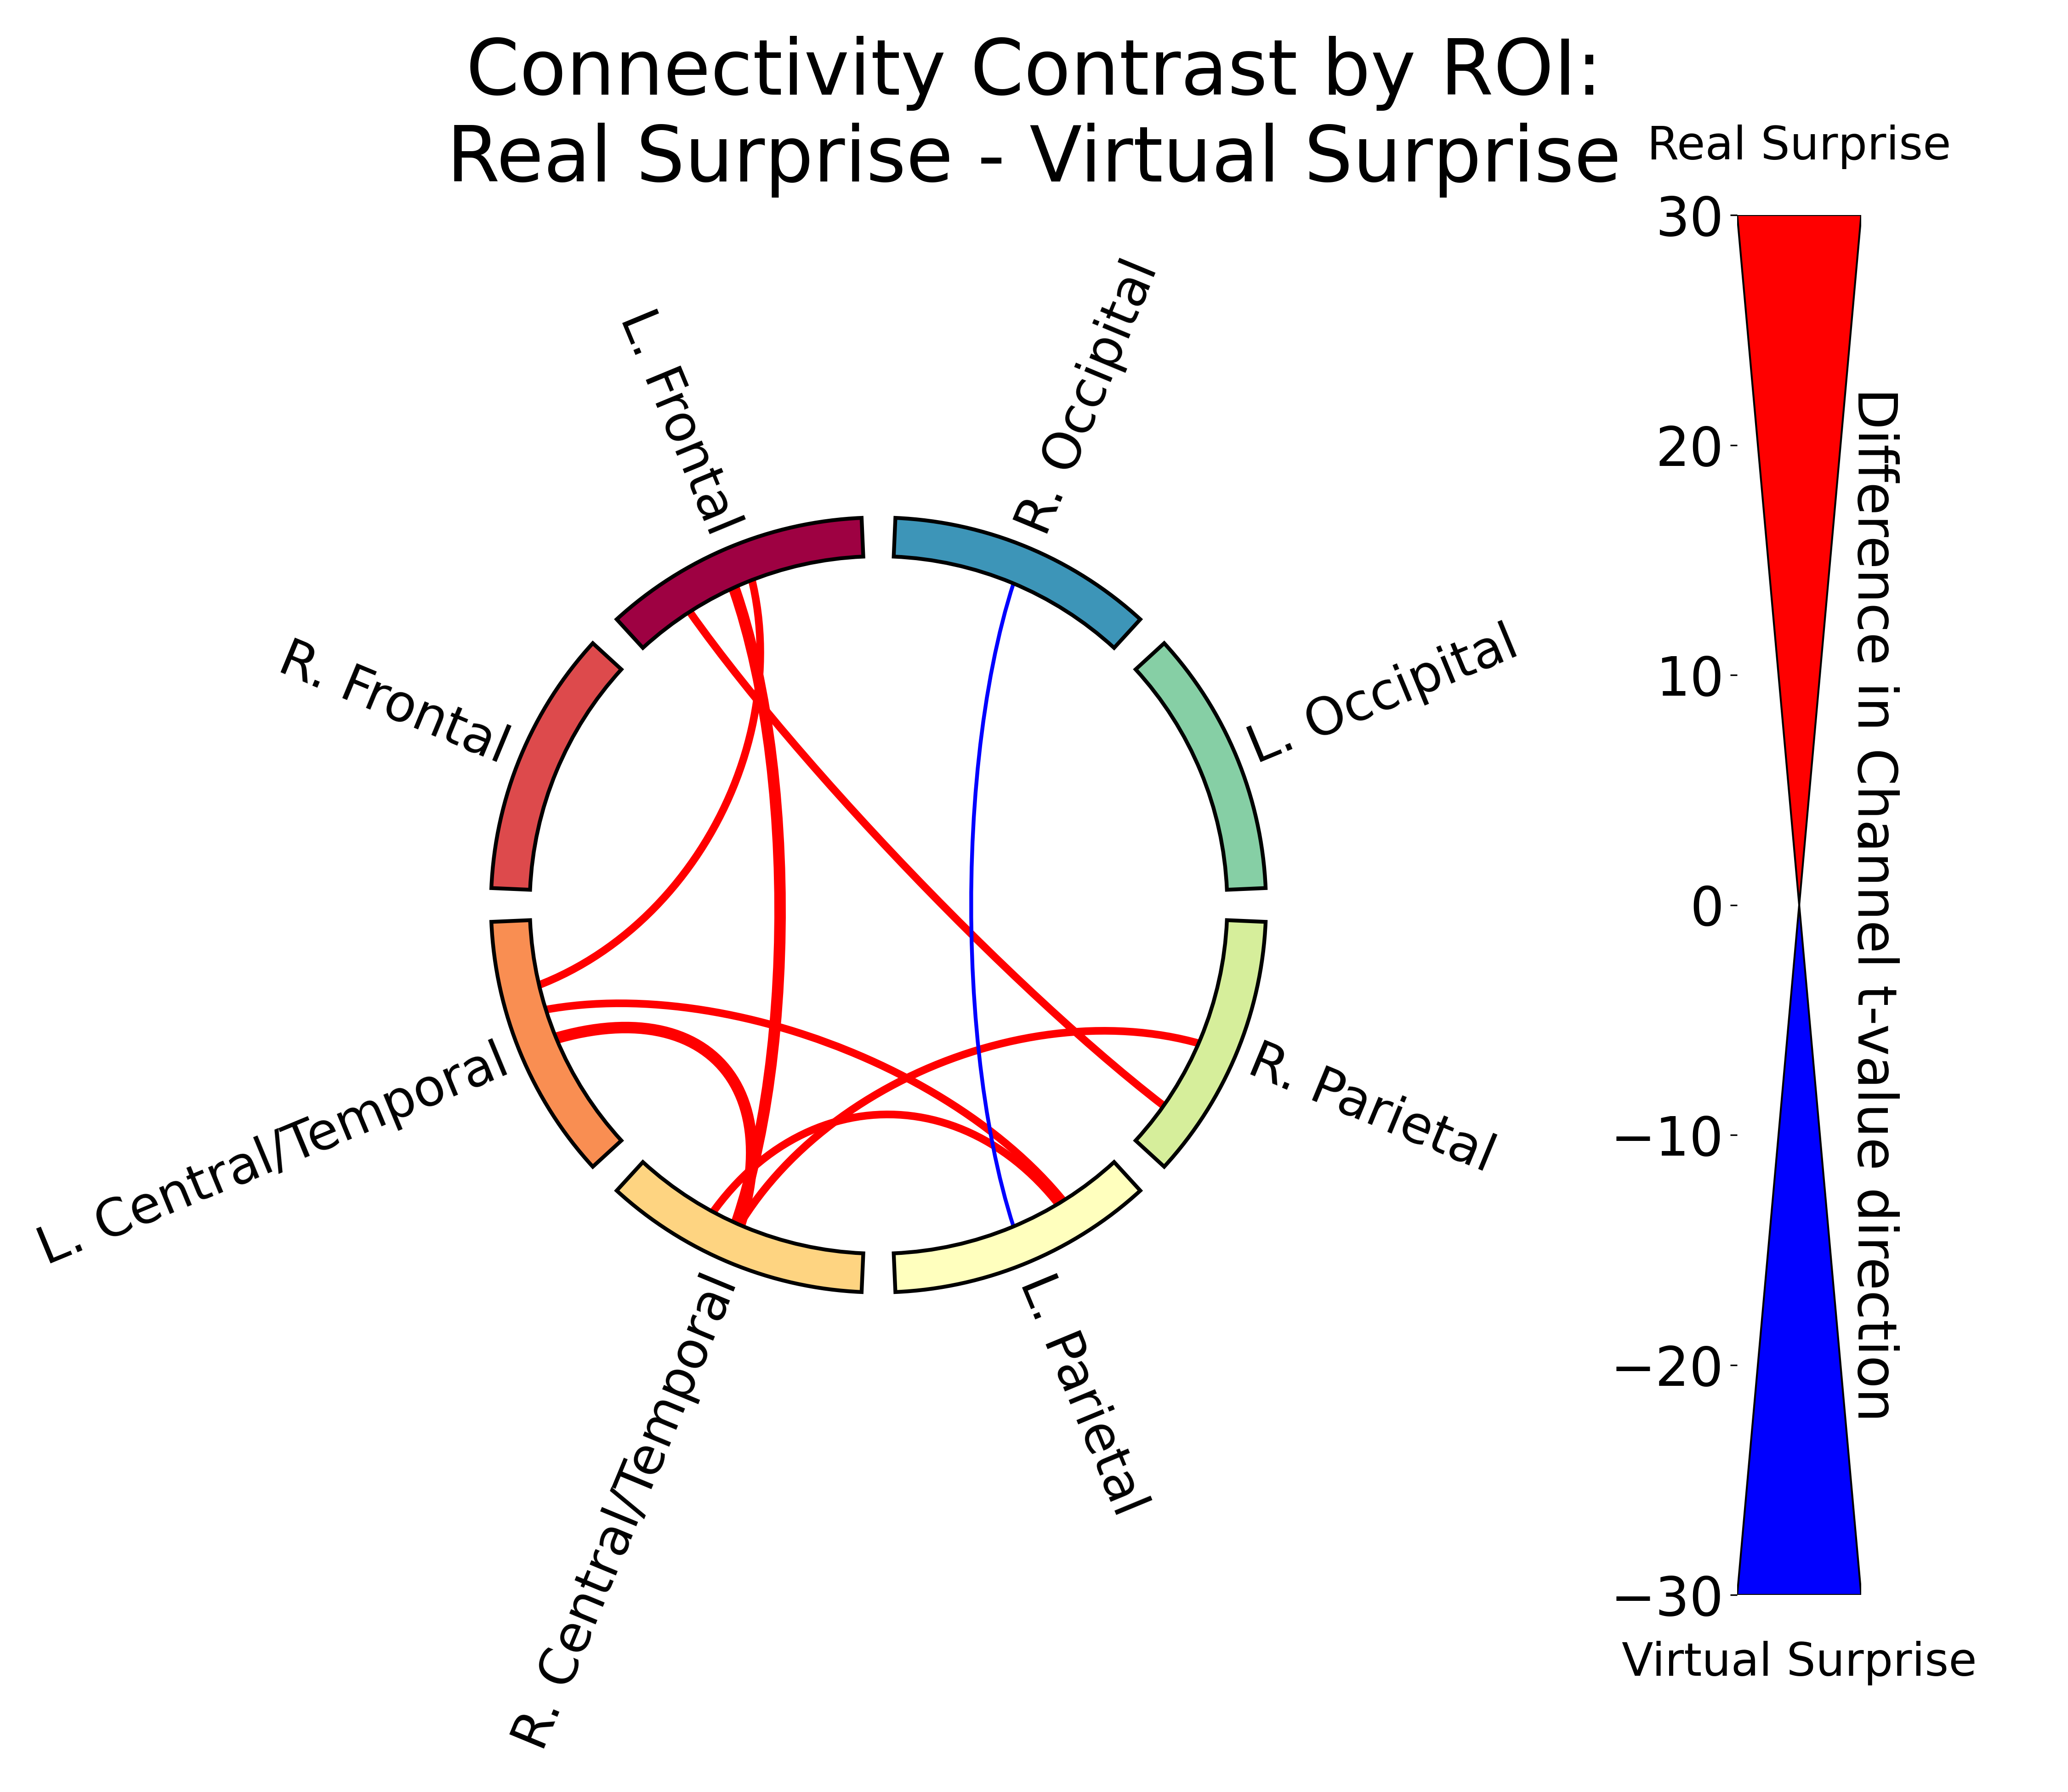
\includegraphics[width=0.32\textwidth]{C:/Users/super/OneDrive - Ontario Tech University/fNIRS_Emotions/plots/spectral_connectivity_time/chord_plots/group_level_t_tests_roi/face_type_emotion_Real_Surprise_Virt_Surprise.png}
  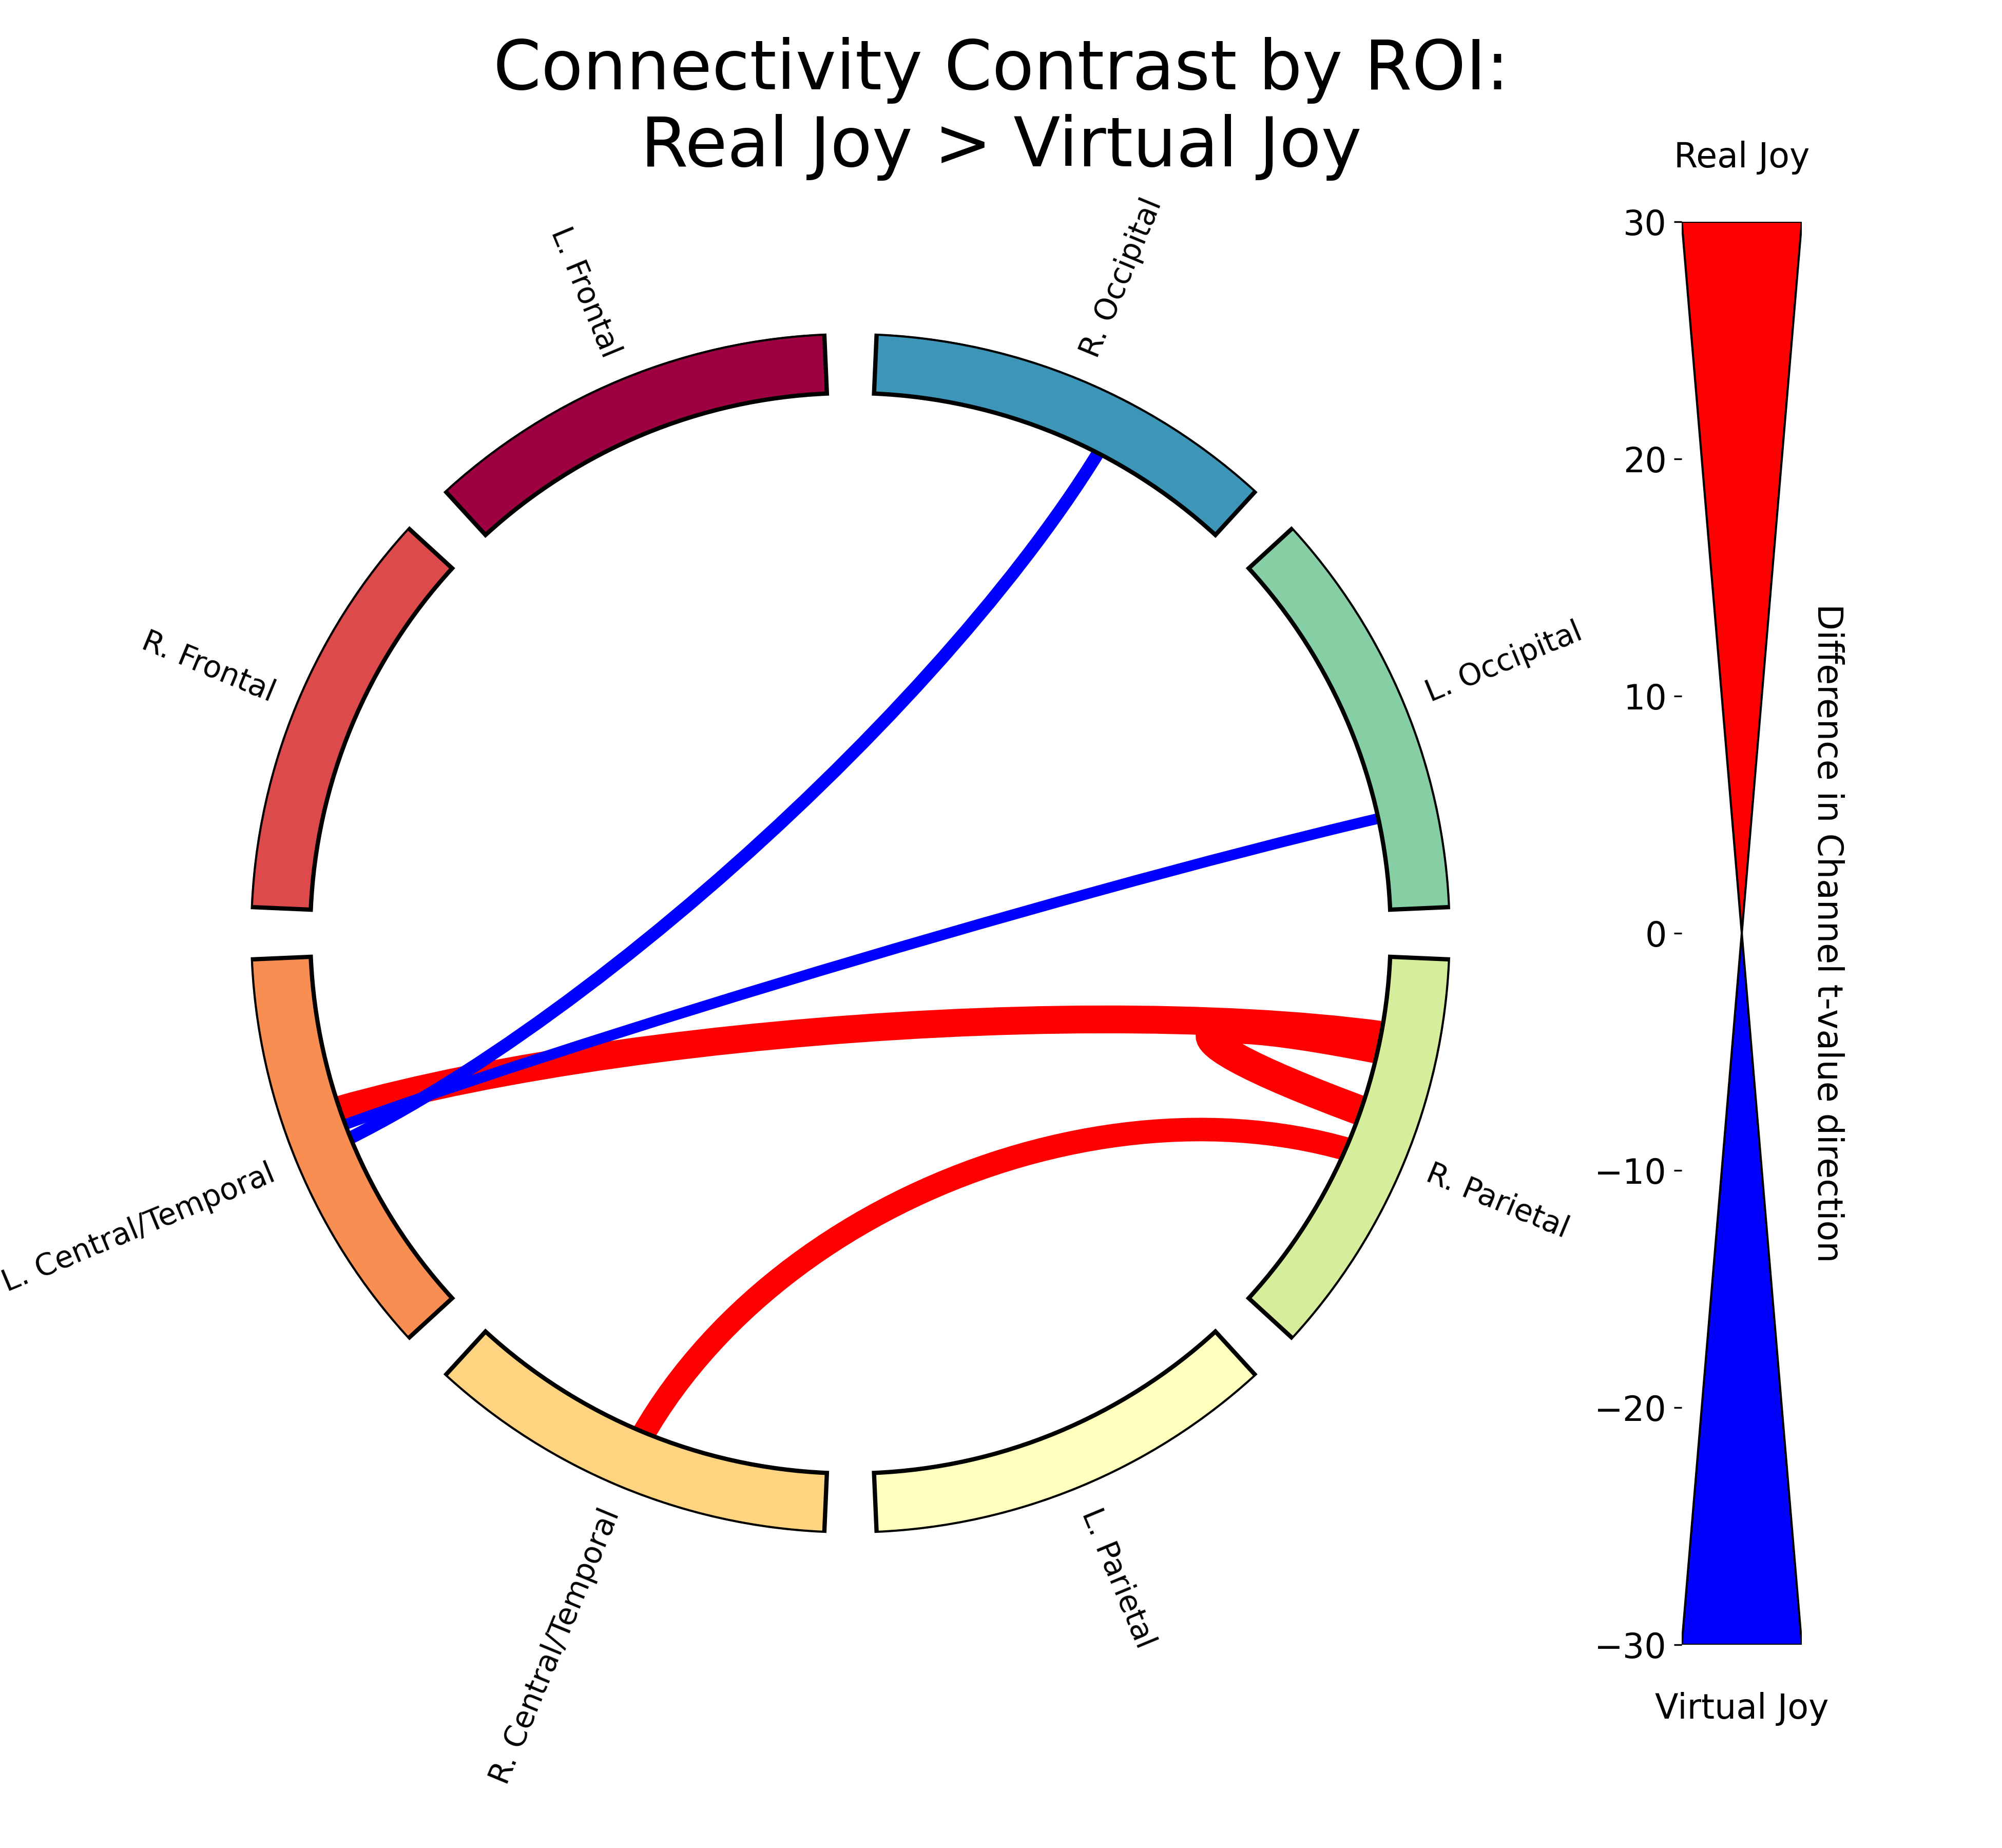
\includegraphics[width=0.32\textwidth]{C:/Users/super/OneDrive - Ontario Tech University/fNIRS_Emotions/plots/spectral_connectivity_time/chord_plots/group_level_t_tests_roi/face_type_emotion_Real_Joy_Virt_Joy.png}
  \caption[FC: Face Type \texorpdfstring{$\times$}{x} Emotion Contrasts]{Functional connectivity results for the contrast between real and virtual conditions within each emotion.}
  \label{fig:fc_real_vs_virtual_emotion_analysis}
\end{figure}

\section{Memory Task Results}
A two-way Type III ANOVA revealed a significant main effect of face type, $F(1,4802)=7.96$, $p=0.0048$, indicating that memory performance was higher for real faces compared to virtual faces, as shown in Figure \ref{fig:memory_task_results}.
There was no significant main effect of emotion, $F(6,4802)=0.83$, $p=0.55$, nor a significant interaction between face type and emotion, $F(6,4802)=0.46$, $p=0.84$. 
These findings suggest that while the realism of the face influences memory performance, the specific emotional expression does not have a significant impact on memory accuracy.
The full ANOVA table is shown in Appendix \ref{tab:appendix_memory_task_anova}.

\begin{figure}[H]
  \centering
  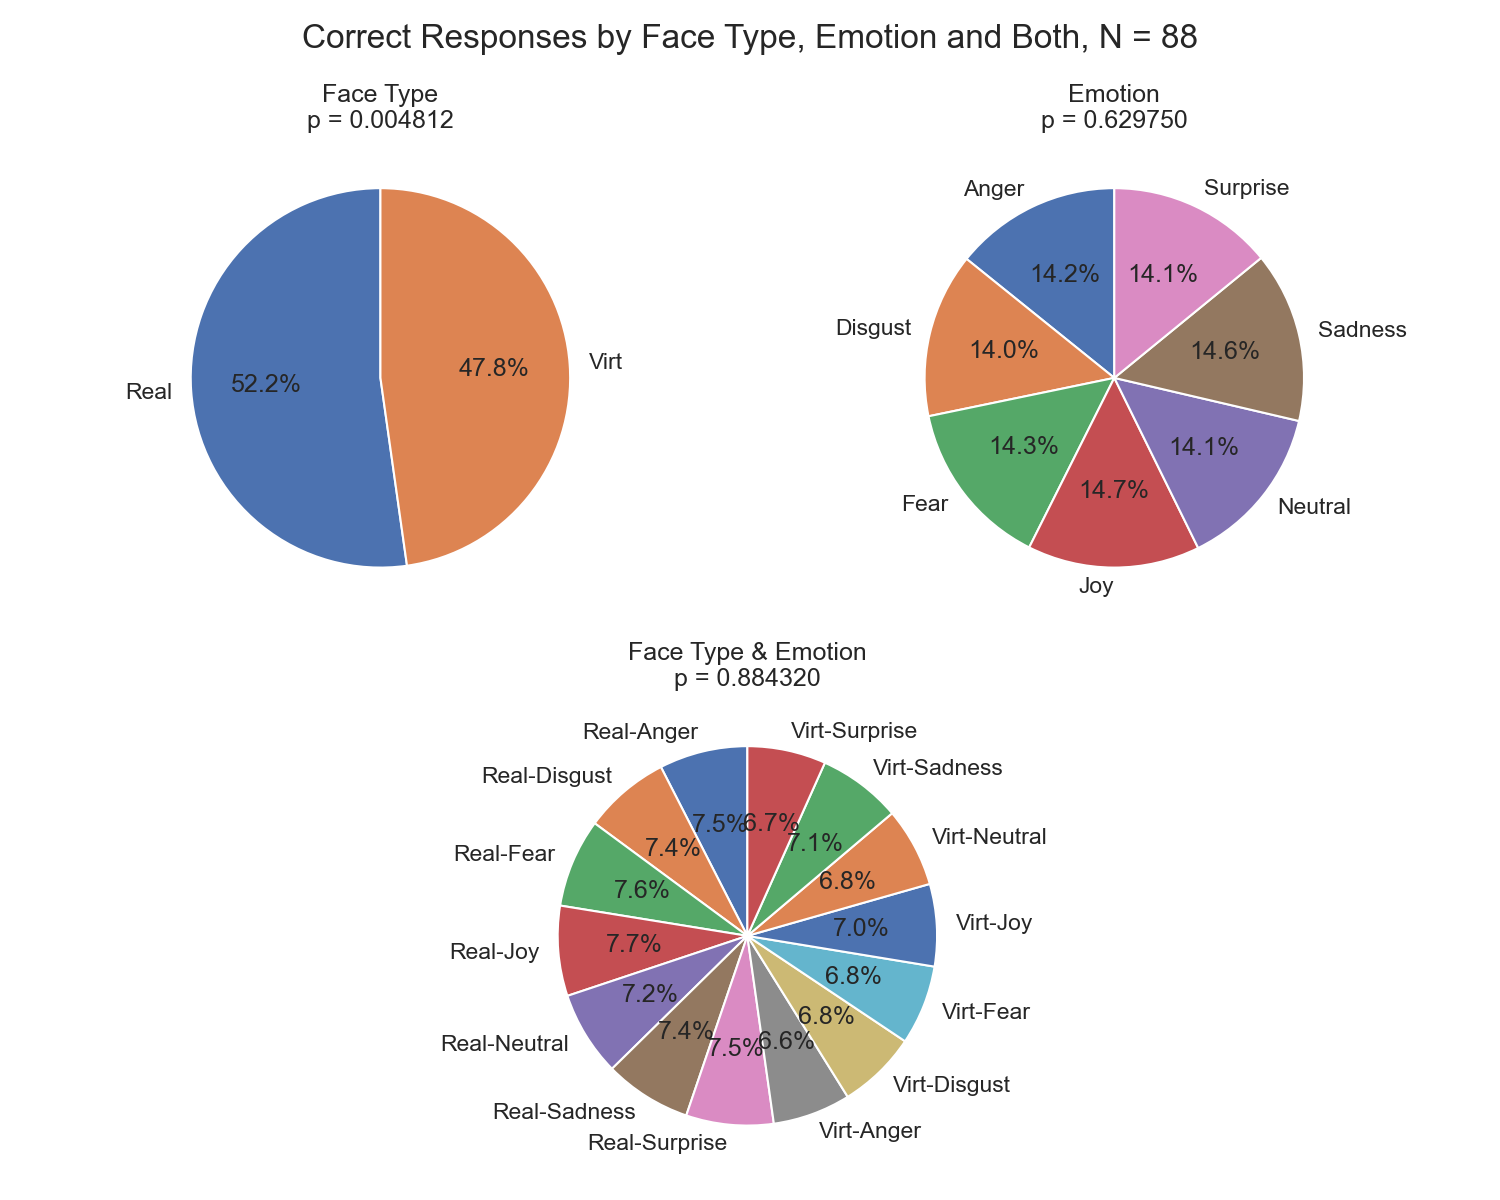
\includegraphics[width=1\textwidth]{C:/Users/super/OneDrive - Ontario Tech University/fNIRS_Emotions/plots/behavioural_responses/correct_responses_by_face_type_emotion.png}
  \caption[Correct Memory Task Responses by Face Type and Emotion]{Proportion correct by condition in the memory task, plotted separately for real and virtual faces, for each emotion, and the interaction between face type and emotion. 
  The $p$-values indicate the significance of the main effects and interaction. }
  \label{fig:memory_task_results}
\end{figure}